\documentclass[%
11pt,%
%oneside,%
twoside,%
%twocolumn,%
titlepage,%
%fleqn,%
%a4page,%
german,%
headsepline%
]{scrartcl}

\usepackage{lastpage}
\usepackage{geometry}
\usepackage{graphicx}
\usepackage[utf8]{inputenc}
\usepackage[ngerman]{babel}
\usepackage{lscape}
\usepackage[framemethod=TikZ]{mdframed}
\usepackage[most]{tcolorbox}
\usepackage{mymath}
\usepackage{units}
\usepackage{nicefrac}
\usepackage{pgf,tikz}
\usepackage{pgfplots}
\pgfplotsset{width=10cm,compat=1.9}

\usetikzlibrary{arrows}
\usetikzlibrary{calc, shapes, backgrounds}
\usepackage{colortbl}
\usepackage{hhline}
\usepackage{multirow}
\usepackage[extendedchars]{grffile}
\usepackage{caption}
\usepackage{multicol,calc}
\usepackage{blindtext}
\usepackage{pdfpages}
\usepackage{hyperref}
\usepackage{wrapfig}
\usepackage{booktabs}

\usepackage{marginnote}
\usepackage{qrcode}
\qrset{height=9ex}

%Gothic-Font
\usepackage{oldgerm}
\usepackage{pifont}
\usepackage{yfonts}

% footnote-symbols
\usepackage[symbol]{footmisc}
\renewcommand{\thefootnote}{\fnsymbol{footnote}}

% Command, um Tabellen-Spalten anzupassen
\newcommand{\spaltenheight}{\rule{0mm}{3ex}}
\newcommand{\spaltenwidth}{\rule{3cm}{0mm}}
\newcommand{\spaltensep}{\\[1ex]}
\doublerulesepcolor{white}

\usepackage{fontawesome} % FontAwesome, falls du ein Augensymbol brauchst
\definecolor{lightgray}{rgb}{0.7, 0.7, 0.7}
\newcommand{\faEyeLightGray}{\textcolor{lightgray}{\faEye}} % Custom command for the gray eye icon


% Pagestyle/Layout
\setlength{\parindent}{0pt} \setlength{\parskip}{1em}

\pagestyle{headings} % gemachte Einstellungen anwenden

% Farbig umrahmte Umgebung Satz 
 \definecolor{myblizzardblue}{HTML}{87CEEB}

\newcounter{satzz}[section]\setcounter{satzz}{0}
\renewcommand{\thesatz}{\arabic{section}.\arabic{satzz}}

\newenvironment{csatz}[1][]{%
    \refstepcounter{satzz}
 
    \ifstrempty{#1}%
    % if condition (without title)
    {\mdfsetup{%
        frametitle={%
            \tikz[baseline=(current bounding box.east),outer sep=0pt]
            \node[anchor=east,rectangle,fill=myblizzardblue]
            {\strut Satz~\thesatz};}
        }%
    % else condition (with title)
    }{\mdfsetup{%
        frametitle={%
            \tikz[baseline=(current bounding box.east),outer sep=0pt]
            \node[anchor=east,rectangle,fill=myblizzardblue]
            {\strut Satz~\thesatz:~#1};}%
        }%
    }%
% for both conditions
    \mdfsetup{%
        innertopmargin=10pt,linecolor=myblizzardblue,%
        backgroundcolor=whitesmoke,%
        linewidth=2pt,topline=true,%
        frametitleaboveskip=\dimexpr-\ht\strutbox\relax%
    }
 
\begin{mdframed}[]\relax}{%
\end{mdframed}}

% Farbig umrahmte Umgebung Theorem
\definecolor{mygraphblue}{HTML}{84B7E1}
\definecolor{whitesmoke}{HTML}{F5F5F5}

\newcounter{theo}[section]\setcounter{theo}{0}
\renewcommand{\thetheo}{\arabic{section}.\arabic{theo}}

\newenvironment{ctheo}[1][]{%
    \refstepcounter{theo}
 
    \ifstrempty{#1}%
    % if condition (without title)
    {\mdfsetup{%
        frametitle={%
            \tikz[baseline=(current bounding box.east),outer sep=0pt]
            \node[anchor=east,rectangle,fill=mygraphblue]
            {\strut Theorem~\thetheo};}
        }%
    % else condition (with title)
    }{\mdfsetup{%
        frametitle={%
            \tikz[baseline=(current bounding box.east),outer sep=0pt]
            \node[anchor=east,rectangle,fill=mygraphblue]
            {\strut Theorem~\thetheo:~#1};}%
        }%
    }%
% for both conditions
    \mdfsetup{%
        innertopmargin=10pt,linecolor=mygraphblue,%
        backgroundcolor=whitesmoke,%
        linewidth=2pt,topline=true,%
        frametitleaboveskip=\dimexpr-\ht\strutbox\relax%
    }
 
\begin{mdframed}[]\relax}{%
\end{mdframed}}

% Farbig umrahmte Umgebung Definition
 \definecolor{emerald}{HTML}{50C878}

\newcounter{deff}[section]\setcounter{deff}{0}
\renewcommand{\thedeff}{\arabic{section}.\arabic{deff}}

\newenvironment{cdef}[1][]{%
    \refstepcounter{deff}
 
    \ifstrempty{#1}%
    % if condition (without title)
    {\mdfsetup{%
        frametitle={%
            \tikz[baseline=(current bounding box.east),outer sep=0pt]
            \node[anchor=east,rectangle,fill=emerald]
            {\strut Definition~\thedeff};}
        }%
    % else condition (with title)
    }{\mdfsetup{%
        frametitle={%
            \tikz[baseline=(current bounding box.east),outer sep=0pt]
            \node[anchor=east,rectangle,fill=emerald]
            {\strut Definition~\thedeff:~#1};}%
        }%
    }%
% for both conditions
    \mdfsetup{%
        innertopmargin=10pt,linecolor=emerald,%
        backgroundcolor=whitesmoke,%
        linewidth=2pt,topline=true,%
        frametitleaboveskip=\dimexpr-\ht\strutbox\relax%
    }
 
\begin{mdframed}[]\relax}{%
\end{mdframed}}

% Umgebung lsg mit dynamischer Referenzierung und Label
\newcommand{\concatueb}[1]{ueb:#1}% Definition für concatueb
\newcommand{\concatlsg}[1]{lsg:#1}% Definition für concatlsg

\newenvironment{lsg}[1]{%
    \par\noindent\textbf{Notizen zu Übung \ref{\concatueb{#1}}:}%
    \label{\concatlsg{#1}}\par
}{%
    \par%
}

% Definition einer Übungsumgebung mit dynamischen Labels
\newcommand{\uebh}[2]{%
  \begin{ueb}\label{\concatueb{#1}} % Label im Format "ueb:1"
    #2
    \hfill\hyperref[\concatlsg{#1}]{\faEyeLightGray}
  \end{ueb}%
}


\subject{\includegraphics[width=0.618\textwidth]{pictures/pointa.jpg}}
\title{Stochastik}
\subtitle{Wahrscheinlichkeiten \& Kombinatorik}
\author{}
\date{}
\lowertitleback{
\includegraphics[height=1cm]{pictures/gymfmslerbermattlogo.eps}
\hfill%\copyright%
{\begin{tikzpicture}
  % Draw the rounded rectangle and clip the image to it
  \clip [rounded corners=5mm] (0,0) rectangle (1,1); % Adjust dimensions as needed
  \node at (0.5,0.5) {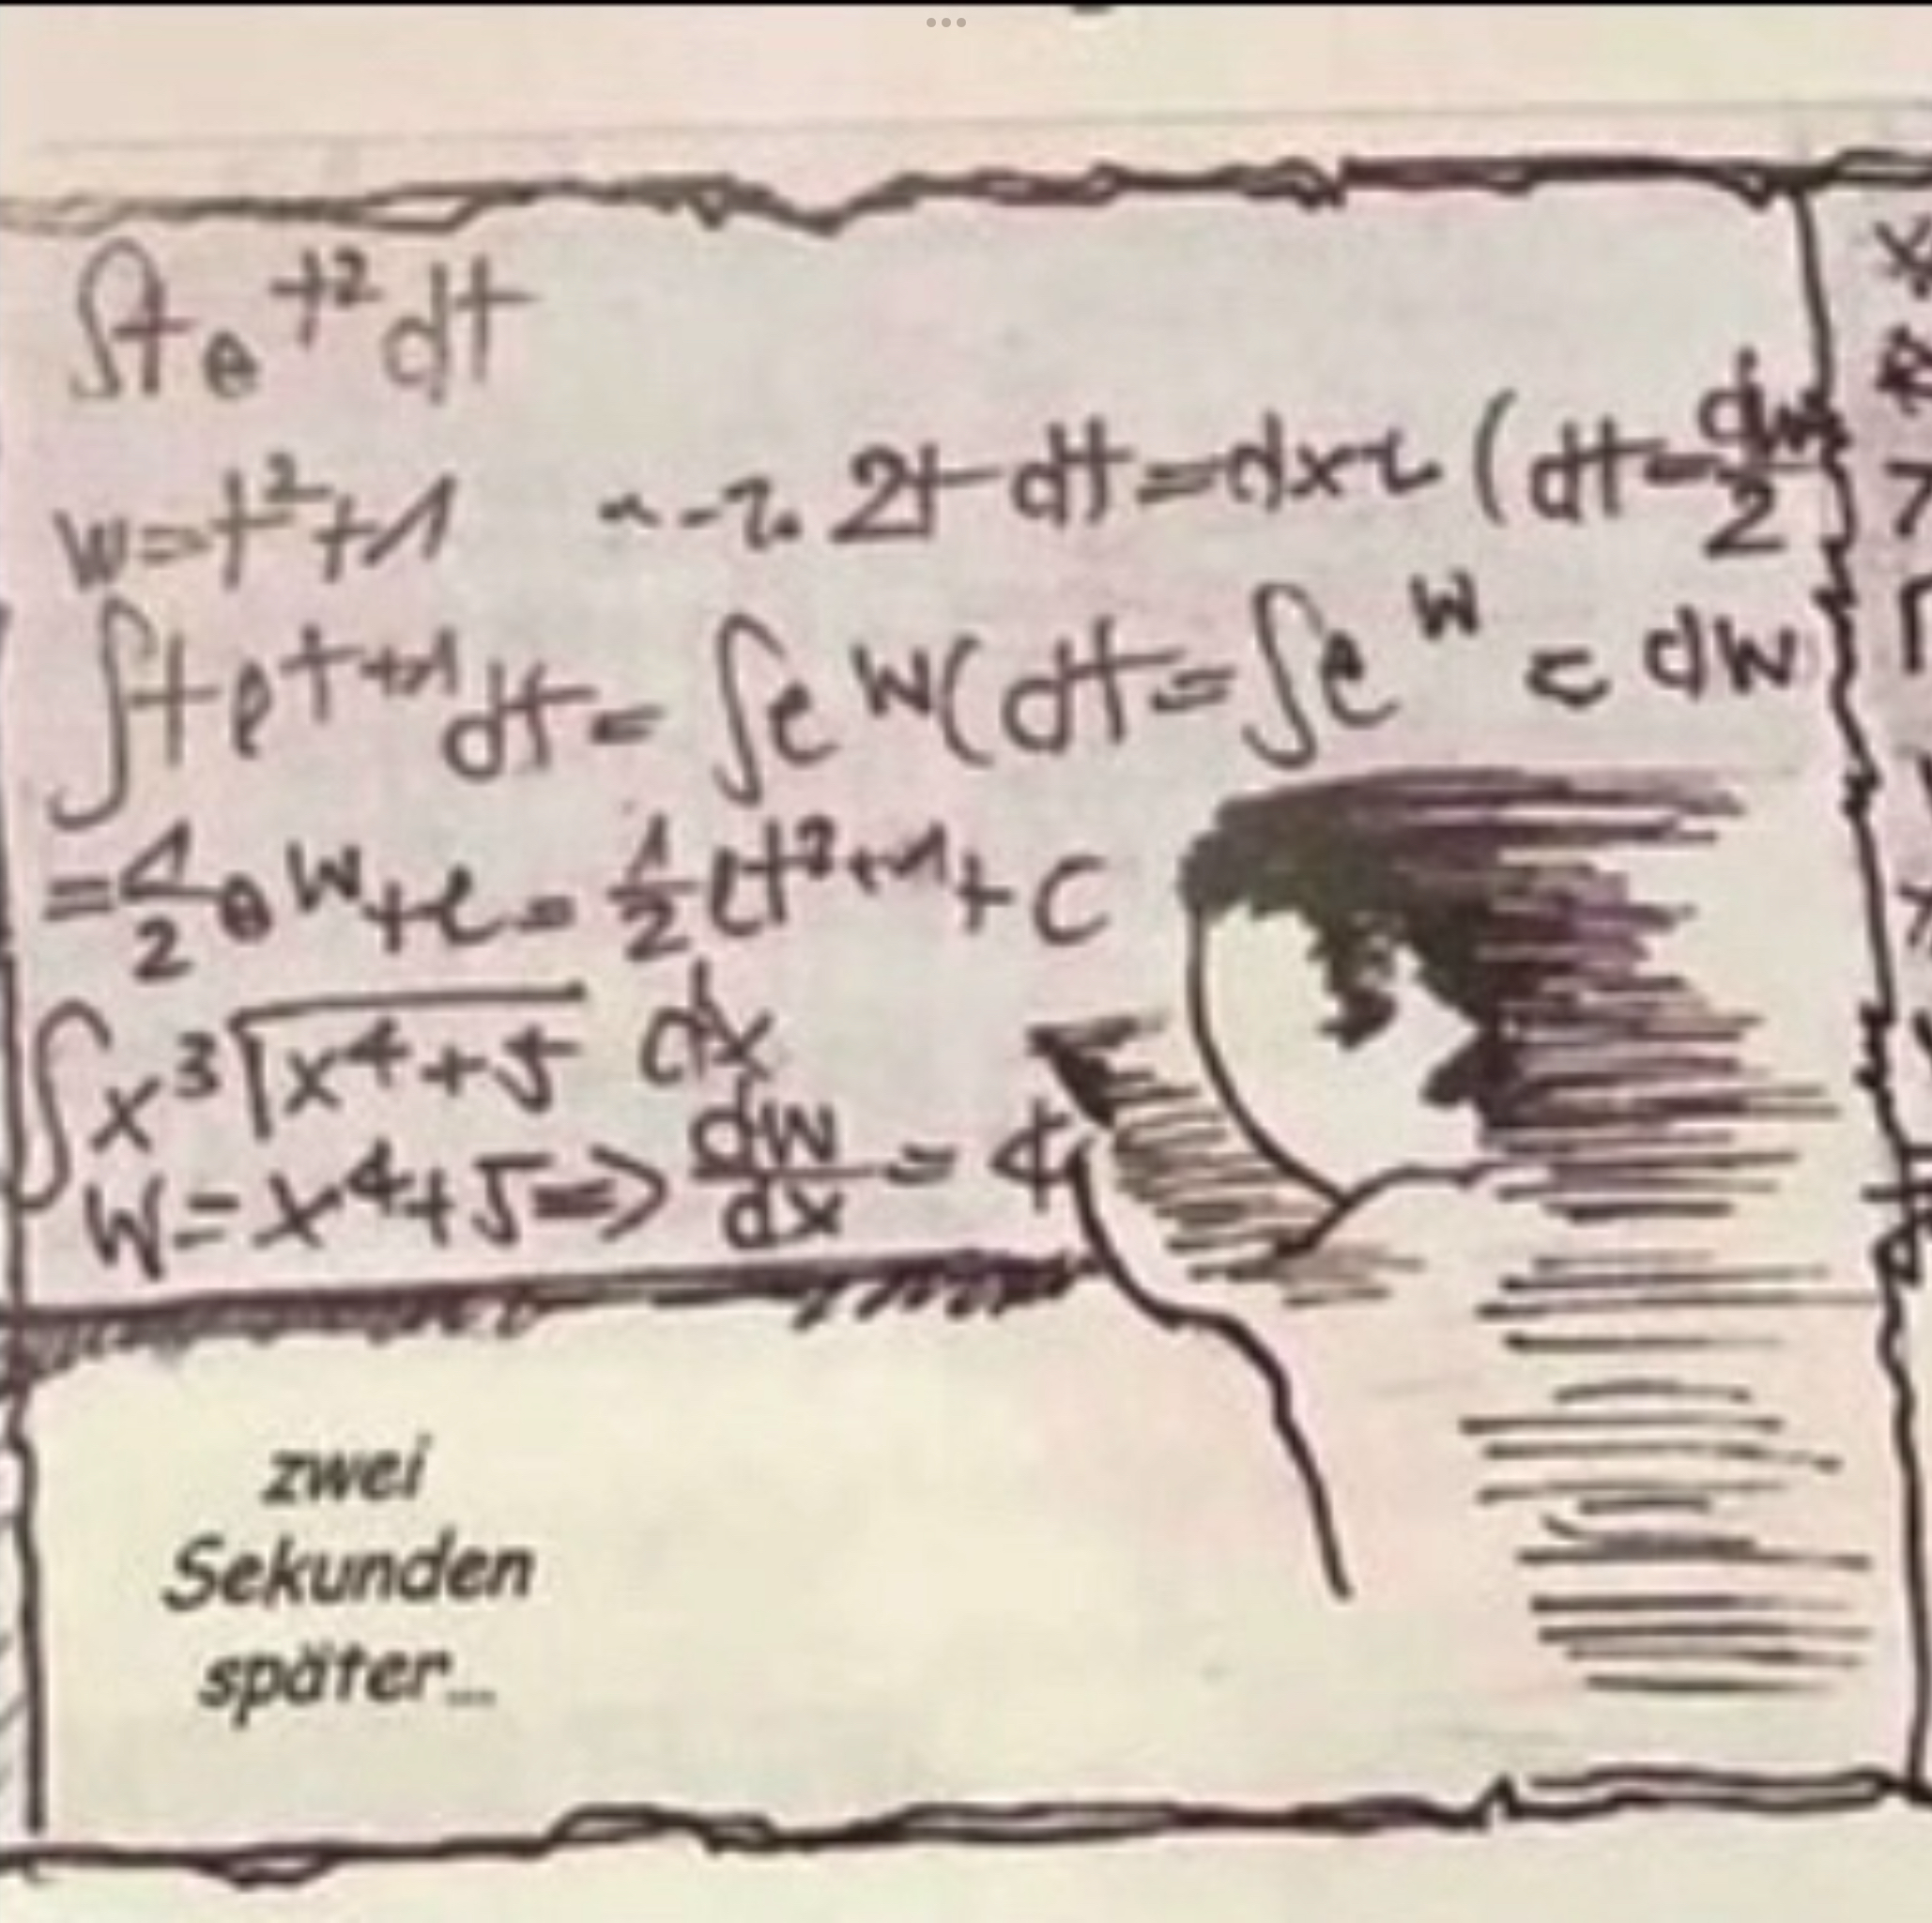
\includegraphics[width=1cm]{pictures/teacher_me_caricatur.png}}; % Adjust width and center image
\end{tikzpicture}}
}


\begin{document}
\maketitle
\thispagestyle{empty}
\cleardoublepage
\tableofcontents
\cleardoublepage

\pagestyle{headings}

\section{Einleitung}

\subsection{Probleme der Wahrscheinlichkeitsrechnung}

Die Wahrscheinlichkeitsrechnung --- so wie wir sie heute verstehen --- befasst sich mit der quantitativen Erfassung gewisser Aspekte zufälliger Ereignisse oder Beobachtungen. Was Zufall ist, wissen wir eigentlich nicht. Doch tritt dieses Phänomen in der Natur und in der sozialen Umwelt in Erscheinung.

In unserer unsicheren Welt hängen viele Dinge vom Zufall ab: Die Erbfaktoren bestimmen in der Vielfalt ihrer Kombinationen unseren Charakter und unser Aussehen, die Wahl des Ehepartners oder des Berufs wird oft durch eine zufällige Begegnung entschieden. Kleinigkeiten lösen Unfälle aus, die durch einen Zufall glimpflich oder tödlich verlaufen können, und eine plötzliche Eingebung hat schon manchem den grossen Gewinn im Lotto gebracht.

\begin{wrapfigure}{O}{0.382\textwidth}
  \centering
\includegraphics[width=0.35\textwidth]{pictures/tierknochen}
\caption{Antike Würfel}
\end{wrapfigure}
Ursprünglich war das Rechnen mit Wahrscheinlichkeiten ein Hilfsmittel für Glücksspiele (Würfelspiele, Kartenspiele, Roulette, Lotto etc.), die ja zu allen Zeiten und in allen Kulturen beliebt waren und es immer noch sind. Das Würfelspiel war sogar schon in der Antike weit verbreitet. Als Würfel verwendete man Tierknochen, sogenannte \emph{Astragale} (Sprungbeine von Schafen oder Ziegen).

Der eigentliche Beginn der klassischen Wahrscheinlichkeitsrechnung wird üblicherweise mit \textsc{Pierre de Fermat} (1601-1685) und \textsc{Blaise Pascal} (1623-1662) in Verbindung gebracht. Sie beschäftigten sich mit zwei jahrhundertelang ungelöst gebliebenen Problemen, die wir später in einer speziellen Aufgabe erörtern werden (Würfelproblem, Teilungsproblem). Eine lehrbuchartige Darstellung fand die Wahrscheinlichkeitsrechnung in dem 1713 erschienenen Buch \emph{De arte conjectandi} (etwa: Über die Kunst des Vermutens) des Schweizers \textsc{Jakob Bernoulli} (1655-1705).

In diesem Buch entwickelt \textsc{Bernoulli} zunächst die Kombinatorik und wendet diese dann auf Glücksspiele, aber auch auf wirtschaftliche Probleme an. Es enthält weiter das \emph{Gesetz der grossen Zahlen}, mit dem eine Verbindung zur Statistik hergestellt werden kann. Einen gewissen Abschluss erreichte die Wahrscheinlichkeitsrechnung in dem 1812 erschienenen Werk \emph{Théorie analytique des probabilités} von \textsc{Pierre Simon de Laplace} (1749-1827). Die Wahrscheinlichkeit wird dabei definiert als der Quotient aus der Anzahl der im Sinne der Fragestellung günstigen zur Anzahl der möglichen Ausgänge. An der Entwicklung der analytischen Methoden der Wahrscheinlichkeitsrechnung und der mathematischen Statistik waren ausser \textsc{Laplace} die folgenden Mathematiker beteiligt: \textsc{Abraham de Moivre} (1667-1754), \textsc{Carl Friedrich Gauss} (1777-1865), \textsc{Simeon Denis Poisson} (1781- 1840).
\begin{wrapfigure}{O}{0.4\textwidth}
\centering
\includegraphics[width=0.32\textwidth]{pictures/bernoulli}
\caption{\textsc{Daniel Ber\-noul\-li}}
\end{wrapfigure}

Die weitere Herausbildung der Wahrscheinlichkeitsrechnung als mathematische Disziplin ist insbesondere das Verdienst der russischen Mathematiker \textsc{Pafnuti Lwowitsch Tschebyschew} (1821- 1894), \textsc{Andrei Markow} (1856-1922), \textsc{Alexander Michailowitsch Ljapunow} (1857-1918) und \textsc{Andrei Kolmogorow} (1903-1989). Ihnen verdankt die Wahrscheinlichkeitsrechnung die Präzisierung einer Reihe wesentlicher Begriffsbildungen, insbesondere die axiomatische Erklärung des Wahrscheinlichkeitsbegriffs durch \textsc{Kolmogorow} im Jahre 1933. \textsc{Kolmogorow} verzichtet darauf zu sagen, wie man eine Wahrscheinlichkeit erhält; er legte bloss fest, wann eine reelle Zahl \glqq Wahrscheinlichkeit\grqq\ heissen darf und wie man mit diesen Zahlen dann rechnen kann.

Die modernen Naturwissenschaften sind ganz besonders auf Wahrscheinlichkeitsrechnungen angewiesen, zum Beispiel bei Problemen, die mit der Bewegung der Elementarteilchen zusammenhängen. Denn einzelne Teilchen bewegen sich in einer zufälligen Art, die nicht voraussehbar und nicht berechenbar ist. Moleküle treten aber praktisch immer in grossen Mengen auf, ihr kollektives Verhalten wird durch die Wahrscheinlichkeitsrechnung voraussehbar.

Mit den Methoden der Wahrscheinlichkeitsrechnung gelang es, zahlreiche Erscheinungen in einer der Realität noch besser angepassten Form mathematisch zu beschreiben, die schon erhaltenen Resultate zu interpretieren und auch zu neuen Erkenntnissen zu gelangen. Wahrscheinlichkeitstheorie und Statistik --- man nennt dies \emph{Stochastik} --- werden in Zukunft eine Schlüsselstellung einnehmen. Nur auf ihren Grundlagen können aufstrebende moderne, theoretisch anspruchsvolle und praktisch bedeutsame Theorien und Techniken verstanden werden. So wurden in den letzten Jahrzehnten mehrere Disziplinen entwickelt, die sich mit der Anwendung der Wahrscheinlichkeitsrechnung in verschiedenen Natur- und Gesellschaftswissenschaften, Medizin, Technik, Operation Research, Kybernetik und Ökonomie befassen, z.B. Bedienungstheorie, Zuverlässigkeitstheorie, Entscheidungstheorie, Nutzentheorie, Optionstheorie, Spieltheorie, Informationstheorie, statistische Qualitätstheorie, Monte-Carlo-Simulation oder Evolutionstheorie. Mit den heutigen Computern wächst die Anwendung von auf der Wahrscheinlichkeitsrechnung beruhenden Verfahren ständig. Zu den neusten Errungenschaften geh\"oren die Large Language Model und Machine Learning.

\subsection{Formalisierung}

\subsubsection{Zufallsversuche}
Mit Zufallsgeräten führt man Zufallsversuche durch, indem man die verschiedenen Aus\-gän\-ge oder Ergebnisse eines Zufallsexperiments beobachtet. Dabei versteht man unter einem \textbf{Zufallsversuch} einen --- zumindest theoretisch --- beliebig oft wiederholbaren Vorgang, dessen Ausgang sich nicht mit Sicherheit vorhersagen lässt.

\begin{itemize}
\item Zu Beginn eines Fussballspiels entscheidet eine Münze darüber, welche Mannschaft die Seitenwahl erhält.
\item Beim Spiel Backgammon entscheiden zwei Würfel darüber, wie viele Felder die Spielfiguren vorrücken dürfen.
\item Beim Einarmigen Banditen ist es nicht so offensichtlich, wie die einzelnen Walzen gesteuert werden. Man hat aber den Eindruck, dass sie zufällig über Gewinn und Verlust entscheiden.
\end{itemize}

\begin{cdef}[Stichprobenraum]
Die Menge aller möglichen Versuchsausgänge, $\omega_1, \omega_2, \dots, \omega_n$, eines Zufallsversuchs bezeichnet man als \textbf{Stichprobenraum} und bezeichnet diesen mit $\Omega$.
\end{cdef}

\begin{bsps}
F\"ur die Klassiker:
	\begin{itemize}
	\item Münze: $\omega_1:= $Kopf, $\omega_2:= $Zahl, also $\Omega=\set{\text{Kopf, Zahl}}$
	\item Würfel: $\Omega=\set{1,2,3,4,5,6}$
	\end{itemize}
\end{bsps}

\uebh{stichprobenraum}{
Bestimme einen geeigneten Stichprobenraum für den Versuch
	\begin{enumerate}[a)]
	\item Mit der Spitze eines Bleistifts wird blindlings auf eine Textseite eines Buches getippt; der getroffene Buchstabe wird notiert.
	\item Bei Familien mit drei Kindern wird festgestellt, ob die Kinder Jungen oder Mädchen sind.
	\end{enumerate}
}

\subsubsection{Ereignisse}
Wenn man beim Roulette auf \glqq impair\grqq\ setzt, ist man nicht so sehr daran interessiert, in welches Zahlenfach die Kugel fällt. Wichtig ist nur, ob das zufällige Ereignis eintritt, also die Kugel in eines der Fächer $1,3,5, \dots, 33, 35$ fällt. Diese  Ereignisse bilden eine Teilmenge $\mathbb{A}$ des Stichprobenraumes $\Omega=\set{0,1,2,3,\dots,35,36}$.

Mengen eignen sich hervorragend zur Beschreibung von Zufallsversuchen. Die Ausdrücke der Mengensprechweise werden lediglich in entsprechende Ausdrücke übertragen.

\begin{cdef}[Ereignis]
Bezeichne $\Omega$ einen Stichproberaum. Jede Teilmenge $\mathbb{A}\subset\Omega$ heisst ein \textbf{Ereignis}.
\end{cdef}

Endet eine Durchführung des Zufallversuchs mit dem Ausgang $\omega\in\mathbb{A}$, so sagt man: \glqq Das Ereignis $\mathbb{A}$ ist eingetreten.\grqq. Ist $\omega\not\in\mathbb{A}$, so sagt man: \glqq Das Ereignis $\mathbb{A}$ ist nicht eingetreten\grqq\ oder das \textbf{Gegenereignis} $\overline{\mathbb{A}} = \Omega\setminus\mathbb{A}$ ist eingetreten.

Da $\Omega$ alle möglichen Ereignisse enthält, tritt $\Omega$ bei jeder Durchführung des Versuchs ein. Man bezeichnet $\Omega$ deshalb auch als \textbf{das sichere Ereignis}. Da die leere Menge kein Element enthält, kann dieses Ereignis bei keiner Durchführung des Versuchs eintreten. Man bezeichnet $\emptyset$ deshalb auch als \textbf{das unmögliche Ereignis}. Beachten Sie $\overline{\Omega}=\Omega\setminus\Omega=\emptyset$ und  $\overline{\emptyset}=\Omega\setminus\emptyset=\Omega$; in Worten: das Gegenereignis vom sicheren Ereignis ist das unmögliche Ereignis und umgekehrt.

Sind $\mathbb{A}$ und $\mathbb{B}$ zwei Ereignisse desselben Zufallsversuchs und endet die Durchführung des Zufallversuchs mit dem Ausgang $\omega$, so sagt man,
\begin{itemize}
\item falls $\omega\in\mathbb{A}\cup\mathbb{B}$: \glqq Ereignis $\mathbb{A}$ \emph{oder} $\mathbb{B}$ ist eingetreten\grqq,
\item falls $\omega\in\mathbb{A}\cap\mathbb{B}$: \glqq Ereignis $\mathbb{A}$ \emph{und} $\mathbb{B}$ ist eingetreten\grqq.
\end{itemize}
Zwei Ereignisse $\mathbb{A}$ und $\mathbb{B}$ heissen \textbf{unvereinbar}, genau dann wenn sie nicht zugleich eintreten können, wenn also $\mathbb{A}\cap\mathbb{B}=\emptyset$ gilt.

\uebh{ereignisse}{
Bei einer Qualitätskontrolle werden drei produzierte Stücke der Reihe nach darauf untersucht, ob sie brauchbar (b) oder unbrauchbar (u) sind. Notiere folgende Ereignisse:
\begin{enumerate}[a)]
\item Das zweite Stück ist unbrauchbar.
\item Mindestens zwei Stücke sind unbrauchbar.
\end{enumerate}
}

\clearpage

\subsection{Notizen zu den \"Ubungen}

\begin{lsg}{stichprobenraum}
	\begin{enumerate}[a)]
	\item $\Omega=\{a,b,c,\dots,x,y,z,A,B,C,\dots,X,Y,Z\}$
	\item Stehe $w$ f\"ur M\"adchen und $m$ f\"ur Junge: $\Omega=\{www,wwm,wmm,mmm\}$
	\end{enumerate}
\end{lsg}

\begin{lsg}{ereignisse}
\begin{enumerate}[a)]
\item $\mathbb{U}=\{bub,buu,uub,uuu\}$
\item $\mathbb{M}=\{buu,uub,uuu\}$
\end{enumerate}
\end{lsg}

\clearpage

\section{Wahrscheinlichkeit}

\subsection{Das Gesetz der grossen Zahlen}

Für zwei Verspätungen hatte ein Arrestant $200$-mal einen Reissnagel zu werfen und zu notieren, ob er Stellung $0$ oder $1$ angenommen hat.
\begin{wrapfigure}{O}{0.382\textwidth}
\centering
\includegraphics[width=0.3\textwidth]{pictures/reisnagel}
\caption{Stellungen $0$ und $1$}
\end{wrapfigure}
Sein Ergebnisprotokoll siehst du in Tabelle \ref{tab:arrest} auf Seite \pageref{tab:arrest}.
\definecolor{lightyellow}{rgb}{1,1,0.8}
\definecolor{Gray}{gray}{0.9}
\begin{table}
\centering
\begin{tabular}{|l|c|c|c|c|c|c|} \hline
\rowcolor{Gray}\spaltenheight\# Würfe & 2 & 5 & 10 & 20 & 30 & 40\spaltensep \hline
\rowcolor{lightyellow}\spaltenheight$\nicefrac{\text{Einsen}}{\text{Würfe}}$ & 0 & 0.6 & 0.4 & 0.7 & 0.6 & 0.63\spaltensep \hline
\rowcolor{Gray}\spaltenheight\# Würfe & 60 & 80 & 100 & 120 & 140 & 160\spaltensep \hline
\rowcolor{lightyellow}\spaltenheight$\nicefrac{\text{Einsen}}{\text{Würfe}}$ & 0.67& 0.66 & 0.65 & 0.62 & 0.62 & 0.63\spaltensep \hline
\rowcolor{Gray}\spaltenheight\# Würfe & 180 & 200 & & & &\spaltensep \hline
\rowcolor{lightyellow}\spaltenheight$\nicefrac{\text{Einsen}}{\text{Würfe}}$ & 0.62 & 0.63 & & & &\spaltensep \hline
\end{tabular}
\caption{Anzahl Einsen zu Anzahl Würfen beim Reisnagel-Werfen}\label{tab:arrest}
\end{table}

\uebh{reissnagel}{
Stelle diese Daten graphisch in Abbildung \ref{graph} auf Seite \pageref{graph} dar.
}

\begin{figure}
\centering
\definecolor{cqcqcq}{rgb}{0.75,0.75,0.75}
\scalebox{1.1}{
\begin{tikzpicture}[line cap=round,line join=round,>=triangle 45,x=0.04cm,y=6.0cm]
\draw [color=cqcqcq,dash pattern=on 2pt off 2pt, xstep=0.8cm,ystep=1.2cm] (-2,-0.02) grid (205,1.05);
\draw[->,color=black] (-20,0) -- (220,0);
\foreach \x in {20,40,60,80,100,120,140,160,180,200}
\draw[shift={(\x,0)},color=black] (0pt,2pt) -- (0pt,-2pt) node[below] {\footnotesize $\x$};
\draw[color=black] (205.46,0.01) node [anchor=south west] { \# Würfe};
\draw[->,color=black] (0,-0.1) -- (0,1.2);
\foreach \y in {,0.2,0.4,0.6,0.8,1}
\draw[shift={(0,\y)},color=black] (2pt,0pt) -- (-2pt,0pt) node[left] {\footnotesize $\y$};
\draw[color=black] (1.32,1.14) node [anchor=west] { $\nicefrac{\text{\#Einsen}}{\text{\#Würfe}}$};
\clip(-20,-0.2) rectangle (220,1.2);
\end{tikzpicture}
}
\caption{Grid zur Darstellung des Reiss\-nagel-\-Versuchs}\label{graph}
\end{figure}

Nach anfänglichen Schwankungen stabilisiert sich der Wert für die relative Häufigkeit der Ziffer $1$, also die Anzahl Einsen/Anzahl Würfe, um den Wert $0.625$ herum. Die Wahrscheinlichkeiten \glqq pendeln sich ein\grqq.

Auf Grund dieses Beispiels liegt es nahe, jedem Ausgang $\omega$ eines Zufallversuchs eine Wahrscheinlichkeit $P(\omega)$ zuzuordnen. Diese Wahrscheinlichkeit steht für den festen Wert, auf den sich die relative Häufigkeit des betreffenden Ausgangs einpendelt, wenn der Versuch öfter wiederholt wird. Beim Reissnagel wurden diese Werte $P(1)\approx0.625$ und $P(0)\approx0.375$ empirisch durch Experimente ermittelt. Bei anderen Zufallsgeräten kann man die Wahrscheinlichkeit oft auf Grund ihrer Symmetrie oder Geometrie angeben.

\begin{bem}
Die Bezeichnung $P$ lehnt sich ans Englische Probability.
\end{bem}

Die \emph{relative Häufigkeit} ist eine experimentelle Messung der mathematischen Wahrscheinlichkeit. Der Wahrscheinlichkeitsbegriff ist dadurch als statistischer Begriff charakterisiert. Die Wahrscheinlichkeit, auf dem Mars lebendige Wesen anzutreffen, oder die Wahrscheinlichkeit, dass Cäsar in Grossbritannien war, entsprechen nicht unserem Wahrscheinlichkeitsbegriff, da er bei diesen Beispielen im qualitativen Sinn verwendet wird. Verlangt wird jedoch ein quantitativer Wahrscheinlichkeitsbegriff. Man kann nicht, wie es sonst in der Mathematik üblich ist, durch Rückführung auf andere Begriffe streng definieren, was man unter der Wahrscheinlichkeit eines Ergebnisses oder Ereignisses versteht. Denn die Wahrscheinlichkeit eines Ergebnisses oder Ereignisses ist eine auf Erfahrungen beruhende Annahme. Deshalb ist es ohne zusätzliche Annahmen nicht möglich, den Zahlenwert für eine Wahrscheinlichkeit exakt zu ermitteln. Dennoch ist dieses Vorgehen gerechtfertigt, weil die so aufgebaute Wahrscheinlichkeitsrechnung sich bei zahllosen Anwendungen in den verschiedensten Gebieten glänzend bewährt hat und Vorhersagen, die man aufgrund wahrscheinlichkeitstheoretischer Überlegungen über zukünftige Ereignisse gemacht hat, sich immer wieder bestätigt haben.

\subsection{Laplace'sche Definition einer Wahrscheinlichkeit}

Nachdem jedem Ausgang $\omega$ eines Zufallversuchs auf plausible Weise ein Wert als Wahrscheinlichkeit zugeordnet werden konnte, definieren wir für ein Ereignis $\omega$ entsprechend die zugehörige Wahrscheinlichkeit $P(\omega)$.

\begin{cdef}[Wahrscheinlichkeit eines Ereignisses]
$P(\omega)$ ist gleich der Summe der Wahrscheinlichkeiten aller Ausgänge in $\mathbb{A}$.
\end{cdef}

\begin{bsps}
Es ist eine gute Idee, sich an klassischen Beispielen zu orientieren.
\begin{itemize}
\item Wie gross ist die Wahrscheinlichkeit, mit einem Würfel eine ungerade Zahl zu werfen?
Ereignis $\mathbb{A}=\setm{\omega}{\omega\text{ ist ungerade}}=\set{1,3,5}$, also $P(\mathbb{A})=\frac{1}{6}+\frac{1}{6}+\frac{1}{6}=\frac{1}{2}$.
\item Wie gross ist die Wahrscheinlichkeit, aus einem Jasskartenspiel einen Buben zu ziehen?
$P(\mathbb{A})=\frac{1}{36}+\frac{1}{36}+\frac{1}{36}+\frac{1}{36}=\frac{1}{9}$
\end{itemize}
\end{bsps}

\begin{bem}
Für die Sonderfälle, sicheres und unm\"ogliches Ereignis, gilt:
$$P(\Omega)=1\q\text{und}\q P(\emptyset)=0.$$
\end{bem}

\uebh{kopfoderzahl}{
Wie gross ist die Wahrscheinlichkeit bei einem Wurf
\begin{enumerate}[a)]
\item mit einer Münze Kopf, Kopf oder Zahl, Kopf und Zahl,
\item mit einem Würfel eine 3, eine Quadratzahl
\end{enumerate}
zu werfen?
}

\uebh{geburtenregel}{
In England gab es im Zeitraum von 1938-1947 6620794 Einzel-, 81133 Zwillings-, 667 Drillings- und 14 Vierlingsgeburten. Überprüfe die in der Gy\-nä\-ko\-lo\-gie übliche Regel:
\begin{quote}
Ist $p$ die ungefähre Wahrscheinlichkeit für eine Zwillingsgeburt, so ist $p^2$ die ungefähre Wahrscheinlichkeit für eine Drillingsgeburt und $p^3$ die ungefähre Wahrscheinlichkeit für eine Vierlingsgeburt.
\end{quote}
}

Ausgehend von der Erfahrung, dass die relativen Häufigkeiten eines Ereignisses $\mathbb{A}$ bei fortgesetzter Wiederholung eines Zufallversuchs einem bestimmten Wert zustreben, fasste \textsc{Richard von Mises} (1883-1953) die Wahrscheinlichkeit von $\mathbb{A}$ als Grenzwert der relativen Häufigkeiten bei unbegrenzter Wiederholung eines Zufallversuchs auf. Dies war die statistische Definition der Wahrscheinlichkeit.

\subsection{Definition nach Kolmogorov}

\begin{figure}
\centering
\includegraphics[width=0.5\textwidth]{pictures/kolmogorov}
\caption{\textsc{Andrey Kolmogorov}}
\end{figure}

In dem weiteren Aufbau der Wahrscheinlichkeitstheorie erwies sich diese Definition als ungeeignet, da unüberwindliche Schwierigkeiten auftraten. Der uns bekannte Limesbegriff im Sinne der Analysis lässt sich nämlich nicht auf eine vom Zufall beherrschte Folge anwenden, in der immer wieder \glqq Ausreisser\grqq\ möglich sind. Eine logisch befriedigende Fassung des Wahrscheinlichkeitsbegriffs wurde erst durch den Verzicht auf eine direkte Definition möglich. \textsc{Kolmogorow} forderte lediglich gewisse Eigenschaften für Wahrscheinlichkeiten und zeigte 1933, dass sich bereits aus wenigen Axiomen eine Wahrscheinlichkeitstheorie entwickeln lässt.

\begin{cdef}[Wahrscheinlichkeit nach Kolmogorov]
Ist
\marginnote{
\qrcode{
https://www.youtube.com/watch?v=LGmmqxRnRCg}
}
$P$ eine Funktion, die jedem Ereignis $\mathbb{A}$ eines Stichprobenraumes $\Omega$ genau eine reelle Zahl $P(\mathbb{A})$ zuordnet, so heisst $P$ eine \emph{Wahrscheinlichkeitsfunktion} und jeder Funktionswert $P(\mathbb{A})$ die \emph{Wahrscheinlichkeit} von $\mathbb{A}$, genau dann, wenn folgende (Kolmogorow-)Axiome erfüllt sind:
\begin{itemize}
\item $P(\mathbb{A})\geq0, \forall\mathbb{A}\subset\Omega$ \hfill(Positivität)
\item $P(\Omega)=1$ \hfill(Normierung)
\item $\forall\mathbb{A},\mathbb{B}\subset\Omega$ mit $\mathbb{A}\cap\mathbb{B}=\emptyset\implies P(\mathbb{A}\cup\mathbb{B})=P(\mathbb{A})+P(\mathbb{B})$ \hfill(Additivität)
\end{itemize}
\end{cdef}

Aus den Axiomen folgert man sofort
\begin{csatz}[Gegenwahrscheinlichkeit]
Mit
\marginnote{
\qrcode{
https://youtu.be/Yb8tCa24Gi8}
}
den üblichen Bezeichnungen gilt
$$P(\overline{\mathbb{A}})=1-P(\mathbb{A}).$$
\end{csatz}
\begin{proof}[Beweis]
Wegen $\mathbb{A}\cap\overline{\mathbb{A}}=\emptyset$ und $\mathbb{A}\cup\overline{\mathbb{A}}=\Omega$ gilt
$$1=P(\Omega)=P(\mathbb{A}\cup\overline{\mathbb{A}})=P(\mathbb{A})+P(\overline{\mathbb{A}}),$$
also $P(\overline{\mathbb{A}})=1-P(\mathbb{A})$.
\end{proof}

\begin{bsp}
Ein illustratives Beispiel für eine Anwendung ist die Suche nach der Antwort auf die Frage:
\begin{quote}
Mit einem fairen Spielw\"urfel: Wie gross ist die Wahrscheinlichkeit in $10$ Würfen mindestens einmal eine $6$ zu werfen?
\end{quote}
Dies zu berechnen ist ziemlich aufwändig. Denn man muss die Wahrscheinlichkeit berechnen, genau $1$-mal eine $6$, genau $2$-mal eine $6$, \dots, genau $10$-mal eine $6$ in $10$ Würfen zu realisieren; danach muss man noch die einzelnen Wahrscheinlichkeiten aufsummieren. Zudem ist die Berechnung der einzelnen Wahrscheinlichkeiten --- beispielsweise genau $3$ $6$en in $10$ Würfen --- nicht trivial (Resultat $15.5\%$).

Einfacher geht es über das Gegenereignis von \glqq mindestens $1$-mal eine $6$ zu werfen\grqq; das ist nämlich \glqq nie eine $6$ in $10$ Würfen\grqq\ zu erzielen. Es ist
$$P(\text{keine $6$ in $10$ Würfen})=\left(\frac{5}{6}\right)^{10}\approx0.1615.$$
Nun kann man mit obigem Satz einfach schliessen, dass die Wahrscheinlichkeit \glqq in $10$ Würfen mindestens einmal eine $6$\grqq\ zu würfeln
\begin{align*}
P(\text{mindestens eine $6$ in $10$ Würfen}) & = 1-P(\text{keine $6$ in $10$ Würfen})\\
& \approx1-0.1615=0.8385\approx84\%,
\end{align*}
sein muss.
\end{bsp}

\begin{bem}
Die Beziehung aus obigem Satz wird sehr oft benötigt, da in vielen Fällen die Wahrscheinlichkeit des Gegenereignisses $\overline{\mathbb{A}}$ leichter zu berechnen ist als die Wahrscheinlichkeit des Ereignisses $\mathbb{A}$.
\end{bem}

\begin{csatz}[günstig durch möglich]
Hat ein Zufallsversuch $n$ mögliche Ausfälle $\omega_1, \omega_2, \omega_3, \dots, \omega_n$ und ist jeder dieser Ausfälle gleich wahrscheinlich, also $P(\omega_i)=\frac{1}{n}$, so gilt für ein Ereignis $\mathbb{A}$
$$P(\mathbb{A})=\frac{1}{n}+\frac{1}{n}+\dots+\frac{1}{n}=\frac{\card(\mathbb{A})}{\card(\Omega)}.$$
\end{csatz}
\begin{proof}[Beweis]
Brauche Kol\-mo\-go\-rof-Ad\-di\-ti\-vi\-tät.
\end{proof}

\begin{cdef}[Klassische Wahrscheinlichkeit nach Laplace]
In obigem Fall gilt also für die Wahrscheinlichkeit eines Ereignisses $\mathbb{A}$: Anzahl der günstigen Fälle für $\mathbb{A}$ geteilt durch Anzahl der möglichen Fälle $\Omega$, oder kurz
$$P(\mathbb{A}):=\frac{|\mathbb{A}|}{|\Omega|}=\frac{g}{m}.$$
\end{cdef}

\begin{bsps}
Würfeln mit einem fairen Spielwürfel, Ziehen von Losen aus einer gut durchmischten Urne, Ziehen von Karten aus einem gut durchmischten Kartenspiel etc.
\end{bsps}

Die letzte Folgerung aus den Axiomen entspricht der klassischen Definition der Wahrscheinlichkeit, die von Laplace stammt. Diese Definition hat den Nachteil, dass man sich auf endlich viele Ereignisse, die alle noch gleich wahrscheinlich sein müssen, beschränken muss. Der axiomatische Aufbau der Wahrscheinlichkeitsrechnung wird heute in der Mathematik allgemein benutzt, weil man nicht mehr den Einschränkungen unterworfen und die klassische Definition als Sonderfall enthalten ist.

\uebh{energiearten}{
In einer Stadt werden von allen Gebäuden 15\% elektrisch, 35\% mit Öl, 25\% mit Kohle und der Rest mit Erdgas beheizt. Wie gross ist die Wahrscheinlichkeit, dass ein zufällig ausgewähltes Gebäude
\begin{enumerate}[a)]
\item mit Kohle,	
\item nicht mit Öl,
\item weder mit Kohle noch mit Öl beheizt wird?
\end{enumerate}
}

\uebh{hundertkugeln}{
Eine Urne enthält 100 Kugeln mit den Nummern $00,01,02,$ \dots $,98,99$. Eine Kugel wird zufällig gezogen. Es sei $X$ die erste und $Y$ die zweite Ziffer ihrer Nummer. Berechne die Wahrscheinlichkeiten $P(X = 3)$, $P(Y\neq 4)$, $P(X \neq Y)$, $P(X < 4\text{ und } Y < 3)$ und $P(X\cdot Y > 49)$.
}

\uebh{pferderennen}{
Die Pferde Artemis, Borodir, Condor und Durin bestreiten ein Galopprennen. Die Wahrscheinlichkeit, dass A gewinnt, ist doppelt so gross wie die von B, und die von B ist doppelt so gross wie die von C. Die Wahrscheinlichkeit, dass D gewinnt, ist dreimal so gross wie die von C. Wie gross ist die Wahrscheinlichkeit, dass

\begin{minipage}{3.8cm}
\begin{enumerate}[a)]
\item A,
\item B,
\end{enumerate}
\end{minipage}
\begin{minipage}{3.9cm}
\begin{enumerate}[a)]
\addtocounter{enumi}{2}
\item C,
\item B oder C gewinnt?
\end{enumerate}
\end{minipage}

Beim Aufgalopp verletzt sich Borodir und kann deshalb am Rennen nicht teilnehmen. Wie gross
ist jetzt die Wahrscheinlichkeit, dass D gewinnt?
}

\uebh{bauersucht}{
Ein Bauer erfährt, dass auf seinem $\unit[60]{m} \times \unit[40]{m}$ grossen Acker irgendwo ein Schatz vergraben ist. Wie gross ist die Wahrscheinlichkeit, dass der Schatz

\begin{enumerate}[a)]
\item mindestens zehn Meter von der Mitte entfernt ist?
\item gefunden wird, wenn man zehn Löcher mit einem
Durchmesser von $\unit[10]{m}$ gräbt?
\item Wie viele Löcher vom gleichen Durchmesser müsste man graben, um mit mindestens $80$-prozentiger Sicherheit den Schatz zu finden?
\end{enumerate}

Hinweis: In diese Aufgabe handelt es sich um geometrische Wahrscheinlichkeiten, definiert durch das Verhältnis des Inhalts der günstigen Fläche zum Inhalt der möglichen Fläche. Auch diese Zuordnung erfüllt die drei Axiome von Kolmogorow, ist also eine Wahrscheinlichkeit.
}

\clearpage

\subsection{Notizen zu den \"Ubungen}

\begin{lsg}{reissnagel}
Der Plot sieht vielleicht so aus:

\definecolor{cqcqcq}{rgb}{0.75,0.75,0.75}
\definecolor{darkgreen}{rgb}{0.0,0.5,0.0}
\scalebox{0.618}{
\begin{tikzpicture}[line cap=round,line join=round,>=triangle 45,x=0.04cm,y=6.0cm]
\draw [color=cqcqcq,dash pattern=on 2pt off 2pt, xstep=0.8cm,ystep=1.2cm] (-2,-0.02) grid (205,1.05);
\draw[->,color=black] (-20,0) -- (220,0);
\foreach \x in {20,40,60,80,100,120,140,160,180,200}
\draw[shift={(\x,0)},color=black] (0pt,2pt) -- (0pt,-2pt) node[below] {\footnotesize $\x$};
\draw[color=black] (205.46,0.01) node [anchor=south west] { \# Würfe};
\draw[->,color=black] (0,-0.1) -- (0,1.2);
\foreach \y in {,0.2,0.4,0.6,0.8,1}
\draw[shift={(0,\y)},color=black] (2pt,0pt) -- (-2pt,0pt) node[left] {\footnotesize $\y$};
\draw[color=black] (1.32,1.14) node [anchor=west] { $\nicefrac{\text{\#Einsen}}{\text{\#Würfe}}$};
% Draw points
	\def\pointradius{3pt}
    \fill[darkgreen] (2,0) circle (\pointradius);
    \fill[darkgreen] (5,0.6) circle (\pointradius);
    \fill[darkgreen] (10,0.4) circle (\pointradius);
    \fill[darkgreen] (20,0.7) circle (\pointradius);
    \fill[darkgreen] (30,0.6) circle (\pointradius);
    \fill[darkgreen] (40,0.63) circle (\pointradius);
    \fill[darkgreen] (60,0.67) circle (\pointradius);
    \fill[darkgreen] (80,0.66) circle (\pointradius);
    \fill[darkgreen] (100,0.65) circle (\pointradius);
    \fill[darkgreen] (120,0.62) circle (\pointradius);
    \fill[darkgreen] (140,0.62) circle (\pointradius);
    \fill[darkgreen] (160,0.63) circle (\pointradius);
    \fill[darkgreen] (180,0.62) circle (\pointradius);
    \fill[darkgreen] (200,0.63) circle (\pointradius);
\clip(-20,-0.2) rectangle (220,1.2);
\end{tikzpicture}
}
\end{lsg}

\begin{lsg}{kopfoderzahl}
\begin{enumerate}[a)]
\item Mit den intuitiv verständlichen Abkürzungen haben wir $P(K)=\frac{1}{2}$, $P(K\cup Z)=1$ und $P(K\cap Z)=0$.
\item $P(3)=\frac{1}{6}$ bzw. $P(QZ)=\frac{2}{6}=\frac{1}{3}$
\end{enumerate}
\end{lsg}

\begin{lsg}{geburtenregel}
Die aufgef\"uhrten Geburten addieren sich zu $m=6\,702\,608$. Also erhalten wir als Wahrscheinlichkeit f\"ur eine Zwillingsgeburt $p=\frac{81133}{m}\approx0.0121$ und daraus folgt $p^{2}\approx0.000147$ sowie $p^{3}\approx0.00000177$, was wir vergleichen mit $P(3ling)=\frac{667}{m}\approx0.0000995$ und $P(4ling)=\frac{14}{m}\approx0.0000021$.
\end{lsg}

\begin{lsg}{energiearten}
Wir lassen Prozente weg und rechnen:
\begin{enumerate}
\item $P(K)=\frac{25}{100}=\frac{1}{4}$
\item $P(O)=\frac{7}{20}\implies P(\overline{O})=1-P(O)=\frac{13}{20}$
\item $P(\overline{K\cup O})=1-\frac{3}{5}=\frac{2}{5}$
\end{enumerate}
\end{lsg}

\begin{lsg}{hundertkugeln}
Eins nach dem andern
\begin{enumerate}[a)]
\item $P(X=3)=\frac{10}{100}=\frac{1}{10}$
\item $P(Y\neq4)=\frac{90}{100}=\frac{9}{10}$
\item $P(Y\neq4)=\frac{90}{100}=\frac{9}{10}$
\item $P(X \neq Y)=\frac{10\cdot9}{100}=\frac{9}{10}$
\item $P(X < 4\text{ und } Y < 3)=\frac{4\cdot 3}{100}=\frac{3}{25}$
\item Man z\"ahlt alle g\"ultigen Produkte und teilt durch die m\"oglichen F\"alle: $P(X\cdot Y > 49)=\frac{1+2+3+4}{100}=\frac{1}{10}$
\end{enumerate}
\end{lsg}

\begin{lsg}{pferderennen}
Zuerst kann man mit Dreisatz die Verh\"altnisse der Siegeswahrscheinlichkeiten der Pferde bestimmen. Wir erhalten $P(A)=\frac{4}{10}$, $P(B)=\frac{2}{10}$, $P(C)=\frac{1}{10}$ und $P(D)=\frac{3}{10}$. Damit sind die ersten drei Teilaufgaben gegessen. Ferner ist $P(B\cup C)=\frac{3}{10}$. Wenn B nicht mittun kann, dann ist $P(D)=\frac{3}{8}$.
\end{lsg}

\begin{lsg}{bauersucht}
Die Gesamtfl\"ache, die den m\"oglichen Fundort enth\"alt, betr\"agt $A=\unit[2400]{m^{2}}$.
\begin{enumerate}[a)]
\item Der Bereich um $\unit[10]{m}$ um die Mitte betr\"agt $M=\unit[100\pi]{m^{2}}$. Also $P(\overline{M})=1-\frac{M}{A}\approx0.87$.
\item Wenn man nicht wild drauf los gr\"abt, so \"uberschneiden sich die L\"ocher paarweise nicht. Dann kriegt man $P(10)=\frac{10\cdot25\pi}{A}\approx0.33$
\item Sei $d$ der Durchmesser und $x$ die Anzahl L\"ocher. Es ist:
\begin{align*}
x\cdot\frac{(\frac{d}{2})^{2}\pi}{2400} &\geq80\%\\
x\cdot\frac{d^{2}\pi}{9600} &\geq80\%\\
x &\geq 0.8\cdot\frac{9600}{d^{2}\pi}
\end{align*}
F\"ur den Durchmesser $d=\unit[10]{m}$ von oben erh\"alt man $x\geq24.45$. D.h man m\"usste mindestens 25 L\"ocher graben, um mit einer Wahrscheinlichkeit von mehr als $80\%$ den Schatz zu finden.
\end{enumerate}
\end{lsg}

\clearpage

\section{Stochastische Prozesse}

\subsection{Wahrscheinlihckeitsbaum}

Im vorherigen Kapitel haben wir einstufige Zufallsversuche betrachtet: Der Zufallsversuch wurde nur einmal durchgeführt. \emph{Stochastische} (griech., zufällige) \emph{Prozesse} sind eine Folge von einstufigen Versuchen, also mehrstufige Zufallsversuche. Dabei kann der Ausgang auf einer bestimmten Stufe durchaus vom Ausgang der vorherigen Stufen abhängen. Der Ablauf eines stochastischen Prozesses kann in den meisten Fällen übersichtlich durch ein Baumdiagramm dargestellt werden.

\begin{bsp}
Aus
\marginnote{
\qrcode{
https://youtu.be/sb4FPdTdXcU}
}
einer Urne mit drei roten und zwei grünen Kugeln wird eine Kugel gezogen und ihre Farbe notiert. Danach wird die Kugel wieder zurückgelegt und der Versuch wiederholt.
Hier hängt die zweite Stufe nicht vom Ausgang der ersten Stufe ab. Der zugehörige Stichprobenraum ist $\Omega=\set{rr, rg, gr, gg}$.
Die Figur \ref{fig:baum} auf Seite \pageref{fig:baum} zeigt das Baumdiagramm dieses stochastischen Prozesses.

\begin{figure}[h!]
\centering

\tikzset{
zahl/.style={fill=green!70!yellow, text=black, label=center:\textsf{\Large g}},
kopf/.style={fill=red!70!yellow, label=center:\textsf{\Large r}}
}
\begin{tikzpicture}
[scale=1.2, transform shape, 
thick,
every node/.style={draw, circle, minimum size=8mm},
grow=down,  %Zeichenrichtung
level 1/.style={sibling distance=4cm},
level 2/.style={sibling distance=2.5cm}, 
%level 3/.style={sibling distance=2cm}, 
level distance=1.75cm]

%\node[fill=gray!20, shape=rectangle, rounded corners, minimum width = 6cm] {Urne mit 3 roten und 2 grünen Kugeln} 

%child{
\node[shape=circle split,draw,line width=1pt,minimum size=8mm,inner sep=0mm, font=\sffamily\normalsize, rotate=30]  (Start) { \rotatebox{-30}{3r} \nodepart{lower}  \rotatebox{-30}{2g}}
 child {node[kopf] (A) {}
         child {node[kopf] (B) {}}
        child {node[zahl] (C) {}}
}
 child {node[zahl] (D) {}
          child {node[kopf] (E) {}}
          child {node[zahl] (F) {}}
};

%Füllung der Wurzel = "Start"
\begin{scope}[on background layer, rotate=30]
    \fill[kopf] (Start.base) ([xshift=0mm]Start.east) arc (0:180:5.5mm)--cycle;
    \fill[zahl] (Start.base) ([xshift= 0pt]Start.west) arc (180:360:5.5mm)--cycle;  
\end{scope}

%Beschriftung
\path (Start) -- (A) node [draw=none,  near start, left] {$\frac{3}{5}$};
\path (A) -- (B) node [draw=none,  near start, left] {$\frac{3}{5}$};
\path (A) -- (C) node [draw=none,  near start, right] {$\frac{2}{5}$};
\path (Start) -- (D) node [draw=none,  near start, right] {$\frac{2}{5}$};
\path (D) -- (E) node [draw=none,  near start, left] {$\frac{3}{5}$};
\path (D) -- (F) node [draw=none,  near start, right] {$\frac{2}{5}$};
%
\node[below=11pt, draw=none] at (B) {$\frac{9}{25}$};
\node[below=11pt, draw=none, name=X] at (C) {$\frac{6}{25}$};
\node[below=11pt, draw=none, name=Y] at (E) {$\frac{6}{25}$};
\node[below=11pt, draw=none] at (F) {$\frac{4}{25}$};
%
\draw[densely dashed, rounded corners, thin] (X.south west) rectangle (Y.north east);

\end{tikzpicture}


\caption{Wahrscheinlichkeitsbaum für die Urne (mit Zurücklegen)}\label{fig:baum}
\end{figure}

Jedem Ausgang entspricht ein Pfad durch den Baum. Die Zweige der Pfade sind mit entsprechenden Wahrscheinlichkeiten belegt. Beachten Sie, dass die Wahrscheinlichkeiten der Zweige, die von einem Knoten ausgehen, zusammen $1$ ergeben.

Um eine vernünftige Definition für die Wahrscheinlichkeit eines Pfades zu finden, stellt man sich vor, dass dieser zweistufige Prozess $N$-mal abläuft, wobei $N$ eine grosse Zahl, z.B. $10000$, bedeutet. In $\nicefrac{3}{5}$ der $N$ Wiederholungen wird man zu dem Knoten $r$ gelangen, also etwa $6000$ mal. $\nicefrac{2}{5}$ dieser $\nicefrac{3}{5}$ $N$ Fälle führen von $r$ zu $g$; der Pfad $rg$ wird also etwa $2400$ mal durchlaufen. Die Wahrscheinlichkeit für diesen Pfad ist somit
$$\frac{\frac{2}{5}\cdot\frac{3}{5}\cdot N}{N}=\frac{6}{25}.$$
\end{bsp}

\begin{csatz}[Pfadwahrscheinlichkeit]{}
Die Wahrscheinlichkeit eines Pfades ist gleich dem Produkt aller Wahrscheinlichkeiten längs des Pfades.
\end{csatz}
\begin{proof}[Beweis]
Den Beweis führt man wie oben im Beispiel, aber mit Variablen.
\end{proof}

\begin{ueb}[Kugel ziehen ohne Zurücklegen]
Berechne die entsprechenden Wahrscheinlichkeiten für den stochastischen Prozess, bei dem die zuerst gezogene Kugel nicht zurückgelegt wird. Zeichne das zugehörige Baumdiagramm.
\end{ueb}

\begin{ueb}[Anna aus Ananas]
Aus der Urne $\set{A, N, A, N, A, S}$ werden vier Buchstaben nacheinander ohne Zurücklegen zufällig gezogen. Wie gross ist die Wahrscheinlichkeit, das Wort \glqq ANNA\grqq\ zu erhalten? Zeichne auch ein Baumdiagramm.
\end{ueb}

\begin{ueb}[Meteo]
Für Wetterprognosen in Therwil gelten die Regeln: Wenn es heute trocken ist, dann ist es morgen mit der Wahrscheinlichkeit $\nicefrac{5}{6}$ wieder trocken. Wenn es heute regnet, dann regnet es morgen mit der Wahrscheinlichkeit $\nicefrac{2}{3}$. Heute ist Sonntag, und es ist trocken. Wie gross ist die Wahrscheinlichkeit, dass es am
\begin{enumerate}[a)]
\item Montag regnet,
\item Dienstag trocken ist,
\item Mittwoch regnet,
\item Donnerstag trocken ist?
\end{enumerate}

Zeichne ein Baumdiagramm.
\end{ueb}

\subsection{Unendliche Prozesse}

\begin{ueb}[Schuss auf Ziel]
\ \\[-4ex]
\begin{enumerate}[a)]
\item Stan und Oliver schiessen gleichzeitig auf dasselbe Ziel. Die Trefferwahrscheinlichkeiten sind 80\% bzw. 70\%. Wie gross ist die Wahrscheinlichkeit, dass das Ziel mindestens einmal getroffen wird?
\item Abel und Kain haben je zwei Kugeln. Sie schiessen abwechselnd auf eine Glasflasche. Abel beginnt. Ihre Trefferwahrscheinlichkeiten sind $\nicefrac{1}{3}$ bzw. $\nicefrac{1}{4}$. Wie gross ist die Wahrscheinlichkeit, dass Abel die Flasche zerstört?
\item wie (b), jedoch haben Abel und Kain beliebig viele Kugeln zur Verfügung.
\end{enumerate}
\end{ueb}

%\begin{ueb}[Letzte Chance in Zelophanien]
%Wer in Zelophanien zum Tode verurteilt wird, erhält eine letzte Chance. Mit verbundenen Augen darf er eine von drei Urnen wählen und aus der gewählten Urne eine Kugel ziehen.
%\begin{description}
%\item[Urne I:] 5 weisse, 1 schwarze
%\item[Urne II:] 4 weisse, 2 schwarze
%\item[Urne III:] 3 weisse, 3 schwarze
%\end{description}
%\begin{enumerate}[a)]
%\item Eine weisse Kugel rettet sein Leben. Wie gross ist
%seine Überlebenschance?
%\item Der Verurteilte erhält die Erlaubnis, vorher mit
%offenen Augen die Kugeln zwischen den Urnen anders zu verteilen. Ermittle die Überlebenschancen bei optimaler Verteilung. Wie sieht diese optimale Verteilung aus?
%\end{enumerate}
%\end{ueb}

Wenn zwei Leute gegensätzlicher Meinung sind, wird oft eine Münze geworfen, um eine Entscheidung herbeizuführen. Gelegentlich mag es vorkommen, dass der eine oder auch beide den Argwohn hegen, die Münze sei präpariert. Der Mathematiker \textsc{John Von Neumann} hat einen schlauen kleinen Trick entwickelt, der es den Kontrahenten erlaubt, eine präparierte Münze zu verwenden und trotzdem ein faires Ergebnis zu erhalten. Die Münze wird zweimal geworfen. Wenn zweimal Kopf oder zweimal Zahl erscheint, wird die Münze wiederum zweimal geworfen. Wenn zuerst Kopf und dann Zahl erscheint, hat der eine der beiden Kontrahenten gewonnen, und wenn zuerst Zahl und dann Kopf erscheint, hat der andere gewonnen. Begründe, dass die Wahrscheinlichkeiten für diese beiden Ereignisse gleich hoch sind, auch wenn die Münze präpariert ist.

\begin{ueb}[Astragale werfen]
 In der Antike dienten Lammknochen, sogenannte Astragale, als Würfel. Astragale können mit vier Seiten nach oben fallen. Durch Versuche in Museen kennt man die Wahrscheinlichkeiten dieser vier Seiten: $p_1\approx0.1, p_2\approx0.1, p_3\approx0.4, p_4\approx0.4$. Bei einem Spiel haben die Griechen und Römer vier Astragale auf einmal geworfen. Besonders begehrt war ein Wurf, bei dem alle vier verschiedenen Seiten oben liegen, ein \emph{Venuswurf}. Berechne die Wahrscheinlichkeit für einen Venuswurf.
 \end{ueb}
 
 \begin{ueb}[de Mère's Würfel und Pascal's Spielabbruch]
Als Geburtsstunde der Wahrscheinlichkeitsrechnung gilt das Jahr 1654, als der \textsc{Chevalier de Mère}, ein Philosoph und Literat am Hof Ludwigs des XIV, dem Mathematiker \textsc{Blaise Pascal} zwei Fragen, die unter Glücksspielern schon seit Jahrhunderten umstritten waren, vorlegte.
\begin{enumerate}[a)]
\item Was ist wahrscheinlicher: bei vier Würfen mit einem Würfel mindestens eine 6 zu werfen, oder bei 24 Würfen mit zwei Würfeln mindestens eine Doppelsechs zu werfen?\\
De Mère glaubte, dass die Wahrscheinlichkeiten gleich sein müssten, da $4\div6 = 24\div36$ ist.
\item Eine Münze wird wiederholt geworfen. Für Kopf erhält Spieler A einen Punkt, für Zahl erhält Spieler B einen Punkt. Wer zuerst fünf Punkte erzielt, gewinnt den ganzen Einsatz. Nach sieben Würfen hat A 4 Punkte, B 3 Punkte erzielt. Das Spiel muss wegen eines unvorhergesehenen Ereignisses abgebrochen werden. Wie ist der Einsatz gerecht zu verteilen: nach den erreichten Punkten, also wie $4\div3$, oder nach den zum Sieg noch fehlenden Punkten, also wie $2\div1$ (A fehlt noch ein Punkt, B fehlen noch zwei Punkte; also muss A doppelt so viel erhalten wie B.)?
\end{enumerate}
\end{ueb}

Viele Lösungsversuche scheiterten nicht zuletzt an der unzweckmässigen Verwendung des Proportionaldenkens. Die exakte Lösung --- auf verschiedenen Wegen --- blieb \textsc{Pascal} und \textsc{Fermat} vorbehalten.

\textsc{Pascal} hat sich übrigens in einem Brief über \textsc{de Mère} so geäussert:
\begin{quote}
\dots denn er hat wohl Geist, aber er ist nicht Mathematiker, und das ist, wie Sie wissen, ein grosser Mangel!
\end{quote}

\begin{ueb}[Geburtstagsparadoxon]
Es
\marginnote{
\qrcode{
https://youtu.be/lc-7Am3al0U}
}
kann spannend sein, bei den einzelnen Teilaufgaben das Ergebnis jeweils zuerst zu raten.
\begin{enumerate}[a)]
%\item Wie gross ist die Wahrscheinlichkeit, dass von sieben Personen mindestens zwei am gleichen Wochentag Geburtstag haben
\item Wie gross ist die Wahrscheinlichkeit, dass in deiner Klasse mindestens $2$ Personen am gleichen Jahrestag Geburtstag haben?
\item Bei einer Party sind $k$ Gäste. Wie gross ist die Wahrscheinlichkeit, dass mindestens zwei Gäste am gleichen Jahrestag Geburtstag haben? Schätze, wie viele Gäste anwesend sein müssten, damit diese Wahrscheinlichkeit grösser als 50\% ist.
\end{enumerate}
\end{ueb}

\begin{ueb}[farbenblind]
In einer Bevölkerung ist einer von 100 farbenblind. Wie viele Personen muss man untersuchen, um mit mindestens 95\%-iger Sicherheit mindestens eine farbenblinde Person zu finden?
\end{ueb}

\begin{figure}
  \begin{center}
    \includegraphics[width=0.6\textwidth]{pictures/lotto}
    \includegraphics[width=0.35\textwidth]{pictures/CHLotto}
  \end{center}
\caption{Oops, Lotto-Ziehung-Missgeschick; und Tippschein}
\end{figure}

\begin{ueb}[Lotto]
Berechne
\marginnote{
\qrcode{
https://youtu.be/rjoUF6i1CXY}
}
die Wahrscheinlichkeit, bei einer Lottoziehung

\begin{minipage}{0.45\textwidth}
\begin{enumerate}[a)]
\item $6$ richtige
\item keine richtige
\end{enumerate}
\end{minipage}
\begin{minipage}{0.45\textwidth}
\begin{enumerate}[a)]
\setcounter{enumi}{2}
\item eine richtige
\item $5$ richtige
\end{enumerate}
\end{minipage}

zu tippen.
\end{ueb}

\begin{ueb}[Lotto Nachbarn]
Berechne
\marginnote{
\qrcode{
https://www.youtube.com/watch?v=Ag0HrxMhyUo}
}
die Wahrscheinlichkeit, dass bei einer Lottoziehung mit 42 Kugeln mindestens ein Paar Nachbarn vorkommen? (Beispiel: 2 13 \emph{20 21} 34 41)
\end{ueb}

\begin{ueb}[Draw Poker]
Beim
\marginnote{
\qrcode{
https://youtu.be/iOb1eMycCQQ}
}
Pokern
erhält jeder Spieler fünf Karten aus einem Kartenspiel mit 52 Karten (4 Farben zu je 13 Blatt). Die folgenden Konfigurationen sind von Bedeutung:
\begin{enumerate}[a)]
\item One Pair (z.B. 2 Könige)
\item Two Pair (z.B. 2 Achter, 2 Damen)
\item Three of a Kind (z.B. 3 Zehner)
\item Straight (5 fortlaufende Werte beliebiger Farbe, wobei das As als höchste Karte oder als 1 gelten
kann)
\item Flush (5 Karten gleicher Farbe)
\item Full House (One Pair und Three of a Kind)
\item Four of a Kind/Poker (z.B. 4 Könige)
\item Straight Flush (5 fortlaufende Werte gleicher Farbe)
\end{enumerate}
Berechne die entsprechenden Wahrscheinlichkeiten.
\end{ueb}

\begin{figure}
\centering
\includegraphics[width=0.35\textwidth]{pictures/PokerHandRankings.png}
\caption{Poker Hand Rankings}
\end{figure}

\clearpage

\section{Bedingte Wahrscheinlichkeit}
\subsection{Tulpen aus Amsterdam}

\begin{wrapfigure}{r}{0.35\textwidth}
  \begin{center}
    \includegraphics[width=0.34\textwidth]{pictures/tulpen}
  \end{center}
%\caption{You Know my Name}
\end{wrapfigure}
Ein Hobbygärtner steckt $100$ Tulpenzwiebeln unter denselben Verhältnissen fachgerecht in den Boden. Nach einiger Zeit sind daraus $87$ herrliche Tulpen entstanden. Wenn man das Ereignis
\begin{itemize}
    \item[] A: aus der Zwiebel entsteht eine Tulpe
\end{itemize}
festlegt, so gilt für dieses Ereignis $P(A)=0.87$.
Der Hobbygärtner hatte nicht alle $100$ Zwiebeln bei demselben Händler gekauft. $60$ Zwiebeln stammten von einem Grossversand aus Holland, die restlichen $40$ Zwiebeln waren ein Sonderangebot aus einem Gartencenter. Bei genauerer Untersuchung stellte der Gärtner fest, dass von den $13$ Zwiebeln, die keine Tulpe hervorbrachten, nur deren $3$ aus Holland kamen und die restlichen Zwiebeln aus dem Gartencenter stammten. Der Grossversand aus Holland lieferte also mit $\nicefrac{57}{60}=95\%$ gute Zwiebeln, während das Sonderangebot aus dem Gartencenter nur $\nicefrac{30}{40}=75\%$ gute Zwiebeln ergab. Bezeichnet man das Ereignis
\begin{itemize}
    \item[] B: Zwiebel kommt aus Holland,
\end{itemize}
so gilt $P(B)=0.6$.
Die Wahrscheinlichkeit $P(A)=0.87$ sollte man präziser als die \emph{unbedingte} Wahrscheinlichkeit für das Entstehen einer schönen Tulpe bezeichnen. Mit dem Ereignis B zusammen lässt sich nämlich eine bedingte Wahrscheinlichkeit für A bilden; dies ist die Wahrscheinlichkeit, dass die Zwiebel eine Tulpe hervorbringt unter der Bedingung, dass sie aus Holland stammt. Man bezeichnet diese Wahrscheinlichkeit mit $P(A|B)$.
Aus den obigen Überlegungen ergab sich $P(A|B)=0.95$.

Diese bedingte Wahrscheinlichkeit darf nicht verwechselt werden mit der Wahrscheinlichkeit, aus einer Kiste mit allen $100$ noch nicht eingepflanzten Zwiebeln eine gute, aus Holland kommende Zwiebel zu ziehen, denn diese Wahrscheinlichkeit ist
$$P(A\cap B)=0.6\cdot0.95 = 0.57.$$
Man erkennt aber den Zusammenhang
$$P(A|B)\cdot P(B)=P(A\cap B).$$

\begin{table}[h]
\centering
\scalebox{0.8}{
\begin{tabular}{|l|c|c|c|}
\hline
\rowcolor{Gray}\spaltenheight  & Holland & Gartencenter & \spaltensep \hline
\rowcolor{lightyellow}\spaltenheight Tulpe & 57 & 30 & 87\spaltensep \hline
\rowcolor{Gray}\spaltenheight keine Tulpe & 3 & 10 & 13\spaltensep \hhline{|====}
\rowcolor{lightyellow}\spaltenheight & 60 & 40 & 100\spaltensep \hline
\end{tabular}
}
\caption{Zuchterfolg bei Tulpen}\label{tab:tulpen}
\end{table}

Die Tabelle \ref{tab:tulpen} auf Seite \pageref{tab:tulpen} verdeutlicht noch einmal den Sachverhalt aus dem Beispiel.

\subsection{Einschränkung des Ereignisraumes}
\begin{cdef}[Bedingte Wahrscheinlichkeit]{}
Sei $\mathbb{B}$ ein Ereignis mit $P(\mathbb{B}) > 0$. Die Wahrscheinlichkeit des Eintretens des Ereignisses $\mathbb{A}$ unter der Bedingung, dass das Ereignis $\mathbb{B}$ bereits eingetreten ist, oder kurz, die \emph{bedingte Wahrscheinlichkeit} von $\mathbb{A}$ unter der Bedingung $\mathbb{B}$, $P(\mathbb{A}|\mathbb{B})$, wird definiert durch
$$P(\mathbb{A}|\mathbb{B}):=\frac{P(\mathbb{A}\cap\mathbb{B})}{P(\mathbb{B})}.$$
\end{cdef}

\begin{bem}
$P(A|B)$ ist die relative Wahrscheinlichkeit von A bezüglich des \emph{reduzierten} Stichprobenraumes B.
\end{bem}

\begin{ueb}[Tulpen aus Amsterdam]
A und B seien die Ereignisse aus dem Einführungsbeispiel.
\begin{enumerate}[a)]
\item Zeige: $P(A)=P(A\cap B) +P(A\cap\overline{B})$.
\item Berechne $P(B|A)$. (Man sieht eine herrliche Tulpe. Gesucht ist die Wahrscheinlichkeit, dass die zugehörige Zwiebel in Holland gekauft wurde.)
%\item Interpretiere und berechne $P(\overline{A}|B)$, $P(A|\overline{B})$, $P(\overline{A}|\overline{B})$, $P(B|A)$, $P(B|\overline{A})$ und $P(\overline{B}|\overline{A})$.
%\item Bestätige $P(A)\cdot P(B|A) = P(B)\cdot P(A|B)$.
%\item Ist die Aussage $P(A|B) = 1 - P(\overline{A}|B)$ richtig?
\end{enumerate}
\end{ueb}

\begin{ueb}[Lügendetektortest]
Ein Lügendetektor-Test entscheide in 90\% aller Fälle richtig, sowohl bei Schuldigen, als auch bei Unschuldigen. Um Diebstähle zu reduzieren, entlässt eine grosse Firma alle Angestellten, die beim Test durchfallen. Vor der Entlassungsaktion seien 5\% aller Angestellten Diebe.
\begin{enumerate}[a)]
\item Wie viele unter den Entlassenen wären tatsächlich Diebe?
\item Wie viele Diebe würden nicht erfasst?
\end{enumerate}
\end{ueb}

%\begin{ueb}[Kaffeetrinker im Orchester]
%In einem Orchester spielen 40 Personen. Drei Fünftel aller Personen trinken gerne Kaffee, darunter 15 der 25 männlichen Orchestermitglieder.
%\begin{enumerate}[a)]
%\item Bestimme die Wahrscheinlichkeit dafür, dass ein zufällig ausgewähltes Orchestermitglied,
%\begin{enumeratei}
%\item weiblich ist.
%\item weiblich ist oder nicht gerne Kaffee trinkt.
%\end{enumeratei}
%\item Bestimme die Wahrscheinlichkeit dafür, dass ein zufällig ausgewähltes Orchestermitglied männlich ist,
%wenn bekannt ist, dass er nicht gerne Kaffee trinkt.
%\end{enumerate}
%\end{ueb}

\begin{ueb}[Sensitivität und Spezifität]
Schreibe auf, was die Begriffe \emph{Sensitivität} und \emph{Spezifität} bedeuten. Kontrolliere deine Aussagen mithilfe der Angaben aus dem Skript auf Seite \pageref{ueb:hiv} (\"Ubung HIV Test).
\end{ueb}

\begin{ueb}[Covid-19 Selbsttest]
Betrachte die Angaben zur Sensitivität und Spezifität auf dem folgenden Ausschnitt des Beipackzettels eines gängigen Tests (Abbildung \ref{fig:covidchart} auf Seite \pageref{fig:covidchart})

\begin{figure}
    \centering
    \includegraphics[width=0.618\textwidth]{pictures/Covidchart.jpeg}
    \caption{Beipackzettel Covid-19 Selbsttest}
    \label{fig:covidchart}
\end{figure}

\begin{enumerate}[a)]
    \item Bestimme die Spezifität und die niedrigste der angegebenen Sensitivitäten.
\end{enumerate}
Nimm an, dass aktuell $5\%$ der Bevölkerung an Covid-19 erkrankt ist.
\begin{enumerate}[a)]
\setcounter{enumi}{1}
    \item Berechne die Wahrscheinlichkeit, dass eine zufällig  ausgewählte Person  tatsächlich krank ist, wenn der Test positiv anzeigt (\emph{positiv prädiktiver Wert}).
    \item Berechne die Wahrscheinlichkeit, dass eine zufällig ausgewählte Person tatsächlich gesund ist, wenn der Test negativ anzeigt (\emph{negativ prädiktiver Wert}).
\end{enumerate}
Seien wir jetzt in einer Pandemie und gesch\"atzte $20\%$ der Bev\"olkerung sei an Covid-19 erkrankt. Wir testen eine ganze Schule (ca. 1000 Personen).
\begin{enumerate}[a)]
\setcounter{enumi}{3}
    \item Erstelle dazu ebenfalls eine geeignete Tabelle mit den Werten für die richtig positiven, die falsch positiven, die richtig negativen und die falsch negativen Tests.
Wie viele kranke Personen werden nicht erkannt?
\end{enumerate}
\end{ueb}

\begin{ueb}[geringe Spezifität]
Die Corona Selbsttests haben eine sehr hohe Spezifität und eine hohe Sensitivität. Was bedeutet es für Patienten, wenn ein medizinischer Test eine hohe Sensitivität, aber eine nicht so hohe Spezifität hat?
\end{ueb}

\begin{ueb}[Selbsttest 2020]
Im Anhang C im Skript findest du Angaben zu zwei verschiedenen Covid-19 Selbsttests aus dem Jahr 2020.
\begin{enumerate}[a)]
    \item Rechne die Werte für die positive und negative Prädikation nach.
\end{enumerate}
Die Sensitivität ist bei diesen Tests deutlich tiefer als beim neuen Test, auch die Spezifität ist beim zweiten Test niedriger.
\begin{enumerate}[a)]
\setcounter{enumi}{1}
\item Wären die Testergebnisse für die ganze Schule genauso gut oder gar schlechter verglichen mit dem neuen Test? Erstelle dazu dieselben Tabellen wie in Aufgabe 2e).
\end{enumerate}
\end{ueb}

\begin{ueb}[HIV Test]
\label{ueb:hiv}
Zur
\marginnote{
\qrcode{
https://www.youtube.com/watch?v=r8b7m2YHgL0}
}
Beurteilung eines HIV-Tests seien folgende Werte gegeben. Die Wahrscheinlichkeit, dass jemand HIV positiv ist, beträgt $1\div10\,000$; also

$$P(H):=0.01\%.$$

Ferner kenne man die \emph{Sensitivität} (Wahrscheinlichkeit, dass der Test positiv anzeigt, falls die Person tatsächlich positiv ist.):
$$P(p|H)=99.9\%$$
und die \emph{Spezifität} (Wahrscheinlichkeit, dass der Test negativ anzeigt, falls die Person tatsächlich negativ ist.):
$$P(\bar{p}|\bar{H})=99.7\%.$$

\begin{enumerate}[a)]
\item Berechne die Wahrscheinlichkeit, dass eine zufällig ausgewählte Person tatsächlich HIV positiv ist, wenn sie ein positives Testresultat erhalten hat.\footnote{definiert als: \emph{positiv prädiktiver Wert}} Schätze diese Wahrscheinlichkeit zuerst.
\item Berechne die Wahrscheinlichkeit, dass eine zufällig ausgewählte Person tatsächlich negativ ist, unter der Voraussetzung, dass sie ein negatives Testergebnis erhalten hat.\footnote{definiert als: \emph{negativ prädikitiver Wert}}
\end{enumerate}

\end{ueb}

%\begin{ueb}[Alleskönner, Besserwisser, Chancenlos]
%Eine Firma beschäftigt drei Mitarbeiter, die telefonische Anfragen von Kunden beantworten sollen. Herr Alleskönner kann 90\% aller Frage zur Zufriedenheit der Kunden beantworten, Frau Besserwisser 80\% und Herr Chancenlos noch gerade 70\%. Berechnen Sie unter der Annahme, dass alle drei Mitarbeiter gleich viele Telefonate beantworten, die Wahrscheinlichkeiten, dass

%\begin{enumerate}[a)]
%\item ein Kunde an Herrn Alleskönner gerät und eine zufrieden stellende Antwort bekommt.
%\item ein Kunde an Herrn Chancenlos gerät und eine nicht zufrieden stellende Antwort
%bekommt.
%\item ein Kunde mit der Antwort, die er erhält, nicht zufrieden ist.
%\item ein unzufriedener Kunde an Frau Besserwisser geraten ist.
%\item eine Antwort, die zur Zufriedenheit des Kunden ausfiel, von Herrn Chancenlos
%gegeben wurde.
%\item eine Antwort, die den Kunden nicht zufrieden stellt, von Herrn Alleskönner gegeben
%wurde.
%\end{enumerate}
%\end{ueb}

\begin{ueb}[Wer steckt unter dem Tirolerhut]
In einem bayrischen Touristenort sind zur Hochsaison drei Mal so viele Touristen wie Einheimische. Touristen tragen zu 70\% einen Tirolerhut, Einheimische nur zu 25\%.
\begin{enumerate}[a)]
\item Du fragst einen Menschen mit Tirolerhut nach dem Weg. Wie groß ist die Wahrscheinlichkeit, dass der
Mensch ein Einheimischer ist?
\item Du fragst einen Menschen ohne Tirolerhut nach dem Weg. Wie groß ist die Wahrscheinlichkeit, dass
der Mensch ein Einheimischer ist?
\end{enumerate}
Was ist also günstiger, wenn du möglichst schnell eine verlässliche Wegauskunft haben möchtest?
\end{ueb}

%\begin{ueb}
%Eine Krankheit kommt in der Bevölkerung mit einer Wahrscheinlichkeit von $2\%$ vor. Der Test für die Krankheit ist zurzeit noch sehr unsicher, er zeigt nämlich sowohl für die Kranken wie auch die Gesunden ihren Zustand mit einer Sicherheit von 75\% an.

%\begin{enumerate}[a)]
%%\item Der Test zeigt für eine Person das Vorhandensein der Krankheit an. Wie gross ist die
%Wahrscheinlichkeit, tatsächlich krank zu sein?
%\item Die Firma möchte nun durch weitere Investitionen den Test genauer machen. Du
%sollst entscheiden, ob die Investitionen eher in die genauere Indikation bei den
%Kranken oder bei den Gesunden fliessen soll. Rechne dazu die Situation unter (a) durch, wenn die Genauigkeit
%\begin{enumeratei}
%\item für die Kranken (die Sensitivität) von 75\% auf 90\% gesteigert wurde.
%\item für die Gesunden (die Spezifität) von 75\% auf 90\% gesteigert wurde.
%\end{enumeratei}
%Wohin sollte also die Investition fliessen?
%\end{enumerate}
%\end{ueb}

Im Anhang \ref{appendix:aerztecovid} gegen Ende des Skripts (Seite \pageref{appendix:aerztecovid}) kann man Zahlen aus einem Ärzte-Communiqué zu einem neuen Covid19 Schnelltest, der damals im Nov 2020 eingeführt wurde, nachrechnen.

\begin{figure}
    \centering
    \includegraphics[width=0.35\textwidth]{pictures/bedingtewkeit.png}
    \caption{You're probabely near the ocean.}
\end{figure}

\subsection{Unabhängigkeit}

Ein Ereignis A heisst \emph{unabhängig} von einem Ereignis B, wenn das Eintreten von B die Wahrscheinlichkeit für das Eintreten von A nicht beeinflusst, d.h. wenn die Wahrscheinlichkeit von A gleich der bedingten Wahrscheinlichkeit von A unter der Bedingung B ist. Diese Gleichung führt zu

\begin{cdef}[Unabhängigkeit]{}
Zwei Ereignisse A und B heissen \emph{unabhängig}, wenn
$$P(A\cap B) = P(A)\cdot P(B),$$
andernfalls heissen sie \emph{abhängig}.
\end{cdef}

%\begin{ueb}[Chemie und Physik]
%Bei der ersten Vorprüfung der Mediziner sind $25\%$ der Kandidaten in Physik, $15\%$ in Chemie und $10\%$ in Physik und Chemie durchgefallen. Wie gross ist die Wahrscheinlichkeit, dass ein zufällig ausgewählter Kandidat
%\begin{enumerate}[a)]
%\item in Physik durchfiel, wenn man weiss, dass er in Chemie nicht bestanden hat?
%\item in Chemie durchfiel, wenn man weiss, dass er in Physik nicht bestanden hat?
%\item in Physik oder Chemie durchfiel?
%\end{enumerate}
%\end{ueb}

\begin{ueb}[Blutgruppen und Geschlecht]
Zur Untersuchung, ob die vier Hauptblutgruppen 0, A, B, AB vom Geschlecht abhängen, wurden die für Mitteleuropa gültigen Daten in der Tabelle \ref{blutgrp} auf Seite \pageref{blutgrp} erhoben. Kann man daraus schliessen, dass die Verteilung der Blutgruppen vom Geschlecht unabhängig ist?

\begin{table}[h]
\begin{center}
\begin{tabular}{|l|c|c|c|c||c|}
\hline
\rowcolor{Gray}\spaltenheight & 0 & A & B & AB & \spaltensep \hhline{|-|-|-|-|--|}
\rowcolor{lightyellow}\spaltenheight  weiblich & 817 & 723 & 176 & 92 & 1808\spaltensep \hhline{|-|-|-|-|--|}
\rowcolor{Gray}\spaltenheight  männlich & 862 & 765 & 191 & 106 & 1924\spaltensep \hhline{|=|=|=|=|=#=|}
\rowcolor{lightyellow}\spaltenheight   & 1679 & 1488 & 367 & 198 & 3732\spaltensep \hline
\end{tabular}
\end{center}
\caption{Blutgruppen und Geschlechter}\label{blutgrp}
\end{table}
\end{ueb}

\begin{ueb}[rothaarig und Geschlecht]
Gibt
\marginnote{
\qrcode{
https://www.youtube.com/watch?v=VIZhN7IbuiA}
}
es eine Abhängigkeit zwischen Haarfarbe und Geschlecht? Diskutiere dies aufgrund der Daten aus Tabelle \ref{Haarfarbe} auf Seite \pageref{Haarfarbe}, die aus einem nordeuropäischen Land stammen.

\begin{table}[h]
\begin{center}
\begin{tabular}{|l|c|c|c|c|}
\hline
\rowcolor{Gray}\spaltenheight & hellblond & dunkelblond & rot & schwarz\spaltensep \hline
\rowcolor{lightyellow}\spaltenheight  weiblich & 195 & 121 & 38 & 67\spaltensep \hline
\rowcolor{Gray}\spaltenheight  männlich & 110 & 199 & 236 & 59\spaltensep \hline
\end{tabular}
\end{center}
\caption{Testresultat Haarfarbe}\label{Haarfarbe}
\end{table}
\end{ueb}

\begin{ueb}[Ziegenproblem]
In
\marginnote{
\qrcode{
https://youtu.be/_i1VTQKpGHQ}
}
einer Gameshow befinden sich hinter drei Türen A, B und C ein Auto und zwei Ziegen. Die Kandidatin wählt Tür A, der Showmaster öffnet Tür C, hinter der sich eine Ziege befindet. Dann bietet er der Kandidatin an, eventuell die Tür B zu wählen. Soll sie?
\end{ueb}

\clearpage

\section{Zufallsgrössen \& Lageparameter}

\subsection{Zufallsvariable}
\begin{wrapfigure}{r}{0.382\textwidth}
  \begin{center}
    \includegraphics[width=0.3\textwidth]{pictures/bandit}
  \end{center}
%\caption{You Know my Name}
\end{wrapfigure}
Glücksspiele nennt man gerecht (fair), günstig oder ungünstig, je nachdem, ob der Gewinn, den man bei mehreren Spielen erwarten kann, $=0, >0$, oder $<0$ ist. Zur Analyse eines Glücksspiels muss man von allen möglichen Ausgängen $\omega_i$ die entsprechenden Wahrscheinlichkeiten $P(\omega_i)$ und die zugehörigen positiven oder negativen Gewinne kennen.

\begin{bsp}
Als charakteristisches Beispiel wählen wir ein intuitiv gerechtes Spiel: Peter und Paul werfen je einen Fünfliber; bei gleichen Wurfbildern gewinnt Peter, andernfalls Paul beide Münzen.
Die Tabelle \ref{tab:5liber} auf Seite \pageref{tab:5liber} enthält alle zur Analyse wichtige Daten.

\begin{table}
\begin{center}
\begin{tabular}{|c|c|c|c|c|}
\hline
\rowcolor{Gray}\spaltenheight $\omega_i\in\Omega$ & 00 & 01 & 10 & 11\spaltensep \hline
\rowcolor{lightyellow}\spaltenheight $P(\omega_i)$ & $\frac{1}{4}$ & $\frac{1}{4}$ & $\frac{1}{4}$ & $\frac{1}{4}$\spaltensep \hline
\rowcolor{Gray}\spaltenheight Peters Gewinn & $5$ & $-5$ & $-5$ & $5$\spaltensep \hline
\end{tabular}
\end{center}
\caption{Gewinn aus Peters Sicht beim Fünfliber-Spiel}\label{tab:5liber}
\end{table}
\end{bsp}
Aus dieser Tabelle lässt sich sofort eine Funktion $X:\omega_i\mapsto X(\omega_i)$
erkennen. Diese Funktion ordnet jedem Ausgang $\omega_i$ den zugehörigen Gewinn oder Verlust zu.

\begin{cdef}[Zufallsvariable]{}
Eine Funktion, deren Definitionsmenge der Stichprobenraum $\Omega$ ist und deren Wertemenge die reellen Zahlen sind
$$X:\Omega \to \mathbb{R}$$
nennt man eine \emph{Zufallsvariable}.
\end{cdef}

\begin{bem}
Der Name ist historisch bedingt. Eine Zufallsvariable ist eigentlich weder zufällig noch variabel, sondern eine reelle Zahlenfunktion. Derartige Funktionen werden üb\-li\-cher\-wei\-se mit grossen Buchstaben X, Y, Z bezeichnet.
Beachten Sie ebenfalls die Unterschiede zur Wahrscheinlichkeitsfunktion.
\end{bem}

Man bezeichnet die Funktionswerte der Zufallsvariablen $X$ mit $x_1, x_2, x_3, \dots$ und konzentriert sich auf die Wahrscheinlichkeiten, mit denen die einzelnen Funktionswerte angenommen werden. Zu diesem Zweck erstellt man eine neue Tabelle, die die \emph{Wahrscheinlichkeitsverteilung} der Zufallsvariablen X angibt.

\begin{table}
\begin{center}
\begin{tabular}{|c|c|c|}
\hline
\rowcolor{Gray}\spaltenheight $\q x_i\q$ & $\q5\q$ & $\q-5\q$\spaltensep \hline
\rowcolor{lightyellow}\spaltenheight $P(X=x_i)$ & $0.5$ & $0.5$\spaltensep \hline
\end{tabular}
\end{center}
\caption{Gewichtung der Zufallsvariablen beim Fünfliber-Spiel}
\end{table}

Mit dieser Wahrscheinlichkeitsverteilung der Zufallsvariablen X lässt sich der Durchschnittswert je Spielwiederholung berechnen. Dazu muss man jeden Gewinn mit der entsprechenden Wahrscheinlichkeit gewichten: Durchschnittsgewinn entspricht $5\cdot0.5 + (-5)\cdot0.5 = 0$.
Unser Gefühl, dass es sich um ein gerechtes Spiel handelt, also bei vielen Wiederholungen weder Gewinn noch Verlust zu erwarten ist, wird somit rechnerisch bestätigt.

\subsection{Erwartungswert}

\begin{cdef}[Erwartungswert]{}
Allgemein bezeichnet man das mit den entsprechenden Wahrscheinlichkeiten gewichtete Mittel der Funktionswerte der Zufallsvariablen X als den \emph{Erwartungswert}:
$$E(X)= x_1\cdot P(X=x_1) + x_2\cdot P(X=x_2)+\dots.$$
\end{cdef}

\begin{bsp}
Zwei Würfel werden sehr oft geworfen. Welche Augensumme darf man durchschnittlich erwarten? Die Zufallsvariable X ordnet jedem 
$$\omega_i\in\Omega=\set{11,12,\dots,16,\dots,66}$$
die Augensumme der beiden Würfel zu. Die möglichen Funktionswerte der Zufallsvariablen sind $x_1=2$, $x_2=3$, $x_3=4$, \dots, $x_{11}=12$.

\begin{ueb}[Relative Häufigkeiten]
Ergänze in Tabelle \ref{tab:wuerfeln} auf Seite \pageref{tab:wuerfeln} die Wahrscheinlichkeitsverteilung.

\begin{table}
\begin{center}
\begin{tabular}{|c|c|c|c|c|c|c|}
\hline
\rowcolor{Gray}\spaltenheight $\;\; x_i\;\;$ & $\;\;2\;\;$ & $\;\;3\;\;$ & $\;\;4\;\;$ & $\;\;5\;\;$ & $\;\;6\;\;$ & $\;\;7\;\;$\spaltensep \hline
\rowcolor{lightyellow}\rule{0mm}{3ex} $P(X=x_i)$ &  & & & & & \\[3ex] \hline
\rowcolor{Gray}\spaltenheight $\;\; x_i\;\;$ & $\;\;8\;\;$ & $\;\;9\;\;$ & $\;10\;$ & $\;11\;$ & $\;12\;$ & \phantom{$\;12\;$}\spaltensep \hline
\rowcolor{lightyellow}\rule{0mm}{3ex} $P(X=x_i)$ &  & & & & & \\[3ex] \hline
\end{tabular}
\end{center}
\caption{Wahrscheinlichkeitsverteilung beim Werfen von zwei Würfeln}\label{tab:wuerfeln}
\end{table}
\end{ueb}

Beachten Sie, dass die Summe aller Wahrscheinlichkeiten 100\% beträgt. Für den Erwartungswert ergibt sich dann
$$E(X) = \frac{1}{36}\cdot(2\cdot1 + 3\cdot2 + 4\cdot3 + \ldots + 11\cdot2 + 12\cdot1) = 7.$$
Die	Wahrscheinlichkeitsverteilung wird durch ein Stabdiagramm dargestellt. Für den Wurf mit zwei Würfeln ergibt sich das Bild \ref{abb:hkeitwuerfel} auf Seite \pageref{abb:hkeitwuerfel}.

\begin{figure}[h]
\centering
\definecolor{zzttqq}{rgb}{0.6,0.2,0}
\begin{tikzpicture}[line cap=round,line join=round,>=triangle 45,x=0.7cm,y=0.7cm]
\draw[->,color=black] (-1.16,0) -- (13.9,0);
\foreach \x in {2,3,4,5,6,7,8,9,10,11,12}
\draw[shift={(\x,0)},color=black] (0pt,2pt) -- (0pt,-2pt) node[below] {\footnotesize $\x$};
\draw[color=black] (13.5,0.08) node [anchor=south west] {$x_i$};
\draw[->,color=black] (0,-1.18) -- (0,7.34);
\foreach \y in {1,2,3,4,5,6}
\draw[shift={(0,\y)},color=black] (2pt,0pt) -- (-2pt,0pt) ;
\draw[color=black] (0.1,6.94) node [anchor=west] {$P(X=x_i)$};
\draw[color=black] (-1.3,6) node [anchor=west] {$\frac{6}{36}$};
\draw[color=black] (-1.3,1) node [anchor=west] {$\frac{1}{36}$};
\clip(-0.6,-0.6) rectangle (13.9,7.34);
\draw[line width=2pt,color=zzttqq,fill=zzttqq,fill opacity=0.15] (2,0) rectangle (2,1);
\draw[line width=2pt,color=zzttqq,fill=zzttqq,fill opacity=0.15] (3,0) rectangle (3,2);
\draw[line width=2pt,color=zzttqq,fill=zzttqq,fill opacity=0.15] (4,0) rectangle (4,3);
\draw[line width=2pt,color=zzttqq,fill=zzttqq,fill opacity=0.15] (5,0) rectangle (5,4);
\draw[line width=2pt,color=zzttqq,fill=zzttqq,fill opacity=0.15] (6,0) rectangle (6,5);
\draw[line width=2pt,color=zzttqq,fill=zzttqq,fill opacity=0.15] (7,0) rectangle (7,6);
\draw[line width=2pt,color=zzttqq,fill=zzttqq,fill opacity=0.15] (8,0) rectangle (8,5);
\draw[line width=2pt,color=zzttqq,fill=zzttqq,fill opacity=0.15] (9,0) rectangle (9,4);
\draw[line width=2pt,color=zzttqq,fill=zzttqq,fill opacity=0.15] (10,0) rectangle (10,3);
\draw[line width=2pt,color=zzttqq,fill=zzttqq,fill opacity=0.15] (11,0) rectangle (11,2);
\draw[line width=2pt,color=zzttqq,fill=zzttqq,fill opacity=0.15] (12,0) rectangle (12,1);
\end{tikzpicture}
\caption{Häufigkeitsverteilung beim Würfeln mit zwei Würfel}\label{abb:hkeitwuerfel}
\end{figure}

\end{bsp}

\begin{ueb}[Der Zufall regiert die Welt]
Aus einer Urne mit fünf Kärtchen
$$\set{\texttt{DER, ZUFALL, REGIERT, DIE, WELT}}$$
wird ei\-nes der fünf Wörter zufällig gezogen. Berechne den Er\-war\-tungs\-wert der Zu\-fall\-svaria\-blen
\begin{enumerate}[a)]
\item W, deren Funktionswerte die Länge des gewählten Wortes angeben,
\item V, deren Funktionswerte die Anzahl der Vokale im gewählten Wort angeben,
\item X, deren Funktionswerte die Anzahl \texttt{e} im gewählten Wort angeben.
\end{enumerate}
\end{ueb}

\begin{ueb}[9 dritteln oder verdreifachen]
Du hast jetzt 9 Franken. Eine Münze wird geworfen. Erscheint \glqq Kopf\grqq, wird dein Vermögen verdreifacht, erscheint \glqq Zahl\grqq, wird dein Vermögen gedrittelt. Welches Vermögen darfst du nach zweimaligem Werfen erwarten?
\end{ueb}

\begin{ueb}[Chuck a Luck]
In amerikanischen Casinos findet das Würfelspiel \emph{Chuck a Luck} grossen Anklang. Der Spieler darf auf eine der Zahlen $1$, $2$, $3$, $4$, $5$, $6$ setzen. Dann werden drei Würfel geworfen. Erscheint seine Zahl ein-, zwei- oder dreimal, so erhält er das ein-, zwei- oder dreifache seines Einsatzes und dazu seinen Einsatz zurück. Andernfalls verliert er natürlich seinen Einsatz. Berechne den zu erwartenden Gewinn bei einem Einsatz von 10\$.
\end{ueb}

\begin{ueb}[Einarmiger Bandit]
Ein Glücks\-spiel\-apparat hat zwei Räder, die der Spieler durch Hebeldruck in Bewegung setzen kann. Auf jedem Rad sind vier Glocken, fünf Kirschen und ein Apfel in regelmässigen Abständen abgebildet. Der Apparat zahlt für zwei Äpfel Fr. 10.-, für zwei Glocken Fr. 2.- und für zwei Kirschen Fr. 1.- und man kriegt den Einsatz zurück. Der
Einsatz beträgt Fr. 1.-. Wer gewinnt hier?
\end{ueb}

\begin{ueb}[five all, quiet please!]
Zwei
\marginnote{
\qrcode{
https://youtu.be/UQ8p6NywTvA}
}
gleich starke Tennisspieler müssen den Sieg in einem Tie-Break entscheiden. Es steht bereits 5:5. Wie viele Punkte müssen voraussichtlich noch bis zur Entscheidung gespielt werden?
\end{ueb}

\subsection{Standardabweichung}

Als Kennzahl für einen zu erwartenden Wert haben wir bereits den Erwartungswert. Im Folgenden wollen wir eine Masszahl für die \emph{Streuung} um diesen Erwartungswert kreieren.

\begin{bsp}
Zwei Maschinen A und B schneiden bei einem Probelauf Stahlstifte auf eine vorgegebene Länge von $\unit[10.0]{mm}$ zu. Untersuchungen über auftretende Abweichungen ergaben folgende Wahrscheinlichkeitsverteilungen für die anfallenden Längen:
\begin{center}
\begin{minipage}{7.5cm}
\centering\emph{Maschine A}\\[2ex]
\begin{tabular}{|c|c|c|c|c|c|}
\hline
\rowcolor{Gray}\spaltenheight $x_i$ & 9.8 & 9.9 & 10.0 & 10.1 & 10.2\spaltensep \hline
\rowcolor{lightyellow}\spaltenheight $P(X=x_i)$ & 0.1 & 0.1 & 0.6 & 0.1 & 0.1\spaltensep \hline
\end{tabular}
\end{minipage}

\vspace*{2ex}
\begin{minipage}{7.5cm}
\centering\emph{Maschine B}\\[2ex]
\begin{tabular}{|c|c|c|c|c|c|}
\hline
\rowcolor{Gray}\spaltenheight $y_i$ & 9.8 & 9.9 & 10.0 & 10.1 & 10.2\spaltensep \hline
\rowcolor{lightyellow}\spaltenheight $P(Y=y_i)$ & 0.1 & 0.2 & 0.4 & 0.2 & 0.1\spaltensep \hline
\end{tabular}
\end{minipage}
\end{center}

\begin{ueb}[Werte, Erwartungswerte und Abweichungen]
Stelle beide Verteilungen mit verschiedenen Farben im Koordinatensystem \ref{koordsys} graphisch dar und berechne die Erwartungswerte $E(X)$ und $E(Y)$.
\end{ueb}

\begin{figure}[h]
\centering
\definecolor{cqcqcq}{rgb}{0.75,0.75,0.75}
\begin{tikzpicture}[line cap=round,line join=round,>=triangle 45,x=0.8cm,y=0.7cm]
\draw [color=cqcqcq,dash pattern=on 3pt off 3pt, xstep=0.8cm,ystep=0.7cm] (0,0) grid (11.5,7.5);
\draw[->,color=black] (-0.84,0) -- (12.06,0);
\foreach \x in {1,2,3,4,5,6,7,8,9,10,11}
\draw[shift={(\x,0)},color=black] (0pt,2pt) -- (0pt,-2pt);
\draw[color=black] (11.72,0.08) node [anchor=south west] {$x_i,y_i$};
\draw[->,color=black] (0,-0.64) -- (0,7.72);
\foreach \y in {1,2,3,4,5,6,7}
\draw[shift={(0,\y)},color=black] (2pt,0pt) -- (-2pt,0pt) node[left] {\footnotesize $0.\y$};
\draw[color=black] (0.1,7.32) node [anchor=west] {$P$};
\draw[color=black] (6,-0.1) node [anchor=north] {$10.0$};
\clip(-0.84,-0.64) rectangle (12.06,7.72);
\end{tikzpicture}
\caption{Relative Genauigkeit der Maschinen A und B}\label{koordsys}
\end{figure}
\end{bsp}
Obwohl die graphischen Darstellungen ganz verschieden aussehen, stimmen die Erwartungswerte mit dem Sollwert überein. Offensichtlich wird man aber die Maschine A bevorzugen.
Der Erwartungswert gibt nur an, wo das \emph{Zentrum} der Verteilung liegt, nicht aber, wie stark die Verteilung \emph{um ihr Zentrum konzentriert} ist. Deshalb benötigt man eine Masszahl für die Abweichung der Funktionswerte der Zufallsvariablen von ihrem Erwartungswert.

In der deskriptiven Statistik haben wir die Standardabweichung $s$ kennengelernt. Um für die Zufallsvariable $X$ ein entsprechendes Streuungsmass zu erhalten, muss man sinngemäss den Mittelwert $\bar{x}$ durch den Erwartungswert $E(X)$, die einzelnen Messwerte $x_i$ durch die Funktionswerte der Zufallsvariablen $X$ und die relativen Häufigkeiten ($\frac{1}{n}$ bzw. $\frac{n_i}{n}$) durch die Wahrscheinlichkeiten $P(X=x_i)$ ersetzen.

\begin{cdef}[Standardabweichung]{}
Der Ausdruck
$$\sigma=\sqrt{(E(X)-x_1)^2\cdot P(X=x_1)+\dots+(E(X)-x_n)^2\cdot P(X=x_n)}$$
ist die \emph{Standardabweichung} der Zufallsvariablen $X$.
\end{cdef}
\marginnote{
\qrcode{
https://youtu.be/esGICLO0G8w}
}

\begin{ueb}[Standardabweichung berechnen]
Berechne für beide Maschinen aus dem obigen Beispiel die Standardabweichung der Zufallsvariablen $X$ und $Y$ und bestätige somit, dass die Maschine A zu bevorzugen ist.
\end{ueb}

\begin{ueb}[Blutdruck Medikament]
Der Blutdruck in der Oberarmschlagader eines gesunden Menschen beträgt etwa $\unit[120]{mm}$ Quecksilbersäule. Eine Arzneimittelfirma lässt zwei Medikamente A und B zur Regulierung des Blutdrucks klinisch testen. Die Ergebnisse sind in der Tabelle festgehalten:
\begin{table}[h]
\centering
\scalebox{1}{
\begin{tabular}{|c|c|c|c|c|c|c|c|c|}
\hline
\rowcolor{Gray}\spaltenheight & $x_i,y_i$ & 105 & 110 & 115 & 120 & 125 & 130 & 135 \spaltensep \hline
\rowcolor{lightyellow}\spaltenheight A: & $P(X=x_i)$ & 0.04 & 0.09 & 0.16 & 0.40 & 0.20 & 0.07 & 0.04\spaltensep \hline
\rowcolor{Gray}\spaltenheight B: & $P(Y=y_i)$ & 0.02 & 0.08 & 0.15 & 0.46 & 0.23 & 0.04 & 0.02\spaltensep \hline
\end{tabular}
}
\caption{Medikamententest}
\end{table}
Berechne für jedes Medikament den Erwartungswert und die Standardabweichung. Welches Medikament ist demnach vorteilhafter?
\end{ueb}

\clearpage

\section{Binomialverteilung}

Bei vielen Zufallsversuchen gibt es nur zwei mögliche Ausgänge: Mit einer Münze wirft man \glqq Kopf\grqq\ oder \glqq Zahl\grqq, die gewürfelte Augenzahl ist eine $6$ oder keine $6$, die gezogene Karte ist ein Ass oder kein Ass, die Geburt eines Kindes ergibt eine Tochter oder einen Sohn, die Herzoperation gelingt oder gelingt nicht, \dots

\begin{cdef}[Binomialverteilung]{}
Ein Zufallsversuch mit genau zwei Ausgängen, also mit dem Stichprobenraum $\Omega=\{\text{Erfolg, Misserfolg}\}$ oder kurz $\set{1,0}$, heisst \emph{Bernoulli-Versuch}.
Man nennt in diesem Zusammenhang eine Zufallsvariable \emph{binomialverteilt} (lat. binominis, zweinamig).
\end{cdef}

\textsc{Jakob Bernoulli} (1759 -- 1809) war der erste Mathematiker, der die Wahrscheinlichkeitsprobleme, die aus dieser Art von Versuchen entstehen, systematisch untersuchte.
Üblicherweise wird die Wahrscheinlichkeit für einen Erfolg mit $p$ und die für einen Misserfolg mit $q$ bezeichnet: $P(1) = p$, $P(0) = q$, und damit $p + q = 1$.

Ein Bernoulli-Versuch werde $n$-mal wiederholt. Man spricht von einem $n$-stufigen Ber\-noul\-li-Ver\-such, wenn
\begin{itemize}
\item bei jeder Wiederholung des Bernoulli-Versuchs nur zwei Ausgänge möglich sind,
\item $P(1) = p$ bei jeder Wiederholung \emph{konstant} bleibt,
\item die einzelnen Wiederholungen des Bernoulli-Versuchs von\-einan\-der unab\-hän\-gig sind.
\end{itemize}
Bei einem $n$-stufigen Bernoulli-Versuch interessiert man sich nicht so sehr für die Reihenfolge der Erfolge und Misserfolge, sondern nur für deren Anzahl und die entsprechenden Wahrscheinlichkeiten dafür. Beispielsweise hat eine Familie mit sechs Kindern vier Knaben und zwei Mädchen. Ich überlasse es dem Leser, ob man einen Knaben oder ein Mädchen als \glqq Erfolg\grqq\ bezeichnen soll.

Wie gross ist bei einem $n$-stufigen Bernoulli-Versuch die Wahrscheinlichkeit für $0$ oder $1$ oder $2$ oder $n$ Erfolge? Um diese Frage zu beantworten, führt man die Zufallsvariable $S_n$ ein, die jedem möglichen Ausgang des $n$-stufigen Versuchs die Anzahl Erfolge zuordnet. Die Wahrscheinlichkeitsverteilung von $S_n$ ist wieder in einer Tabelle, deren Lücken noch zu füllen sind, dargestellt:
\begin{table}[h]
\large
\centering
\begin{tabular}{|c|c|c|c|c|}
\hline
\rowcolor{Gray}\spaltenheight $x$ & 0 & 1 & 2 & 3\spaltensep \hline
\rowcolor{lightyellow}\spaltenheight $P(S_n=x)$ & $q^n$ &  &  & \spaltensep \hline
\rowcolor{Gray}\spaltenheight $x$ & $\q 4\q$ & $\q k\q$ & $n-1$ & $\q n\q$\spaltensep \hline
\rowcolor{lightyellow}\spaltenheight $P(S_n=x)$ &  &  &  & $p^n$\spaltensep \hline
\end{tabular}
\caption{Binomialverteilung mit Erfolgswarscheinlichkeit $p$}
\end{table}

\begin{ueb}[binomial, nicht binominal!]
Wie gross ist die Wahrscheinlichkeit bei $10$ Würfen genau $3$ mal eine $6$ zu werfen?
\end{ueb}

\begin{csatz}[Binomialverteilung]{}
Ist bei einem Bernoulli-Versuch die Wahrscheinlichkeit für einen Erfolg $p$ und für einen Misserfolg $q = 1 - p$, so ist bei einem $n$-stufigen Bernoulli-Versuch die Wahrscheinlichkeit für $0\leq k\leq n$ Erfolge
$$P(S_n=k)=\binom{n}{k}p^kq^{n-k}.$$
\end{csatz}

\begin{proof}[Beweis]
Die Wahrscheinlichkeit für $k$ Erfolge mit Einzel-Wahrscheinlichkeit $p$ ist $p^k$; es bleiben $n-k$ Misserfolge mit Einzel-Wahrscheinlichkeit $q$, also dafür $q^{n-k}$. Der Fall von $k$ Erfolgen gefolgt von $n-k$ Misserfolgen tritt also mit der Wahrscheinlichkeit $p^k\cdot q^{n-k}$ auf.  Nun muss noch die Anzahl mögliche Reihenfolgen, in der diese Erfolge bzw. Misserfolge bei $n$ Versuchen auftreten können, ermittelt werden. Dies entspricht der Anzahl möglichen Zeichenfolgen der Länge $n$ mit zwei möglichen Ziffern ($0$ oder $1$) pro Position, wobei eine Ziffer $k$ mal und die andere $n-k$ auftreten muss; davon gibt es $\binom{n}{k}$. Daraus folgt die Behauptung.
\end{proof}

\begin{ueb}[Summe ist 100\%]
Formuliere zuerst in Worten unten stehende Gleichung, und begr\"unde anschliessend, dass tatsächlich
$$\sum_{k=0}^n\binom{n}{k}p^kq^{n-k}=1.$$
\end{ueb}

\begin{ueb}[Binomialverteilung anschlaulich]
Stelle die Binomialverteilung für $n=8$ und

\begin{minipage}{2.5cm}
\begin{enumerate}[a)]
\item $p=0.3$
\end{enumerate}
\end{minipage}
\begin{minipage}{2.5cm}
\begin{enumerate}[a)]
\addtocounter{enumi}{1}
\item $p=0.5$
\end{enumerate}
\end{minipage}
\begin{minipage}{2.5cm}
\begin{enumerate}[a)]
\addtocounter{enumi}{2}
\item $p=0.7$
\end{enumerate}
\end{minipage}

\vspace*{1ex}
durch ein Stabdiagramm graphisch dar. ($k$ sei variabel.)
\end{ueb}

\begin{ueb}[Urnen mit schwarzen und weissen Kugeln]
Aus einer Urne mit zwei schwarzen und vier weissen Kugeln werden sechs Kugeln mit Zurücklegen gezogen. Wie gross ist die Wahrscheinlichkeit, vier weisse und zwei schwarze Kugeln zu erhalten?
\end{ueb}

\begin{ueb}[5 Würfel]
Wie gross ist die Wahrscheinlichkeit, bei einem Wurf mit fünf Würfeln mindestens zwei Sechsen zu erzielen?
\end{ueb}

\begin{csatz}[]{}
Bei
\marginnote{
\qrcode{
https://youtu.be/C_U5w2etd8E}
}
einer Binomialverteilung gilt für den Erwartungswert
$$E(S_n)=np.$$
\end{csatz}

\begin{proof}[Beweis]
$E(S_n)=\sum_{k=0}^nk\cdot\binom{n}{k}p^kq^{n-k}=np\cdot\sum_{k=0}^{n-1}\binom{n-1}{k}p^kq^{n-1-k}=np(p+q)^{n-1}=np\cdot1^{n-1}=np.$
\end{proof}

\begin{csatz}[]{}
Für die Standardabweichung einer binomialverteilten Zufallsvariablen gilt
$$\gs=\sqrt{npq}.$$
\end{csatz}

\begin{proof}[Beweis]
Ähnliche, aber umfangreichere Rechnung als beim Erwartungswert.
\end{proof}

\begin{bem}
Beachte, wie einfach sich Kenngrössen wie Erwartungswert und Standardabweichung berechnen lassen, wenn eine Zufallsvariable binomialverteilt ist!
\end{bem}

\begin{ueb}[Werkstücke defekt]
Werkstücke aus einer Fabrik sind mit der Wahrscheinlichkeit von 2\% defekt. Wie gross ist die erwartete Anzahl defekte und die Standardabweichung bei einer Sendung von 10000 Werkstücken?
\end{ueb}

\begin{ueb}[marry to divorce]
If the probability is 60\% that a marriage will end in a divorce within 20 years after its start, what is the probability that out of six couples just married, in the next 20 years
\begin{enumerate}[a)]
\item none,
\item all,
\item exactly two,
\item at least two
\end{enumerate}
will be divorced? What is the mean and standard deviation for 1000
marriages?
\end{ueb}

\begin{ueb}[wiederholte Laborversuche]
In einem Laborversuch zeigt sich ein bestimmter Effekt mit der Wahrscheinlichkeit von 20\%. Der Versuch wird zehnmal durchgeführt. Wie gross ist die Wahrscheinlichkeit, dass der Effekt
\begin{enumerate}[a)]
\item mindestens,
\item genau,
\item höchstens
\end{enumerate}
viermal eintritt?
\end{ueb}

\begin{ueb}[Intervall-Wahrscheinlichkeit]
Wie gross ist die Wahrscheinlichkeit, bei zehnmaligem Würfeln zwischen $1$ und $3$ \glqq $6$-en\grqq\ zu würfeln.
\end{ueb}

\clearpage

\section{Testverfahren}

\subsection{Was ist Randomness?}
Der Zufall kann vielerorts beobachtet werden. Er ist keineswegs auf die Disziplin Mathematik beschränkt. Beispielsweise spricht man auch in der Philosophie in diesem Zusammenhang von Zufall, freier Wille und Determinismus.

In der Mathematik hat man es gewagt, den Zufall zu quantifizieren, was ihn über\-sich\-tli\-cher und greifbarer werden lässt. Wenn wir einen Würfel werfen, dann wissen wir im Allgemeinen zwar nicht, welche Zahl erscheinen wird, aber wir können einen Wert angeben --- die Wahrscheinlichkeit für ein Ereignis --- mit der wir das gewünschte Resultat erwarten.

Nun, eine beliebte Aufgabe von mir ist, Schüler als Hausaufgabe eine Münze 100 mal werfen zu lassen und das Ergebnis zu notieren. Später wird die Folge darauf analysiert, ob sie wirklich zufällig entstanden ist oder nicht. Bevor wir uns überlegen, wie wir das machen könnten, betrachten wir zuerst zwei Bilder aus einer Lesung von \textsc{Peter Coles} (siehe Abbildung \ref{fig:randomness} auf Seite \pageref{fig:randomness}). Eines wurde durch eine Zufallsfunktion erzeugt, das andere nicht.  

\begin{figure}[h]
    \centering
    \includegraphics[width=0.45\textwidth]{pictures/pointa.jpg}
    \includegraphics[width=0.45\textwidth]{pictures/pointb.jpg}
    \caption{Welches ist das \glqq random picture\grqq?}
    \label{fig:randomness}
\end{figure}

Richtig, beim Bild rechts wurden die Punkte in den Abständen ausgelotet; das Bild links ist das random picture. Auffällig, aber auch charakteristisch, ist das \glqq clumping\grqq, das man bei zufälligen Prozessen beobachten kann. Beispielsweise kann dies auch bei den sogenannten Primzahlzwillingen beobachtet werden. Zum Beispiel scheint es so, als wären die Primzahlen random über die natürlichen Zahlen verteilt. Lustigerweise tauchen aber auch immer wieder Primzahlen auf, die bloss eine gerade Zahl einschliessen; zum Beispiel $(3|5)$ oder $(17|19)$. Auch hier beobachten wir dieses Clumping-Phänomen. Und genau das wird Schülern bei der Münze-Werfen-Hausaufgabe zum Verhängnis. Nämlich denjenigen, die bloss eine Folge von Kopf und Zahl niederschreiben und denken, sie könnten den Zufall simulieren. Tatsächlich werden sie aber zu wenige, lange Folgen von Kopf bzw. Zahl in ihren Listen haben.

\begin{figure}
    \centering
    \includegraphics[width=0.8\textwidth]{pictures/randomgenerator.jpg}
    \caption{Is it really random?}
\end{figure}

Im Folgenden möchte ich von $0$ und $1$ sprechen und nicht von Kopf und Zahl; einfach deshalb, weil's übersichtlicher ist.
Nun, wie könnte man eine solche Folge testen? Am einfachsten beginnt man mit dem Zählen von $0$ und $1$. Bei $100$ Würfen sollten die etwa in gleicher Anzahl vorkommen. Danach könnte man Paare zählen: $00$, $01$, $10$ und $11$ müssten etwa in gleicher Anzahl auftauchen. Einer meiner Favoriten ist der Poker-Test, bei dem man die Sequenz in $5$-er Pakete aufteilt und dann guckt, ob die entsprechenden Pakete mit den Poker-Wahrscheinlichkeiten überein stimmen. Bei einer binären Sequenz wie dieser könnte man gucken, wie viele Full-Houses vorkommen? Eine gewisse Unsicherheit aber bleibt immer. Eine Sequenz, die all meinen Tests auf Muster erfolgreich standhält, ist dann bloss zu einer gewissen Wahrscheinlichkeit random, absolute Sicherheit gibt es nicht. Wie man mit solchen Versuchen und deren Ergebnissen umgeht, wenn man ein bestimmtes Merkmal testen will, das soll im nächsten Kapitel \ref{subsec:bspfreiw} anhand eines Beispiels und anhand eines bestimmten Testverfahrens illustriert werden.

\subsection{Binomialtest}\label{subsec:bspfreiw}

\begin{wrapfigure}{r}{0.16\textwidth}
  \begin{center}
    \includegraphics[width=0.2\textwidth]{pictures/bcfemina}
  \end{center}
%\caption{You Know my Name}
\end{wrapfigure}
%\textsc{Nicole H} aus K spielt in ihrer Freizeit leidenschaftlich gerne Basketball. Sie besucht regelmässig das Training des \textsc{BC Femina Bern}.

Beim Freiwurf handelt es sich um eine immer wiederkehrende Spielsituation. Aus diesem Grund kommt dem Freiwurftraining eine besondere Bedeutung zu. Aus Erfahrung weiss Nicole, dass sie im Training eine Freiwurftrefferquote von genau $40\%$ hat. Daraus leiten wir eine Trefferwahrscheinlichkeit von
$$p_0=0.4$$
für Trainingsfreiwürfe ab.

Eine ausgew\"ahlte Spielerin geht davon aus, dass sie unter Druck --- zum Beispiel in einer Wettkampfsituation --- eine höhere Trefferquote bei Freiwürfen hinkriegt als im Training. Ist dem wirklich so? Wie lässt sich diese Vermutung belegen?

\subsubsection{Nullhypothese}

Wir formulieren die beiden konkurrierenden Hypothesen zu ihrerTreffsicherheit:

\begin{itemize}
\item Nullhypothese $H_0$: $p=0.4$ (gleichbleibende Trefferwahrscheinlichkeit)
\item Alternativhypothese $H_A$: $p>0.4$ (höhere Trefferwahrscheinlichkeit)
\end{itemize}

Wir nehmen an, dass $H_0$ wahr ist. In einer Wettkampfsituation tritt Nicole $n=5$ mal zu einem Freiwurf an und trifft $k=3$ mal. Auf Grund der Nullhypothese sind im Mittel
$$E=n\cdot p_0=2$$
Treffer zu erwarten. Ein Wert von $k$ nahe bei $E$ lässt keine Zweifel an der Richtigkeit von $H_0$ aufkommen. Aber je stärker $k$ von $E$ abweicht, desto unhaltbarer wird $H_0$. Wir fassen alle Werte, die grösser oder gleich $k$ sind im kritischen Bereich $K$ zusammen:
$$K=\set{k,k+1,\dots,n}.$$
$K$ enthält also alle Werte, die $H_0$ schwächen und $H_A$ stärken.

\begin{ueb}[Verteilung eingtragen]
Illustriere alle Wahrscheinlichkeiten $k=0,\dots,5$ für $n=5$ und $p=0.4$ in unten stehendem Diagramm.
\end{ueb}

\begin{center}
\definecolor{cqcqcq}{rgb}{0.75,0.75,0.75}
\scalebox{1}{
\begin{tikzpicture}[line cap=round,line join=round,>=triangle 45,x=1.0cm,y=1.0cm]
\draw[->,color=black] (-0.92,0) -- (6.56,0);
\draw[color=cqcqcq,dash pattern=on 2pt off 2pt, xstep=0.5cm,ystep=0.5cm] (0,0) grid (6.2,4.2);
\foreach \x in {0,1,2,3,4,5}
\draw[shift={(\x+1,0)},color=black] (0pt,2pt) -- (0pt,-2pt) node[below] {\footnotesize $\x$};
\draw[->,color=black] (0,-0.7) -- (0,4.5);
\foreach \y in {0.1,0.2,0.3,0.4}
\draw[shift={(0,10*\y)},color=black] (2pt,0pt) -- (-2pt,0pt) node[left] {\footnotesize $\y$};
\draw[color=black] (6.5cm,10pt) node[right] {\footnotesize $k$};
\clip(-0.92,-0.07) rectangle (6.56,0.45);
\end{tikzpicture}
}
\end{center}

\begin{ueb}[Wahrscheinlichkeit im kritischen Bereich zu landen]
Berechne nun die Wahrscheinlichkeit $\ga_p$ dafür, dass wir bei $n$ Versuchen ein Ereignis aus dem kritischen Bereich $K$ erhalten, falls $H_0$ wahr ist. Im Falle unserer Spielerin haben wir also $n=5$, $K=\set{3,4,5}$ und $p=0.4$.
\end{ueb}

\subsubsection{Signifikanz}

\begin{cdef}[Signifikanzwert]{}
Die Wahrscheinlichkeit, dass wir in $n$ Versuchen ein Ereignis aus dem kritischen Bereich erhalten, heisst \emph{Signifikanzwert} $\ga_p$ oder kurz \emph{$p$-Wert}.
\end{cdef}

Je kleiner der $p$-Wert ist, desto weniger spricht für die Nullhypothese $H_0$. Es stellt sich daher die Frage, wie klein $\ga_p$ sein muss, damit man $H_0$ verwirft? Sinnvolle Werte sind $\ga_p=0.05$ oder $\ga_p=0.01$.

\begin{cdef}[signifikant, hochsignifikant]{}
Ist $\ga_p\leq0.05$, so heisst das beobachtete Ereignis \emph{signifikant}. Ist $\ga_p\leq0.01$, so kriegt das beobachtete Ereignis sogar das Prädikat \emph{hochsignifikant}.
\end{cdef}

\begin{bem}
$5\%$ gilt landläufig als Trennpunkt zwischen \glqq kleinen\grqq\ und \glqq grossen\grqq\ Wahr\-schein\-lich\-kei\-ten. Die Hypothese $H_0$ ist nicht zwingend falsch, wenn $\ga_p\leq0.05$ ist. Wenn $H_0$ jedoch richtig ist, dann haben wir ein Ereignis mit sehr kleiner Wahrscheinlichkeit beobachtet. Somit würde man eher die Alternative $H_A$ der Nullhypothese $H_0$ vorziehen.
\end{bem}

\begin{bem}
Beim Higgs-Boson wurde ein $p$-Wert von $5\gs$ zugrunde gelegt. Das bedeutete in diesem Fall, dass eine Wahrscheinlichkeit von ca. $10^{-5}$\% besteht, dass dieses Signal durch zufällige Hintergrundschwankungen (Rauschen etc.) zustande kam. 
\end{bem}

Im
\marginnote{
\qrcode{
https://youtu.be/9rI5q0tS910}
}
Beispiel unserer Spielerin hatten wir einen $p$-Wert von $\ga_p=0.317$. Dieser reicht also bei Weitem nicht aus, um $H_0$ zu verwerfen und sie eine höhere Trefferquote in Wettkampfsituationen zu attestieren. Denn auch bei einer gleichbleibenden Trefferquote von $p_0=0.4$ würde Nicole in fast jedem dritten Spiel drei oder mehr von fünf Freiwürfen verwerten.

\begin{ueb}[Signifikanzwerte berechnen]
Sie verwertet
\begin{enumerate}[a)]
\item $4$ oder $5$ von $5$ Freiwürfen,
\item $5$ von $5$ Freiwürfen.
\end{enumerate}
Berechne die beiden Signifikanzwerte. 
\end{ueb}

Einzig für den letzten Fall ist $\ga_p\leq0.05$. Dieses Ereignis ist also statistisch signifikant und wir müssten die Nullhypothese $H_0$ zugunsten der Alternative $H_A$ verwerfen. Das heisst, wir könnten bei fünf Treffern davon ausgehen, dass unsere Spielerin in Wettkampfsituationen tatsächlich besser trifft als im Training.

\subsubsection{Fehler}

Die Nullhypothese $H_0$ konkurriert mit der Alternativhypothese $H_A$. Müssen wir eine Entscheidung treffen und einer der beiden Hypothesen den Vorzug geben, so können uns Fehler unterlaufen.

\begin{itemize}
\item \emph{Fehler erster Art}: Die Nullhypothese $H_0$ ist wahr, wird aber fälschlicherweise zugunsten der Alternativhypothese $H_A$ verworfen. Die Wahrscheinlichkeit, einen Fehler der ersten Art zu begehen, beträgt offensichtlich $\ga_p$.
\item \emph{Fehler zweiter Art}:
\marginnote{
\qrcode{
https://youtu.be/-gNSbK25Spc}
}
Die Nullhypothese $H_0$ ist falsch, wird aber trotzdem beibehalten. Diesen Fehler bezeichnet man manchmal auch mit $\beta$. Die Fehlerwahrscheinlichkeit zweiter Art hängt von der Wahl des Parameters $p$ ab. Das wollen wir uns an unserem Trefferquotenbeispiel veranschaulichen.
\end{itemize}

Angenommen, die Spielerin verwertet in einer Wettkampfsituation tatsächlich alle $5$ Freiwürfe. Die Gefahr, dass wir die Nullhypothese $H_0$ fälschlicherweise verwerfen (Fehler erster Art) ist mit $\ga_p=0.010$ so klein, dass wir sie in Kauf nehmen. Bei mindestens $4$ Treffern hingegen ist die Wahrscheinlichkeit für einen Fehler der ersten Art mit $\ga_p=0.087$ zu gross, und wir bleiben bei der Nullhypothese $H_0$. Damit kann uns aber ein Fehler zweiter Art unterlaufen, den wir uns genauer anschauen wollen. Gehen wir also davon aus, dass die Spielerin tatsächlich ein Wettkampftyp ist und in Wettkampfsituationen eine Trefferquote von $p=0.6$ hat.

\begin{ueb}
Illustriere alle Wahrscheinlichkeiten $k=0,\dots,5$ für $p=0.6$ in unten stehendem Diagramm.
\end{ueb}

\begin{center}
\definecolor{cqcqcq}{rgb}{0.75,0.75,0.75}
\scalebox{1}{
\begin{tikzpicture}[line cap=round,line join=round,>=triangle 45,x=1.0cm,y=1.0cm]
\draw[color=cqcqcq,dash pattern=on 2pt off 2pt, xstep=0.5cm,ystep=0.5cm] (0,0) grid (6.2,4.2);
\draw[->,color=black] (-0.92,0) -- (6.56,0);
\foreach \x in {0,1,2,3,4,5}
\draw[shift={(\x+1,0)},color=black] (0pt,2pt) -- (0pt,-2pt) node[below] {\footnotesize $\x$};
\draw[->,color=black] (0,-0.7) -- (0,4.5);
\foreach \y in {0.1,0.2,0.3,0.4}
\draw[shift={(0,10*\y)},color=black] (2pt,0pt) -- (-2pt,0pt) node[left] {\footnotesize $\y$};
\draw[color=black] (6.5cm,10pt) node[right] {\footnotesize $k$};
\clip(-0.92,-0.07) rectangle (6.56,0.45);
\end{tikzpicture}
}
\end{center}

Die Alternativhypothese $H_A$ wäre somit wahr. Unsere Spielerin würde dann im Wettkampf mit der folgenden Wahrscheinlichkeit höchstens $4$ von $5$ Freiwürfen verwerten, was jedoch die Beibehaltung der Nullhypothese $H_0$ bedeutet:
$$\sum_{k=0}^4P(5,0.6,k)=\text{binomcdf}(5,0.6,4)\approx0.922.$$

Die Wahrscheinlichkeit eines Fehlers zweiter Art ist also immens gross. Selbst wenn sie in Wettkampfsituationen eine Trefferquote von $p=0.8$ hätte, würde die wahre Alternativhypothese $H_A$ mit einer Wahrscheinlichkeit von über 67\% abgelehnt werden, wie aus Abbildung \ref{fig08} auf Seite \pageref{fig08} hervorgeht.

\begin{ueb}[Fehler zweiter Art]
Rechne den Fehler zweiter Art für $p=0.8$ nach.
\end{ueb}

\begin{figure}
\begin{center}
\scalebox{1.1}{
\definecolor{zzttqq}{rgb}{0.6,0.2,0}
\begin{tikzpicture}[line cap=round,line join=round,>=triangle 45,x=1.0cm,y=10.0cm]
\draw[->,color=black] (-1.34,0) -- (6.5,0);
\foreach \x in {0,1,2,3,4,5}
\draw[shift={(\x,0)},color=black] (0pt,2pt) -- (0pt,-2pt) node[below] {\footnotesize $\x$};
\draw[->,color=black] (-1,-0.07) -- (-1,0.44);
\foreach \y in {0.1,0.2,0.3,0.4}
\draw[shift={(-1,\y)},color=black] (2pt,0pt) -- (-2pt,0pt) node[left] {\footnotesize $\y$};
\draw[color=black] (6.1cm,10pt) node[right] {\footnotesize $k$};
\clip(-1.34,-0.07) rectangle (7.1,0.44);
\draw[color=zzttqq,fill=zzttqq,fill opacity=0.1] (-0.5,0) rectangle (0.5,0);
\draw[color=zzttqq,fill=zzttqq,fill opacity=0.1] (0.5,0) rectangle (1.5,0.01);
\draw[color=zzttqq,fill=zzttqq,fill opacity=0.1] (1.5,0) rectangle (2.5,0.05);
\draw[color=zzttqq,fill=zzttqq,fill opacity=0.1] (2.5,0) rectangle (3.5,0.2);
\draw[color=zzttqq,fill=zzttqq,fill opacity=0.1] (3.5,0) rectangle (4.5,0.41);
\draw[color=zzttqq,fill=zzttqq,fill opacity=0.1] (4.5,0) rectangle (5.5,0.33);
\begin{scriptsize}
\draw[color=zzttqq] (1.3,0.25) node {$P(5,0.8,k)$};
\end{scriptsize}
\end{tikzpicture}
}
\end{center}
\caption{Verteilung für die Trefferquote $0.8$ bei $5$ Versuchen}\label{fig08}
\end{figure}

\subsubsection{Fazit}

Will die Spielerin mit der Versuchsanordnung von 5 Freiwürfen im Wettkampf zeigen, dass sie ein Wettkampftyp ist, dann entsteht das folgende Problem. Um die Wahrscheinlichkeit eines Fehlers erster Art unter 5\% zu bringen (Signifikanzniveau), muss Nicole wirklich gut treffen, damit wir die Nullhypothese $H_0$ ablehnen. Sie muss so gut treffen, dass die Wahrscheinlichkeit eines Fehlers zweiter Art sehr gross wird. Somit hat es eine wahre Alternativhypothese sehr, sehr schwer\dots
\marginnote{
\qrcode{
https://youtu.be/HlX0ePDTATA}
}

\subsubsection{Konfidenzintervalle}

Wir möchten den $p$-Wert unter 5\% halten und gleichzeitig die Wahrscheinlichkeit eines Fehlers zweiter Art auf ein \glqq erträgliches Mass\grqq\ reduzieren.

\begin{bem}
Für eine weitere Analyse ist nun folgende Tatsache wichtig. Es bezeichnen $\gm$ bzw. $\gs$ wie üblich den Erwartungswert bzw. die Standardabweichung. Für eine Binomialverteilung --- eine Normalverteilung --- gilt, dass ca. 66\% aller Ereignisse im Intervall $[\mu-\sigma,\mu+\sigma]$, 95\% in $[\mu-2\sigma,\mu+2\sigma]$ und 99\% in $[\mu-3\sigma,\mu+3\sigma]$ liegen.
\end{bem}

\begin{ueb}[Nicole wirft 100 mal]
Rechne das vorgestellte Beispiel für $100$ zugesprochene Freiwürfe (siehe Abbildung \ref{fig100} auf Seite \pageref{fig100}). Wie viele Treffer muss die Spielerin mindestens erzielen, damit der $p$-Wert unter 5\% fällt und wir die Nullhypothese $H_0$ verwerfen?
\end{ueb}

\begin{figure}
\begin{center}
\scalebox{1.1}{
\definecolor{zzttqq}{rgb}{0.6,0.2,0}
\begin{tikzpicture}[line cap=round,line join=round,>=triangle 45,x=0.1cm,y=35.0cm]
\draw[->,color=black] (-5,0) -- (105,0);
\foreach \x in {20,40,60,80,100}
\draw[shift={(\x,0)},color=black] (0pt,2pt) -- (0pt,-2pt) node[below] {\footnotesize $\x$};
\draw[->,color=black] (0,-0.005) -- (0,0.1);
\foreach \y in {0.02,0.04,0.06,0.08}
\draw[shift={(0,\y)},color=black] (2pt,0pt) -- (-2pt,0pt) node[left] {\footnotesize $\y$};
\draw[color=black] (0pt,-10pt) node[right] {\footnotesize $0$};
\clip(-10,-0.02) rectangle (110,0.1);
\draw[color=zzttqq,fill=zzttqq,fill opacity=0.1] (10.5,0) rectangle (11.5,0);
\draw[color=zzttqq,fill=zzttqq,fill opacity=0.1] (11.5,0) rectangle (12.5,0);
\draw[color=zzttqq,fill=zzttqq,fill opacity=0.1] (12.5,0) rectangle (13.5,0);
\draw[color=zzttqq,fill=zzttqq,fill opacity=0.1] (13.5,0) rectangle (14.5,0);
\draw[color=zzttqq,fill=zzttqq,fill opacity=0.1] (14.5,0) rectangle (15.5,0);
\draw[color=zzttqq,fill=zzttqq,fill opacity=0.1] (15.5,0) rectangle (16.5,0);
\draw[color=zzttqq,fill=zzttqq,fill opacity=0.1] (16.5,0) rectangle (17.5,0);
\draw[color=zzttqq,fill=zzttqq,fill opacity=0.1] (17.5,0) rectangle (18.5,0);
\draw[color=zzttqq,fill=zzttqq,fill opacity=0.1] (18.5,0) rectangle (19.5,0);
\draw[color=zzttqq,fill=zzttqq,fill opacity=0.1] (19.5,0) rectangle (20.5,0);
\draw[color=zzttqq,fill=zzttqq,fill opacity=0.1] (20.5,0) rectangle (21.5,0);
\draw[color=zzttqq,fill=zzttqq,fill opacity=0.1] (21.5,0) rectangle (22.5,0);
\draw[color=zzttqq,fill=zzttqq,fill opacity=0.1] (22.5,0) rectangle (23.5,0);
\draw[color=zzttqq,fill=zzttqq,fill opacity=0.1] (23.5,0) rectangle (24.5,0.001);
\draw[color=zzttqq,fill=zzttqq,fill opacity=0.1] (24.5,0) rectangle (25.5,0.002);
\draw[color=zzttqq,fill=zzttqq,fill opacity=0.1] (25.5,0) rectangle (26.5,0.003);
\draw[color=zzttqq,fill=zzttqq,fill opacity=0.1] (26.5,0) rectangle (27.5,0.004);
\draw[color=zzttqq,fill=zzttqq,fill opacity=0.1] (27.5,0) rectangle (28.5,0.006);
\draw[color=zzttqq,fill=zzttqq,fill opacity=0.1] (28.5,0) rectangle (29.5,0.008);
\draw[color=zzttqq,fill=zzttqq,fill opacity=0.1] (29.5,0) rectangle (30.5,0.01);
\draw[color=zzttqq,fill=zzttqq,fill opacity=0.1] (30.5,0) rectangle (31.5,0.015);
\draw[color=zzttqq,fill=zzttqq,fill opacity=0.1] (31.5,0) rectangle (32.5,0.02);
\draw[color=zzttqq,fill=zzttqq,fill opacity=0.1] (32.5,0) rectangle (33.5,0.03);
\draw[color=zzttqq,fill=zzttqq,fill opacity=0.1] (33.5,0) rectangle (34.5,0.04);
\draw[color=zzttqq,fill=zzttqq,fill opacity=0.1] (34.5,0) rectangle (35.5,0.05);
\draw[color=zzttqq,fill=zzttqq,fill opacity=0.1] (35.5,0) rectangle (36.5,0.06);
\draw[color=zzttqq,fill=zzttqq,fill opacity=0.1] (36.5,0) rectangle (37.5,0.07);
\draw[color=zzttqq,fill=zzttqq,fill opacity=0.1] (37.5,0) rectangle (38.5,0.08);
\draw[color=zzttqq,fill=zzttqq,fill opacity=0.1] (38.5,0) rectangle (39.5,0.083);
\draw[color=zzttqq,fill=zzttqq,fill opacity=0.1] (39.5,0) rectangle (40.5,0.085);
\draw[color=zzttqq,fill=zzttqq,fill opacity=0.1] (40.5,0) rectangle (41.5,0.083);
\draw[color=zzttqq,fill=zzttqq,fill opacity=0.1] (41.5,0) rectangle (42.5,0.08);
\draw[color=zzttqq,fill=zzttqq,fill opacity=0.1] (42.5,0) rectangle (43.5,0.07);
\draw[color=zzttqq,fill=zzttqq,fill opacity=0.1] (43.5,0) rectangle (44.5,0.06);
\draw[color=zzttqq,fill=zzttqq,fill opacity=0.1] (44.5,0) rectangle (45.5,0.05);
\draw[color=zzttqq,fill=zzttqq,fill opacity=0.1] (45.5,0) rectangle (46.5,0.04);
\draw[color=zzttqq,fill=zzttqq,fill opacity=0.1] (46.5,0) rectangle (47.5,0.03);
\draw[color=zzttqq,fill=zzttqq,fill opacity=0.1] (47.5,0) rectangle (48.5,0.02);
\draw[color=zzttqq,fill=zzttqq,fill opacity=0.1] (48.5,0) rectangle (49.5,0.015);
\draw[color=zzttqq,fill=zzttqq,fill opacity=0.1] (49.5,0) rectangle (50.5,0.01);
\draw[color=zzttqq,fill=zzttqq,fill opacity=0.1] (50.5,0) rectangle (51.5,0.008);
\draw[color=zzttqq,fill=zzttqq,fill opacity=0.1] (51.5,0) rectangle (52.5,0.006);
\draw[color=zzttqq,fill=zzttqq,fill opacity=0.1] (52.5,0) rectangle (53.5,0.004);
\draw[color=zzttqq,fill=zzttqq,fill opacity=0.1] (53.5,0) rectangle (54.5,0.003);
\draw[color=zzttqq,fill=zzttqq,fill opacity=0.1] (54.5,0) rectangle (55.5,0.002);
\draw[color=zzttqq,fill=zzttqq,fill opacity=0.1] (55.5,0) rectangle (56.5,0.001);
\draw[color=zzttqq,fill=zzttqq,fill opacity=0.1] (56.5,0) rectangle (57.5,0);
\draw[color=zzttqq,fill=zzttqq,fill opacity=0.1] (57.5,0) rectangle (58.5,0);
\draw[color=zzttqq,fill=zzttqq,fill opacity=0.1] (58.5,0) rectangle (59.5,0);
\draw[color=zzttqq,fill=zzttqq,fill opacity=0.1] (59.5,0) rectangle (60.5,0);
\draw[color=zzttqq,fill=zzttqq,fill opacity=0.1] (60.5,0) rectangle (61.5,0);
\draw[color=zzttqq,fill=zzttqq,fill opacity=0.1] (61.5,0) rectangle (62.5,0);
\draw[color=zzttqq,fill=zzttqq,fill opacity=0.1] (62.5,0) rectangle (63.5,0);
\draw[color=zzttqq,fill=zzttqq,fill opacity=0.1] (63.5,0) rectangle (64.5,0);
\draw[color=zzttqq,fill=zzttqq,fill opacity=0.1] (64.5,0) rectangle (65.5,0);
\draw[color=zzttqq,fill=zzttqq,fill opacity=0.1] (65.5,0) rectangle (66.5,0);
\draw[color=zzttqq,fill=zzttqq,fill opacity=0.1] (66.5,0) rectangle (67.5,0);
\draw[color=zzttqq,fill=zzttqq,fill opacity=0.1] (67.5,0) rectangle (68.5,0);
\draw[color=zzttqq,fill=zzttqq,fill opacity=0.1] (68.5,0) rectangle (69.5,0);
\draw[color=zzttqq,fill=zzttqq,fill opacity=0.1] (69.5,0) rectangle (70.5,0);

\begin{scriptsize}
\draw[color=zzttqq] (60,0.055) node {$P(100,0.4,k)$};
\end{scriptsize}
\end{tikzpicture}
}
\end{center}
\caption{Verteilung für $100$ Versuche mit einer Trefferwahrscheinlichkeit von $0.4$}\label{fig100}
\end{figure}

Angenommen, die Alternativhypothese $H_A$ ist wahr und Nicole trifft in Wettkampfsituationen tatsächlich besser --- mit einer Wahrscheinlichkeit von $p=0.6$. Wie gross ist nun die Wahrscheinlichkeit eines Fehlers zweiter Art, wenn wir die Nullhypothese $H_0$ bis hin zur berechneten Grenze beibehalten?

\begin{figure}
\begin{center}
\scalebox{0.95}{
\definecolor{zzttqq}{rgb}{0.6,0.2,0}
\begin{tikzpicture}[line cap=round,line join=round,>=triangle 45,x=0.2cm,y=50.0cm]
\draw[->,color=black] (16,0) -- (83,0);
\foreach \x in {20,30,40,50,60,70,80}
\draw[shift={(\x,0)},color=black] (0pt,2pt) -- (0pt,-2pt) node[below] {\footnotesize $\x$};
\draw[->,color=black] (18,-0.002) -- (18,0.1);
\foreach \y in {0.02,0.04,0.06,0.08}
\draw[shift={(18,\y)},color=black] (2pt,0pt) -- (-2pt,0pt) node[left] {\footnotesize $\y$};
\clip(16,-0.02) rectangle (83,0.1);
\draw[color=zzttqq,fill=zzttqq,fill opacity=0.1] (20.5,0) rectangle (21.5,0);
\draw[color=zzttqq,fill=zzttqq,fill opacity=0.1] (21.5,0) rectangle (22.5,0);
\draw[color=zzttqq,fill=zzttqq,fill opacity=0.1] (22.5,0) rectangle (23.5,0);
\draw[color=zzttqq,fill=zzttqq,fill opacity=0.1] (23.5,0) rectangle (24.5,0);
\draw[color=zzttqq,fill=zzttqq,fill opacity=0.1] (24.5,0) rectangle (25.5,0.001);
\draw[color=zzttqq,fill=zzttqq,fill opacity=0.1] (25.5,0) rectangle (26.5,0.002);
\draw[color=zzttqq,fill=zzttqq,fill opacity=0.1] (26.5,0) rectangle (27.5,0.003);
\draw[color=zzttqq,fill=zzttqq,fill opacity=0.1] (27.5,0) rectangle (28.5,0.005);
\draw[color=zzttqq,fill=zzttqq,fill opacity=0.1] (28.5,0) rectangle (29.5,0.008);
\draw[color=zzttqq,fill=zzttqq,fill opacity=0.1] (29.5,0) rectangle (30.5,0.01);
\draw[color=zzttqq,fill=zzttqq,fill opacity=0.1] (30.5,0) rectangle (31.5,0.015);
\draw[color=zzttqq,fill=zzttqq,fill opacity=0.1] (31.5,0) rectangle (32.5,0.02);
\draw[color=zzttqq,fill=zzttqq,fill opacity=0.1] (32.5,0) rectangle (33.5,0.03);
\draw[color=zzttqq,fill=zzttqq,fill opacity=0.1] (33.5,0) rectangle (34.5,0.04);
\draw[color=zzttqq,fill=zzttqq,fill opacity=0.1] (34.5,0) rectangle (35.5,0.05);
\draw[color=zzttqq,fill=zzttqq,fill opacity=0.1] (35.5,0) rectangle (36.5,0.06);
\draw[color=zzttqq,fill=zzttqq,fill opacity=0.1] (36.5,0) rectangle (37.5,0.07);
\draw[color=zzttqq,fill=zzttqq,fill opacity=0.1] (37.5,0) rectangle (38.5,0.08);
\draw[color=zzttqq,fill=zzttqq,fill opacity=0.1] (38.5,0) rectangle (39.5,0.083);
\draw[color=zzttqq,fill=zzttqq,fill opacity=0.1] (39.5,0) rectangle (40.5,0.085);
\draw[color=zzttqq,fill=zzttqq,fill opacity=0.1] (40.5,0) rectangle (41.5,0.08);
\draw[color=zzttqq,fill=zzttqq,fill opacity=0.1] (41.5,0) rectangle (42.5,0.07);
\draw[color=zzttqq,fill=zzttqq,fill opacity=0.1] (42.5,0) rectangle (43.5,0.07);
\draw[color=zzttqq,fill=zzttqq,fill opacity=0.1] (43.5,0) rectangle (44.5,0.06);
\draw[color=zzttqq,fill=zzttqq,fill opacity=0.1] (44.5,0) rectangle (45.5,0.05);
\draw[color=zzttqq,fill=zzttqq,fill opacity=0.1] (45.5,0) rectangle (46.5,0.04);
\draw[color=zzttqq,fill=zzttqq,fill opacity=0.1] (46.5,0) rectangle (47.5,0.03);
\draw[color=zzttqq,fill=zzttqq,fill opacity=0.1] (47.5,0) rectangle (48.5,0.02);
\draw[color=zzttqq,fill=zzttqq,fill opacity=0.1] (48.5,0) rectangle (49.5,0.015);
\draw[color=zzttqq,fill=zzttqq,fill opacity=0.1] (49.5,0) rectangle (50.5,0.01);
\draw[color=zzttqq,fill=zzttqq,fill opacity=0.1] (50.5,0) rectangle (51.5,0.008);
\draw[color=zzttqq,fill=zzttqq,fill opacity=0.1] (51.5,0) rectangle (52.5,0.005);
\draw[color=zzttqq,fill=zzttqq,fill opacity=0.1] (52.5,0) rectangle (53.5,0.003);
\draw[color=zzttqq,fill=zzttqq,fill opacity=0.1] (53.5,0) rectangle (54.5,0.002);
\draw[color=zzttqq,fill=zzttqq,fill opacity=0.1] (54.5,0) rectangle (55.5,0.001);
\draw[color=zzttqq,fill=zzttqq,fill opacity=0.1] (55.5,0) rectangle (56.5,0);
\draw[color=zzttqq,fill=zzttqq,fill opacity=0.1] (56.5,0) rectangle (57.5,0);
\draw[color=zzttqq,fill=zzttqq,fill opacity=0.1] (57.5,0) rectangle (58.5,0);
\draw[color=zzttqq,fill=zzttqq,fill opacity=0.1] (58.5,0) rectangle (59.5,0);
\draw[color=zzttqq,fill=zzttqq,fill opacity=0.1] (59.5,0) rectangle (60.5,0);
\draw[color=zzttqq,fill=zzttqq,fill opacity=0.1] (60.5,0) rectangle (61.5,0);
\draw[color=zzttqq,fill=zzttqq,fill opacity=0.1] (61.5,0) rectangle (62.5,0);
\draw[color=zzttqq,fill=zzttqq,fill opacity=0.1] (62.5,0) rectangle (63.5,0);
\draw[color=zzttqq,fill=zzttqq,fill opacity=0.1] (63.5,0) rectangle (64.5,0);
\draw[color=zzttqq,fill=zzttqq,fill opacity=0.1] (64.5,0) rectangle (65.5,0);
\draw[color=zzttqq,fill=zzttqq,fill opacity=0.1] (65.5,0) rectangle (66.5,0);
\draw[color=zzttqq,fill=zzttqq,fill opacity=0.1] (66.5,0) rectangle (67.5,0);
\draw[color=zzttqq,fill=zzttqq,fill opacity=0.1] (41.5,0) rectangle (42.5,0);
\draw[color=zzttqq,fill=zzttqq,fill opacity=0.1] (42.5,0) rectangle (43.5,0);
\draw[color=zzttqq,fill=zzttqq,fill opacity=0.1] (43.5,0) rectangle (44.5,0);
\draw[color=zzttqq,fill=zzttqq,fill opacity=0.1] (44.5,0) rectangle (45.5,0.001);
\draw[color=zzttqq,fill=zzttqq,fill opacity=0.1] (45.5,0) rectangle (46.5,0.002);
\draw[color=zzttqq,fill=zzttqq,fill opacity=0.1] (46.5,0) rectangle (47.5,0.003);
\draw[color=zzttqq,fill=zzttqq,fill opacity=0.1] (47.5,0) rectangle (48.5,0.005);
\draw[color=zzttqq,fill=zzttqq,fill opacity=0.1] (48.5,0) rectangle (49.5,0.008);
\draw[color=zzttqq,fill=zzttqq,fill opacity=0.1] (49.5,0) rectangle (50.5,0.01);
\draw[color=zzttqq,fill=zzttqq,fill opacity=0.1] (50.5,0) rectangle (51.5,0.015);
\draw[color=zzttqq,fill=zzttqq,fill opacity=0.1] (51.5,0) rectangle (52.5,0.02);
\draw[color=zzttqq,fill=zzttqq,fill opacity=0.1] (52.5,0) rectangle (53.5,0.03);
\draw[color=zzttqq,fill=zzttqq,fill opacity=0.1] (53.5,0) rectangle (54.5,0.04);
\draw[color=zzttqq,fill=zzttqq,fill opacity=0.1] (54.5,0) rectangle (55.5,0.05);
\draw[color=zzttqq,fill=zzttqq,fill opacity=0.1] (55.5,0) rectangle (56.5,0.06);
\draw[color=zzttqq,fill=zzttqq,fill opacity=0.1] (56.5,0) rectangle (57.5,0.07);
\draw[color=zzttqq,fill=zzttqq,fill opacity=0.1] (57.5,0) rectangle (58.5,0.07);
\draw[color=zzttqq,fill=zzttqq,fill opacity=0.1] (58.5,0) rectangle (59.5,0.08);
\draw[color=zzttqq,fill=zzttqq,fill opacity=0.1] (59.5,0) rectangle (60.5,0.083);
\draw[color=zzttqq,fill=zzttqq,fill opacity=0.1] (60.5,0) rectangle (61.5,0.085);
\draw[color=zzttqq,fill=zzttqq,fill opacity=0.1] (61.5,0) rectangle (62.5,0.08);
\draw[color=zzttqq,fill=zzttqq,fill opacity=0.1] (62.5,0) rectangle (63.5,0.07);
\draw[color=zzttqq,fill=zzttqq,fill opacity=0.1] (63.5,0) rectangle (64.5,0.06);
\draw[color=zzttqq,fill=zzttqq,fill opacity=0.1] (64.5,0) rectangle (65.5,0.05);
\draw[color=zzttqq,fill=zzttqq,fill opacity=0.1] (65.5,0) rectangle (66.5,0.04);
\draw[color=zzttqq,fill=zzttqq,fill opacity=0.1] (66.5,0) rectangle (67.5,0.03);
\draw[color=zzttqq,fill=zzttqq,fill opacity=0.1] (67.5,0) rectangle (68.5,0.02);
\draw[color=zzttqq,fill=zzttqq,fill opacity=0.1] (68.5,0) rectangle (69.5,0.015);
\draw[color=zzttqq,fill=zzttqq,fill opacity=0.1] (69.5,0) rectangle (70.5,0.01);
\draw[color=zzttqq,fill=zzttqq,fill opacity=0.1] (70.5,0) rectangle (71.5,0.008);
\draw[color=zzttqq,fill=zzttqq,fill opacity=0.1] (71.5,0) rectangle (72.5,0.005);
\draw[color=zzttqq,fill=zzttqq,fill opacity=0.1] (72.5,0) rectangle (73.5,0.003);
\draw[color=zzttqq,fill=zzttqq,fill opacity=0.1] (73.5,0) rectangle (74.5,0.002);
\draw[color=zzttqq,fill=zzttqq,fill opacity=0.1] (74.5,0) rectangle (75.5,0.001);
\draw[color=zzttqq,fill=zzttqq,fill opacity=0.1] (75.5,0) rectangle (76.5,0);
\draw[color=zzttqq,fill=zzttqq,fill opacity=0.1] (76.5,0) rectangle (77.5,0);
\begin{scriptsize}
\draw[color=zzttqq] (30,0.06) node {$P(100,0.4,k)$};
\draw[color=zzttqq] (70,0.06) node {$P(100,0.6,k)$};
\end{scriptsize}
\end{tikzpicture}
}
\end{center}
\caption{Illustration des Fehlers zweiter Art}
\end{figure}

\begin{ueb}[25 W\"urfe]\label{ueb25}
In der Wettkampfsituation können bloss 25 Freiwürfe beobachtet werden. Ab wie vielen Treffern lehnst du die Nullhypothese bei einen Signifikanzniveau von $\ga_p = 0.05$ ab? Ab welcher Trefferzahl lehnst du $H_0$ bei $\ga_p = 0.01$ ab?
\end{ueb}

\begin{ueb}[Fehler zweiter Art für 25 Würfe]
Wie gross wird bei Übung \ref{ueb25} jeweils die Wahrscheinlichkeit für einen Fehler der zweiten Art, wenn wir von einer tatsächlichen Wettkampftrefferwahrscheinlichkeit von $p=0.6$ ausgehen?
\end{ueb}

\begin{ueb}[Fehler erster und zweiter Art unter 5\% drücken]
Der Spielerin tatsächliche Wettkampftrefferwahrscheinlichkeit liege bei $p=0.5$. Wie viele Wettkampffreiwürfe musst du beobachten, damit die Wahrscheinlichkeit für einen Fehler der ersten und der zweiten Art jeweils höchstens 5\% betragen?
\end{ueb}

\subsubsection{Zweiseitige Tests}

Der
\marginnote{
\qrcode{
https://youtu.be/CNLFTlj1gLw}
}
oben vorgestellte Test ist einseitig. Betrachte nun auch zweiseitige Tests und konsultiere Tabelle \ref{binomtab} auf Seite \pageref{binomtab}.

\begin{table}
\begin{center}
\begin{tabular}{m{3.5cm}m{3cm}m{7cm}}
%\toprule
\multicolumn{3}{c}{Ereignis $k$ bei einem Signifikanzniveau $\ga_p$ und kritischem Wert $c$.} \\ \midrule
\rule{0mm}{20ex}\multirow{2}{3.5cm}{Einseitiger Test} & $H_0$: $p=p_0$ gegen $H_A: p>p_0$ &
\definecolor{zzttqq}{rgb}{0.6,0.2,0}
\begin{tikzpicture}[line cap=round,line join=round,>=triangle 45,x=0.15cm,y=12.0cm]
\draw[->,color=black] (0,0) -- (40,0);
\foreach \x in {0,10,20,30}
\draw[shift={(\x,0)},color=black] (0pt,2pt) -- (0pt,-2pt) node[below] {\footnotesize $$};
\draw[->,color=black] (0,-0.002) -- (0,0.15);
\foreach \y in {0.04,0.08,0.12}
\draw[shift={(0,\y)},color=black] (2pt,0pt) -- (-2pt,0pt) node[left] {\footnotesize $$};
\clip(0,-0.03) rectangle (40,0.2);
\draw[color=zzttqq,fill=zzttqq,fill opacity=0.1] (6.5,0) rectangle (7.5,0);
\draw[color=zzttqq,fill=zzttqq,fill opacity=0.1] (7.5,0) rectangle (8.5,0);
\draw[color=zzttqq,fill=zzttqq,fill opacity=0.1] (8.5,0) rectangle (9.5,0);
\draw[color=zzttqq,fill=zzttqq,fill opacity=0.1] (9.5,0) rectangle (10.5,0.002);
\draw[color=zzttqq,fill=zzttqq,fill opacity=0.1] (10.5,0) rectangle (11.5,0.005);
\draw[color=zzttqq,fill=zzttqq,fill opacity=0.1] (11.5,0) rectangle (12.5,0.011);
\draw[color=zzttqq,fill=zzttqq,fill opacity=0.1] (12.5,0) rectangle (13.5,0.015);
\draw[color=zzttqq,fill=zzttqq,fill opacity=0.1] (13.5,0) rectangle (14.5,0.025);
\draw[color=zzttqq,fill=zzttqq,fill opacity=0.1] (14.5,0) rectangle (15.5,0.04);
\draw[color=zzttqq,fill=zzttqq,fill opacity=0.1] (15.5,0) rectangle (16.5,0.06);
\draw[color=zzttqq,fill=zzttqq,fill opacity=0.1] (16.5,0) rectangle (17.5,0.08);
\draw[color=zzttqq,fill=zzttqq,fill opacity=0.1] (17.5,0) rectangle (18.5,0.1);
\draw[color=zzttqq,fill=zzttqq,fill opacity=0.1] (18.5,0) rectangle (19.5,0.12);
\draw[color=zzttqq,fill=zzttqq,fill opacity=0.1] (19.5,0) rectangle (20.5,0.13);
\draw[color=zzttqq,fill=zzttqq,fill opacity=0.1] (20.5,0) rectangle (21.5,0.12);
\draw[color=zzttqq,fill=zzttqq,fill opacity=0.1] (21.5,0) rectangle (22.5,0.1);
\draw[color=zzttqq,fill=zzttqq,fill opacity=0.1] (22.5,0) rectangle (23.5,0.08);
\draw[color=zzttqq,fill=zzttqq,fill opacity=0.5] (23.5,0) rectangle (24.5,0.06);
\draw[color=zzttqq,fill=zzttqq,fill opacity=0.5] (24.5,0) rectangle (25.5,0.04);
\draw[color=zzttqq,fill=zzttqq,fill opacity=0.5] (25.5,0) rectangle (26.5,0.025);
\draw[color=zzttqq,fill=zzttqq,fill opacity=0.5] (26.5,0) rectangle (27.5,0.015);
\draw[color=zzttqq,fill=zzttqq,fill opacity=0.5] (27.5,0) rectangle (28.5,0.011);
\draw[color=zzttqq,fill=zzttqq,fill opacity=0.5] (28.5,0) rectangle (29.5,0.005);
\draw[color=zzttqq,fill=zzttqq,fill opacity=0.5] (29.5,0) rectangle (30.5,0.002);
\draw[color=zzttqq,fill=zzttqq,fill opacity=0.5] (30.5,0) rectangle (31.5,0);
\draw[color=zzttqq,fill=zzttqq,fill opacity=0.5] (31.5,0) rectangle (32.5,0);
\draw[color=zzttqq,fill=zzttqq,fill opacity=0.5] (32.5,0) rectangle (33.5,0);
\begin{scriptsize}
\draw[color=zzttqq] (32,0.05) node[left]{$\leq\ga_p$};
\draw[color=zzttqq] (24,0) node[below]{$c$};
\end{scriptsize}
\end{tikzpicture}

 \\ \cmidrule(r){2-3}
 & $H_0$: $p=p_0$ gegen $H_A$: $p<p_0$ & 
 
 \definecolor{zzttqq}{rgb}{0.6,0.2,0}
\begin{tikzpicture}[line cap=round,line join=round,>=triangle 45,x=0.15cm,y=12.0cm]
\draw[->,color=black] (0,0) -- (40,0);
\foreach \x in {0,10,20,30}
\draw[shift={(\x,0)},color=black] (0pt,2pt) -- (0pt,-2pt) node[below] {\footnotesize $$};
\draw[->,color=black] (0,-0.002) -- (0,0.15);
\foreach \y in {0.04,0.08,0.12}
\draw[shift={(0,\y)},color=black] (2pt,0pt) -- (-2pt,0pt) node[left] {\footnotesize $$};
\clip(0,-0.03) rectangle (40,0.2);
\draw[color=zzttqq,fill=zzttqq,fill opacity=0.5] (6.5,0) rectangle (7.5,0);
\draw[color=zzttqq,fill=zzttqq,fill opacity=0.5] (7.5,0) rectangle (8.5,0);
\draw[color=zzttqq,fill=zzttqq,fill opacity=0.5] (8.5,0) rectangle (9.5,0);
\draw[color=zzttqq,fill=zzttqq,fill opacity=0.5] (9.5,0) rectangle (10.5,0.002);
\draw[color=zzttqq,fill=zzttqq,fill opacity=0.5] (10.5,0) rectangle (11.5,0.005);
\draw[color=zzttqq,fill=zzttqq,fill opacity=0.5] (11.5,0) rectangle (12.5,0.011);
\draw[color=zzttqq,fill=zzttqq,fill opacity=0.5] (12.5,0) rectangle (13.5,0.015);
\draw[color=zzttqq,fill=zzttqq,fill opacity=0.5] (13.5,0) rectangle (14.5,0.025);
\draw[color=zzttqq,fill=zzttqq,fill opacity=0.5] (14.5,0) rectangle (15.5,0.04);
\draw[color=zzttqq,fill=zzttqq,fill opacity=0.5] (15.5,0) rectangle (16.5,0.06);
\draw[color=zzttqq,fill=zzttqq,fill opacity=0.1] (16.5,0) rectangle (17.5,0.08);
\draw[color=zzttqq,fill=zzttqq,fill opacity=0.1] (17.5,0) rectangle (18.5,0.1);
\draw[color=zzttqq,fill=zzttqq,fill opacity=0.1] (18.5,0) rectangle (19.5,0.12);
\draw[color=zzttqq,fill=zzttqq,fill opacity=0.1] (19.5,0) rectangle (20.5,0.13);
\draw[color=zzttqq,fill=zzttqq,fill opacity=0.1] (20.5,0) rectangle (21.5,0.12);
\draw[color=zzttqq,fill=zzttqq,fill opacity=0.1] (21.5,0) rectangle (22.5,0.1);
\draw[color=zzttqq,fill=zzttqq,fill opacity=0.1] (22.5,0) rectangle (23.5,0.08);
\draw[color=zzttqq,fill=zzttqq,fill opacity=0.1] (23.5,0) rectangle (24.5,0.06);
\draw[color=zzttqq,fill=zzttqq,fill opacity=0.1] (24.5,0) rectangle (25.5,0.04);
\draw[color=zzttqq,fill=zzttqq,fill opacity=0.1] (25.5,0) rectangle (26.5,0.025);
\draw[color=zzttqq,fill=zzttqq,fill opacity=0.1] (26.5,0) rectangle (27.5,0.015);
\draw[color=zzttqq,fill=zzttqq,fill opacity=0.1] (27.5,0) rectangle (28.5,0.011);
\draw[color=zzttqq,fill=zzttqq,fill opacity=0.1] (28.5,0) rectangle (29.5,0.005);
\draw[color=zzttqq,fill=zzttqq,fill opacity=0.1] (29.5,0) rectangle (30.5,0.002);
\draw[color=zzttqq,fill=zzttqq,fill opacity=0.1] (30.5,0) rectangle (31.5,0);
\draw[color=zzttqq,fill=zzttqq,fill opacity=0.1] (31.5,0) rectangle (32.5,0);
\draw[color=zzttqq,fill=zzttqq,fill opacity=0.1] (32.5,0) rectangle (33.5,0);
\begin{scriptsize}
\draw[color=zzttqq] (14,0.05) node[left]{$\leq\ga_p$};
\draw[color=zzttqq] (16,0) node[below]{$c$};
\end{scriptsize}
\end{tikzpicture}
 
 \\ \midrule
Zweiseitiger Test & $H_0$: $p=p_0$ gegen $H_A$: $p\neq p_0$ &

\definecolor{zzttqq}{rgb}{0.6,0.2,0}
\begin{tikzpicture}[line cap=round,line join=round,>=triangle 45,x=0.15cm,y=12.0cm]
\draw[->,color=black] (0,0) -- (40,0);
\foreach \x in {0,10,20,30}
\draw[shift={(\x,0)},color=black] (0pt,2pt) -- (0pt,-2pt) node[below] {\footnotesize $$};
\draw[->,color=black] (0,-0.002) -- (0,0.15);
\foreach \y in {0.04,0.08,0.12}
\draw[shift={(0,\y)},color=black] (2pt,0pt) -- (-2pt,0pt) node[left] {\footnotesize $$};
\clip(0,-0.03) rectangle (40,0.2);
\draw[color=zzttqq,fill=zzttqq,fill opacity=0.5] (6.5,0) rectangle (7.5,0);
\draw[color=zzttqq,fill=zzttqq,fill opacity=0.5] (7.5,0) rectangle (8.5,0);
\draw[color=zzttqq,fill=zzttqq,fill opacity=0.5] (8.5,0) rectangle (9.5,0);
\draw[color=zzttqq,fill=zzttqq,fill opacity=0.5] (9.5,0) rectangle (10.5,0.002);
\draw[color=zzttqq,fill=zzttqq,fill opacity=0.5] (10.5,0) rectangle (11.5,0.005);
\draw[color=zzttqq,fill=zzttqq,fill opacity=0.5] (11.5,0) rectangle (12.5,0.011);
\draw[color=zzttqq,fill=zzttqq,fill opacity=0.5] (12.5,0) rectangle (13.5,0.015);
\draw[color=zzttqq,fill=zzttqq,fill opacity=0.5] (13.5,0) rectangle (14.5,0.025);
\draw[color=zzttqq,fill=zzttqq,fill opacity=0.1] (14.5,0) rectangle (15.5,0.04);
\draw[color=zzttqq,fill=zzttqq,fill opacity=0.1] (15.5,0) rectangle (16.5,0.06);
\draw[color=zzttqq,fill=zzttqq,fill opacity=0.1] (16.5,0) rectangle (17.5,0.08);
\draw[color=zzttqq,fill=zzttqq,fill opacity=0.1] (17.5,0) rectangle (18.5,0.1);
\draw[color=zzttqq,fill=zzttqq,fill opacity=0.1] (18.5,0) rectangle (19.5,0.12);
\draw[color=zzttqq,fill=zzttqq,fill opacity=0.1] (19.5,0) rectangle (20.5,0.13);
\draw[color=zzttqq,fill=zzttqq,fill opacity=0.1] (20.5,0) rectangle (21.5,0.12);
\draw[color=zzttqq,fill=zzttqq,fill opacity=0.1] (21.5,0) rectangle (22.5,0.1);
\draw[color=zzttqq,fill=zzttqq,fill opacity=0.1] (22.5,0) rectangle (23.5,0.08);
\draw[color=zzttqq,fill=zzttqq,fill opacity=0.1] (23.5,0) rectangle (24.5,0.06);
\draw[color=zzttqq,fill=zzttqq,fill opacity=0.1] (24.5,0) rectangle (25.5,0.04);
\draw[color=zzttqq,fill=zzttqq,fill opacity=0.5] (25.5,0) rectangle (26.5,0.025);
\draw[color=zzttqq,fill=zzttqq,fill opacity=0.5] (26.5,0) rectangle (27.5,0.015);
\draw[color=zzttqq,fill=zzttqq,fill opacity=0.5] (27.5,0) rectangle (28.5,0.011);
\draw[color=zzttqq,fill=zzttqq,fill opacity=0.5] (28.5,0) rectangle (29.5,0.005);
\draw[color=zzttqq,fill=zzttqq,fill opacity=0.5] (29.5,0) rectangle (30.5,0.002);
\draw[color=zzttqq,fill=zzttqq,fill opacity=0.5] (30.5,0) rectangle (31.5,0);
\draw[color=zzttqq,fill=zzttqq,fill opacity=0.5] (31.5,0) rectangle (32.5,0);
\draw[color=zzttqq,fill=zzttqq,fill opacity=0.5] (32.5,0) rectangle (33.5,0);
\begin{scriptsize}
\draw[color=zzttqq] (14,0.05) node[left]{$\leq\frac{\ga_p}{2}$};
\draw[color=zzttqq] (32,0.05) node[left]{$\leq\frac{\ga_p}{2}$};
\draw[color=zzttqq] (14.5,0) node[below]{$c_1$};
\draw[color=zzttqq] (26.5,0) node[below]{$c_2$};
\end{scriptsize}
\end{tikzpicture}

\\ %\bottomrule
\end{tabular}
\caption{Einseitige und zweiseitiger Hypothesentest}\label{binomtab}
\end{center}
\end{table}

\begin{ueb}[Zweiseitiger Test mit Münzwurf]
Gegeben sei eine Münze. Die zu prüfende Nullhypothese sei, dass die Münze fair ist, dass also Kopf und Zahl gleich wahrscheinlich sind. Die Alternativhypothese sei, dass ein Ergebnis wahrscheinlicher ist, wobei nicht festgelegt wird, welches der beiden wahrscheinlicher sein soll. Das Zufallsexperiment zum Testen der Nullhypothese bestehe nun darin, dass die Münze zwanzig Mal geworfen wird. $K$ bezeichne die Anzahl der Würfe, die \glqq Kopf\grqq\ als Ergebnis liefern. Bei einer fairen Münze wäre zehnmal \glqq Kopf\grqq\ zu erwarten. Als Statistik wählt man daher sinnvollerweise
$$X=\abs{K-10},$$
was in Worten die Abweichung vom Mittelwert \glqq Kopf\grqq\ einer fairen Münze ist.
Angenommen, der Versuch liefert $K=14$ mal das Ergebnis \glqq Kopf\grqq, also $X=4$. Unter der Nullhypothese ist die Anzahl der Köpfe binomialverteilt mit $n=20$ und $p=0.5$.

Berechne den $p$-Wert. Ist die Münze wahrscheinlich \glqq fair\grqq; genauer: Wird die Nullhypothese verworfen? Wie sähe es für $X=5$ aus? \emph{(Quelle Wikipedia p-Wert, 2014)}
\end{ueb}

\begin{ueb}[Hellseherische Fähigkeiten auf dem Prüfstand]
Ein statistischer Test zur Überprüfung von hellseherischen Fähigkeiten. Wir zeigen einer Person 25 Mal die Rück\-sei\-te einer rein zufällig gewählten Spielkarte und fragen sie jeweils danach, zu welcher der vier Farben (Kreuz, Pik, Herz, Karo) die Karte gehört. Ab wie vielen Treffern können der Person bei einem Signifikanzniveau von $\ga_p = 0.01$ hellseherische Fähigkeiten attestiert werden?
\end{ueb}

\begin{ueb}[Coka Cola Deckel auf fairness testen]
Der Deckel einer Cola-Falsche dient statt einer Münze als \glqq Zufallsgenerator\grqq. Um zu testen, ob dieses Verfahren fair ist, wird der Deckel 7mal geworfen und liefert
$$\cup\cup\cup\cup\cap\cup\cup$$
Formuliere $H_0$ und $H_A$ und teste diese.
\end{ueb}

\clearpage

\appendix

\section{Kombinatorik}
\subsection{Problemstellungen}
\begin{itemize}
\item Warum wird den Schweizern der \glqq Schieber\grqq\ auf die Dauer nicht langweilig? Weil es
$$21\,452\,752\,266\,265\,320\,000$$
verschiedene Spiele dieser Art gibt!
\item Warum spielen jede Woche so viele Leute im deutschen Zahlenlotto \glqq 6 aus 49\grqq?
Weil sie nicht wissen, dass ihre Gewinnchance für sechs Richtige verschwindend klein ist, nämlich nur $1\div13983816$!
\item Warum verwenden gewöhnliche Bankräuber für das Öffnen eines Safes Schweissbrenner?
Weil sie viel zuviel Zeit bräuchten, sämtliche Kombinationen des Zahlenschlosses durchzuprobieren!
\end{itemize}

Mit diesen und ähnlichen Problemen beschäftigt sich die Kombinatorik, ein Teilgebiet der Arithmetik. Sie untersucht, auf wie viele Arten bestimmte Objekte ausgewählt und wie diese Objekte angeordnet werden können. Wir wollen uns auf die Auswahl aus endlichen Mengen beschränken; Kombinatorik ist im wesentlichen finite Mathematik. Die zwei wichtigsten Probleme für die Kombinatorik sind:
\begin{itemize}
\item das \emph{Existenzproblem}: Welche Möglichkeiten gibt es, Elemente einer endlichen Menge nach bestimmten Bedingungen auszuwählen oder anzuordnen?
\item das \emph{Aufzählungsproblem}: Wie viele Möglichkeiten gibt es dafür insgesamt?
\end{itemize}

Dabei kann sich durchaus ergeben, dass unter den gestellten Bedingungen gar keine Lösung existiert. Bei praktischen Aufgaben stellt sich zudem oft die Frage, wie man die Lösungen am besten klassifizieren kann bzw. welche Lösung ein Optimum für bestimmte Zwecke darstellt.d

Mit den folgenden fünf Aufgaben sollen zunächst die wesentlichen Aufgabentypen der Kombinatorik, die in der Schulmathematik ihren Platz gefunden haben, vorgestellt werden. Diese Aufgaben werden später auf ein gemeinsames Modell, das Urnenmodell, zurückgeführt.

\begin{ueb}[Tor und Sissi mischen]\label{sissi}
Wie viele verschiedene Buchstabenfolgen kann man mit den Buchstaben
\begin{enumerate}[a)]
\item \texttt{T, O, R}
\item \texttt{S, I, S, S, I}
\end{enumerate}
bilden, wenn jeweils alle Buchstaben zu verwenden sind?
\end{ueb}

\begin{ueb}[TOTOGoal]
Wie viele Prognosen können für die beiden ersten Fussballspiele eines Totozettels gegeben werden?
\begin{figure}
\begin{center}
\includegraphics[width=0.618\textwidth]{pictures/TotoGoal}
\caption{TOTOgoal Tippspiel}
\end{center}
\end{figure}
%\begin{figure}
%\begin{center}
%\includegraphics[width=7cm]{pictures/TotoGoalBack}
%\caption{TOTOgoal Regeln}
%\end{center}
%\end{figure}
\end{ueb}

\begin{ueb}[Öpfuchueche]\label{aepfel}
 Für eine kleine Apfelwähe lässt sich Frau Gschwind von ihrem Kaufmann, der die Sorten \emph{Gravensteiner} und \emph{Delicious} --- gemischt in einer grossen Kiste --- verkauft, vier beliebige Äpfel geben. Wie viele verschiedene Apfelwähen könnten so entstehen?
 \end{ueb}
 
% Die folgenden Aufgaben sind ganz anderer Art und erfordern deswegen andere Lö\-sungs\-me\-tho\-den.
 
% \begin{ueb}[Fährmannproblem]
%  Ein Wolf (W), eine Ziege (Z) und ein Kohlkopf (K) sind von einem Fährmann (F) mit einem Boot über einen Fluss zu setzen. W möchte Z, Z möchte K fressen. Deshalb dürfen W und Z einerseits und Z und K andererseits von F nicht unbeaufsichtigt gelassen werden. Das Boot trägt ausser F nur entweder W oder Z oder K. Wie muss F vorgehen?
%  \end{ueb}
  
%  \begin{ueb}[Domino übers Schachbrett]
%Die 64 Felder eines Schachbrettes können mit 32 geeigneten Dominosteinen genau abgedeckt werden. Es werden nun diagonal gegenüberliegende Eckfelder vom Schachbrett abgetrennt. Ist es möglich, mit nunmehr 31 nötigen Dominosteinen die restlichen 62 Felder genau abzudecken? Wenn ja, wie? Wenn nein, wieso nicht?
%  \end{ueb}
  
%  \begin{ueb}[Das Regiment-Problem]
%  \ \\[-4ex]
%  \begin{enumerate}[a)]
%  \item Die je vier Buben, Damen, Könige und Asse eines Kartenspiels sollen so in einem $4\times4$ Quadrat angeordnet werden, dass in jeder Zeile und jeder Spalte jeder Wert und jede Farbe genau einmal vorkommen.
%\item Die angegebene Bedingung soll zusätzlich auch bei den Diagonalen gelten.
%  \end{enumerate}
%  \end{ueb}
  
%  Die ursprüngliche Version der vorherigen Aufgabe wurde dem in Riehen geborenen Mathematiker \textsc{Leonhard Euler} am Hofe Katharinas der Grossen vorgelegt. Die Zarin wünschte, dass sich 36 OffIziere aus 6 verschiedenen Regimentern und mit 6 verschiedenen Dienstgraden, davon je 6 aus einem Regiment mit 6 verschiedenen Graden, so im Quadrat aufstellen sollten, dass in keiner Reihe und in keiner Kolonne zwei Offiziere mit demselben Dienstgrad oder aus demselben Regiment stünden. Besonders interessant ist, dass diese Aufgabe ausgerechnet in ihrer ursprünglichen Form (n=6) nicht lösbar ist. Für alle anderen $n\leq3$ gibt es Lösungen, die gerade für die angewandte Mathematik sehr wichtig sein können. Will man beispielsweise die Wirkung eines Arzneimittels in Abhängigkeit von vier Faktoren, die vier verschiedene Werte annehmen können, untersuchen, so stellt man die Testreihen wie bei der Lösung der obigen Aufgabe zusammen.
  
 Aus der Mannigfaltigkeit der kombinatorischen Aufgaben seien hier noch erwähnt:
 \begin{itemize}
 \item In any calendar year how many Friday the thirteenths can there be? (Minimum: 1, Maximum: 3)
 \item Wie viele \glqq Gesichter\grqq\ hat der Zauberwürfel (Rubik's Cube)?\\ ($43\,252\,003\,274\,489\,856\,000$)
 \item Auf wie viele Arten lässt sich ein Franken in Kleingeld ( 1 Rp, 2 Rp, 5 Rp, 10 Rp, 20 Rp, 50 Rp) umwechseln? (4562)
 \end{itemize}
 
 Aus den bisherigen Aufgaben mag der Eindruck entstehen, dass es sich bei der Kombinatorik um eine \glqq gehobene Unterhaltungsmathematik\grqq\ handelt. Tatsächlich gab es erst um 1900 ein erstes ernstzunehmendes Lehrbuch der Kombinatorik, das Lösungsmethoden für sämtliche klassische Aufgaben bereitstellte. Seit 1950 etwa ist die Kombinatorik zu einer anerkannten und selbständigen Disziplin innerhalb der Mathematik geworden. In anderen mathematischen Disziplinen (Wahrscheinlichkeitsrechnung, Zahlentheorie, Graphentheorie etc.), aber auch in anderen Wissenschaften (Linguistik, Biologie, Physik, Nachrichtentechnik etc.) tauchten immer mehr Probleme auf, die nur mit kombinatorischen Mitteln zu lösen waren. Insbesondere erlaubten seit 1950 die Computer ein experimentelles Arbeiten, das ganz neue Lösungswege eröffnete. Ein schönes Beispiel dazu ist der Beweis des Vierfarbensatzes. 1852 wurde folgendes Problem formuliert:
 \begin{quote}
 Jede auf einem Stück Papier gezeichnete Landkarte lässt sich mit nur vier Farben so färben, dass niemals zwei aneinandergrenzende Länder dieselbe Farbe erhalten.
 \end{quote}
Erst 1976 konnte nach jahrelanger ständiger Verbesserung der Methoden mit 1200 Stunden Rechenzeit an drei Computern der Satz bewiesen werden.

\subsection{Summen- und Produktregel}
Will man die Anzahl der Schüler einer Schule ermitteln so könnte man an einem bestimmten Morgen jeder Schüler, der durch die Eingangstüre kommt, einzeln zählen. Einfacher wäre es, die einzelnen Klassenbestände zu ermitteln und zu addieren.
Die Idee ist folgende: Um die Anzahl der Elemente einer Menge $G$ zu ermitteln, ist es oft einfacher, diese Menge zuerst in elementfremde Teilmengen $A_1, A_2, A_3, \dots, A_r$ zu zerlegen und dann die entsprechenden Zahlen zu addieren.

\begin{csatz}[Summenregel]{}
$$\card(G)=\card(A_1)+\card(A_2)+\dots+\card(A_r)$$
wobei $A_i\cap A_j=\emptyset, i,j=1,2,\dots,r$.
\end{csatz}

<<<<<<< Updated upstream
<<<<<<< Updated upstream
\omegathfamily%\Large
=======
\omegathfamily %\Large
>>>>>>> Stashed changes
=======
\omegathfamily %\Large
>>>>>>> Stashed changes
\noindent\yinipar{E}\\[-1ex]
in Restaurant bietet Menus in vier Gängen an, die man nach freier Wahl zusammenstellen kann. Viel Vergnügen bei Ihrer Wahl aus drei Vorspeisen, zwei Zwischengängen, vier Hauptspeisen und drei Desserts.

\begin{center}
  {\huge MENU}\\[1ex]
Feine Fenchelcrèmes:uppe\\
Indische Currys:uppe\\
Schildkrötens:uppe \glqq Lady Curzon\grqq\\
{\normalsize\ding{91}\quad\ding{91}\quad\ding{91}}\\
Schnecken nach Elsässer Art\\
Langustencocktail \glqq Nizza\grqq\\
{\normalsize\ding{91}\quad\ding{91}\quad\ding{91}}\\
Porterhous:e Steak\\
Flambierte Truthahnbrust\\
Seezunge \glqq Marguery\grqq\\
Aladins: Wunderpfanne\\
{\normalsize\ding{91}\quad\ding{91}\quad\ding{91}}\\
Eis:schale \glqq Blue Canary\grqq\\
Crèpes: à la pays:anne\\
Iris:h coffee
 \end{center}
 
 \normalfont\normalsize
 
 Nicht jede Zusammenstellung wird kulinarischen Regeln genügen, aber es gibt 3$\cdot$2$\cdot$4$\cdot$3$=$72 verschiedene Menus.

Verallgemeinerung: Kann ein Vorgang auf $n_1$ verschiedene Arten ausgeführt werden, danach ein weiterer auf $n_2$ verschiedene Arten, dem folgend ein dritter auf $n_3$ verschiedene Arten, und so weiter, dann gibt es $n_1\cdot n_2\cdot n_3\cdot\dots\cdot n_k$ verschiedene Möglichkeiten, den so beschriebenen Gesamtvorgang auszuführen.

\begin{csatz}[Produktregel]{}
$$\text{Anzahl}=n_1\cdot n_2\cdot n_3\cdot\dots\cdot n_k$$
\end{csatz}

\begin{bem}
Zur Visualisierung kann ein Baumdiagramm gezeichnet werden.
\end{bem}

\marginnote{
\qrcode{
https://www.youtube.com/watch?v=8220w9uzGR0}
}

\begin{ueb}[Viersteller mit ungeraden Ziffern]
Wie viele vierstellige Zahlen mit lauter ungeraden Ziffern gibt es?
\end{ueb}

\begin{ueb}[Kurzwörter KVKVK]
Wie viele \glqq Wörter\grqq\ der Form \texttt{KVKVK} (\texttt{K}: Konsonant, \texttt{V}: Vokal) gibt es, wenn ein Buchstabe \begin{enumerate}[a)]
\item mehrfach
\item nur einmal verwendet werden darf?
\end{enumerate}
\end{ueb}

\begin{ueb}[Autonummern]
In der Schweiz enthalten die Nummernschilder der Autos in der Regel zwei Buchstaben (Kantonszeichen), denen sechs Ziffern folgen, wobei die erste nicht Null ist. Wie viele Schilder gibt es?
\end{ueb}

\subsection{Permutationen}
In einer obigen Aufgabe hat man gesehen, dass die Buchstaben \texttt{T, O} und \texttt{R} auf sechs verschiedene Arten (\texttt{TOR, TRO, ORT, OTR, RTO, ROT}) angeordnet (permutiert) werden können. Auf die Anzahl 6 schliesst man mit der Produktregel: Für den ersten Buchstaben stehen drei Möglichkeiten (\texttt{T,O} oder \texttt{R}) zur Verfügung, für den zweiten bleiben noch zwei Möglichkeiten, für den dritten bleibt nur noch eine Möglichkeit. Insgesamt gibt es also $3\cdot2\cdot1=6$ verschiedene Möglichkeiten der Anordnung.
Allgemein gilt:
\begin{csatz}[Permutation]{}
Die Anzahl aller Permutationen von $n$ verschiedenen Elementen ist
$$P_n=n\cdot(n-1)\cdot(n-2)\cdot\dots\cdot3\cdot2\cdot1\stackrel{\text{Def.}}{=:}n!$$
\end{csatz}

\begin{bem}
Zwei Permutationen gelten als verschieden, wenn mindestens zwei Elemente nicht an der gleichen Stelle stehen.
\end{bem}

\begin{ueb}[Ausrufezeichen]
Berechne bzw. vereinfache:

\begin{minipage}{3.4cm}
\begin{enumerate}[a)]
\item $\frac{10!}{3!}$
\item $\frac{3\cdot4!}{4\cdot3!}$
\end{enumerate}
\end{minipage}
\begin{minipage}{3.9cm}
\begin{enumerate}[a)]
\addtocounter{enumi}{2}
\item $n(n-1)!$
\item $\frac{(n+3)!}{n!}\div\frac{(n+1)!}{(n-1)!}$
\end{enumerate}
\end{minipage}
\end{ueb}

\begin{ueb}[Naturbücher]
Drei Physikbücher, vier Informatikbücher und fünf Mathematikbücher sollen auf ein Regal gestellt werden. Auf wie viele Arten geht dies, wenn die Bücher des gleichen Fachgebiets nebeneinander stehen sollen und alle Bücher verschieden sind?
\end{ueb}

\begin{figure}[h]
\begin{center}
\includegraphics[width=0.8\textwidth]{pictures/seating}
\caption{\glqq Next time, let me handle the seating arrangements!\grqq}
\end{center}
\end{figure}

\begin{ueb}[round table]
\ \\[-4ex]
\begin{enumerate}[a)]
\item Auf wie viel Arten können sich elf Personen in eine Reihe setzen?
\item Wie viele Möglichkeiten gibt es, wenn zwei Personen unbedingt nebeneinander sitzen wollen?
\item Löse (a) und (b) für die Sitzordnungen an einem runden Tisch.
\end{enumerate}
\end{ueb}

Gegeben seien $n$ Elemente, von denen genau $k$ untereinander gleich sind. Diese $k$ gleichen Elemente werden für einen Moment mit Indizes versehen, so dass man sie voneinander unterscheiden kann. Die Anzahl aller Permutationen ist dann $n!$, wobei aber jeweils $k!$ Permutationen sich nur in den Stellungen der extra verschieden bezeichneten Elemente unterscheiden. Macht man die Indizierung rückgängig, so sind jeweils $k!$ Permutationen nicht mehr voneinander verschieden. Also ist in diesem Fall die Anzahl der Permutationen $\frac{n!}{k!}$.
Allgemein gilt:

\begin{csatz}[Permutation von k aus n]{}
Die Anzahl der Permutationen von $n$ Elementen, unter denen ein Element $k_1$-mal, ein zweites Element $k_2$-mal, ein drittes Element $k_3$-mal, \dots , ein $r$-tes Element $k_r$-mal vorkommt, ist
$$P_{n,k_1,\dots,k_r}=\frac{n!}{k_1!\cdot k_2!\cdot k_3!\cdot\dots\cdot k_r!}$$
\end{csatz}

\begin{ueb}[Mississippi]
Auf wie viele Arten kann man die Buchstaben von
\begin{enumerate}[a)]
\item \texttt{OTTO}
\item \texttt{MISSISSIPPI}
\item Deinen Namen für ein Anagramm permutieren?
\end{enumerate}
\end{ueb}

\begin{ueb}[Schiffsfahnen]
Ein Signal kann durch sechs Fahnen, die untereinander hängen, gegeben werden. Wie viele verschiedene Signale kann man mit vier gleichen roten und zwei gleichen blauen Fahnen bilden?
\end{ueb}

\subsection{Stichproben}
Die ersten Aufgaben aus dem Einführungskapitel sollen auf das Urnenmodell übertragen werden: In einer Urne sind $n$ Lose, die irgendwie gekennzeichnet sind. Aus dieser Urne werden $k$ Lose gezogen: eine \emph{Stichprobe vom Umfang $k$}.

Diese Ziehung kann auf vier verschiedene Arten erfolgen:
\begin{itemize}
\item[A] Jedes Los wird einzeln gezogen und nach einer Notiz wieder zurückgelegt. Es ergibt sich eine natürliche Ordnung; jedes Los kann mehrmals gezogen werden.

\emph{Geordnete Stichprobe mit Zurücklegen}.
\item[B]  Wie in A, jedoch wird das gezogene Los jeweils nicht zurückgelegt.

\emph{Geordnete Stichprobe ohne Zurücklegen}.
\item[C] Die $k$ Lose werden mit einem Griff gezogen, d.h. die natürliche Anordnung wie in A und B geht verloren.

\emph{Ungeordnete Stichprobe ohne Zurücklegen}.
\item[D] Wie in A, jedoch verzichtet man auf die sich ergebende Ordnung. Wenn in einer Urne von jedem Los mindestens $k$ Exemplare vorhanden sind, kann man auch wie in C mit einem Griff $k$ Lose ziehen.

\emph{Ungeordnete Stichprobe mit Zurücklegen}.
\end{itemize}

\subsubsection{Geordnete Stichprobe mit Zurücklegen}
Unmittelbar aus der Produktregel ergibt sich für die Anzahl der geordneten Stichproben mit Zurücklegen:
$$A_{n,k} = n\cdot n\cdot n\cdot\dots\cdot n=n^k$$
Bei der dualen Version werden nicht $k$ Lose aus einer Urne gezogen, sondern $k$ unterscheidbare Dinge auf $n$ unterscheidbare Urnen beliebig verteilt. Dazu gibt es $n\cdot n\cdot n\cdot\dots\cdot n=n^k$.

\begin{ueb}[Münze]
Wie viele Ergebnisse sind möglich, wenn man
\begin{enumerate}[a)]
\item eine Münze
\item einen Würfel
\end{enumerate}
fünfmal wirft?
\end{ueb}

\begin{ueb}[Safe]
Bei einem Safeschloss sind fünf Einstellungen einer Ziffer von 1 bis 9 möglich. Wie viel Zeit benötigt man, um alle Einstellungen auszuprobieren, wenn man für eine Einstellung durchschnittlich vier Sekunden braucht?
\end{ueb}

\subsubsection{Geordnete Stichprobe ohne Zurücklegen}
Auch in diesem Fall ergibt sich die Anzahl der geordneten Stichproben ohne Zurücklegen unmittelbar aus der Produktregel:
$$A_{n,k}=n\cdot(n-1)\cdot(n-2)\cdot\dots\cdot(n-k+1) = \frac{n!}{(n-k)!}$$
mit $k\leq n.$

Bei der dualen Version werden $k$ unterscheidbare Dinge so auf $n$ unterscheidbare Urnen verteilt, dass in jeder Urne höchstens ein Ding zu liegen kommt ($k\leq n$). Dazu gibt es $n\cdot(n-1)\cdot(n-2)\cdot\dots\cdot(n-k+1)$ Möglichkeiten.
Statt \glqq Urne\grqq\ sagt man bei dieser Version besser \glqq Platz\grqq.
Die Permutationen von $n$ verschiedenen Elementen sind ein Spezialfall der geordneten Stichprobe ohne Zurücklegen ($k=n$). Damit gibt es auch $n!$ verschiedene Möglichkeiten, $n$ voneinander verschiedene Dinge auf $n$ Plätze zu verteilen.

\begin{ueb}[Sprinter]
Acht Sprinter kämpfen bei den Olympischen Spielen um die Gold-, Silber- und Bronzemedaille. Auf wie viel Arten kann die Siegerehrung erfolgen?
\end{ueb}

\begin{ueb}[Sonderfall]
Wie sollte $0!$ definiert werden?
\end{ueb}

\subsubsection{Ungeordnete Stichprobe ohne Zurücklegen}
Für die Anzahl der ungeordneten Stichproben ohne Zurücklegen betrachte man noch einmal die Lösungen der Aufgaben aus dem Einführungskapitel.

Allgemein gilt: Jede der Stichproben vom Umfang $k$, die man mit einem Griff zieht, kann man auf $k!$ Arten ordnen. Nach dieser aufoktroyierten Ordnung hat man gerade den Fall der geordneten Stichproben ohne Zurücklegen. Deshalb gibt es $k!$ mal mehr geordnete als ungeordnete Stichproben.
Die Anzahl der ungeordneten Stichproben ohne Zurücklegen beträgt demnach:
$$A_{n,k}=\frac{n!}{(n-k)!}\div k!=\frac{n!}{k!(n-k)!}\stackrel{\text{Def.}}{=:}\binom{n}{k}$$
wobei $k\leq n$.

\begin{ueb}[Binomialkoeffizienten]

Zeige durch Rechnung
\begin{enumerate}[a)]
\item $\binom{n}{0}=\binom{n}{n}=1$
\item $\binom{n}{k}=\binom{n}{n-k}$
\item $\binom{n}{2}=\frac{n(n-1)}{2}$
\end{enumerate}
\end{ueb}

\begin{ueb}[Delegation]
Aus zehn Schülern soll eine Delegation von vier Mitgliedern und innerhalb der Delegation ein Sprecher bestimmt werden. Auf wie viele Arten geht dies? Löse die Aufgabe auf zwei Arten, verallgemeinere auf $n$ Schüler und $k$ Delegationsmitglieder und leite so eine allgemeine Beziehung her.
\end{ueb}

\begin{ueb}[bye bye]
Wie viele Händedrücke gibt es, wenn sich $n$ Personen begrüssen und jeder jedem nur einmal die Hand gibt?
\end{ueb}

\begin{ueb}[Jass]
Auf wie viele Arten kann man die 36 Jasskarten an

\begin{minipage}{2cm}
\begin{enumerate}[a)]
\item zwei
\end{enumerate}
\end{minipage}
\begin{minipage}{2cm}
\begin{enumerate}[a)]
\addtocounter{enumi}{1}
\item drei
\end{enumerate}
\end{minipage}
\begin{minipage}{2cm}
\begin{enumerate}[a)]
\addtocounter{enumi}{2}
\item vier
\end{enumerate}
\end{minipage}

Spieler verteilen?
\end{ueb}

\subsubsection{Ungeordnete Stichprobe mit Zurücklegen}
Für den schwierigsten Fall der ungeordneten Stichproben mit Zurücklegen formulieren wir die Anzahl-Apfelkuchen-Aufgabe ein wenig um: Auf wie viele Arten kann man \"Apfel aus der Menge $\set{\text{Delicious, Gravensteiner}}$ eine ungeordnete Stichprobe vom Umfang vier entnehmen?

Bezeichnet man mit $x_1\in\mN_0$ die Anzahl $D$ und mit $x_2\in\mN_0$ die Anzahl $G$, so muss die Anzahl der Lösungen der Gleichung $$x_1+x_2=4$$ ermittelt werden. Jede Lösung erhält man, wenn man in der Figur 1111 an geeigneter Stelle einen Trennstrich einsetzt. Zum Beispiel entspricht der Figur $$111|1$$ die Lösung drei Delicious und ein Gravensteiner. Für die Setzung des Trennstriches gibt es fünf Möglichkeiten, da der Trennstrich sowohl am Anfang als auch am Ende der Figur gesetzt werden kann. Es gibt demnach $\binom{5}{1}=5$ Stichproben.

Bevor wir auf $m$ Sorten und $k$ Apfel verallgemeinern, betrachten wir noch ein weiteres Beispiel mit $m=4$ und $k=10$. Die zugehörige Gleichung lautet: $$x_1+x_2+x_3+x_4=10$$ Aus der mit vertikalen Trennstrichen versehenen Figur $$111|11||11111$$ kann man die spezielle Lösung $x_1 = 3, x_2 = 2, x_3 = 0$ und $x_4 = 5$ ablesen. In diesem Beispiel hat man drei Trennstriche anzubringen. Die vollständige Figur besteht dann aus zehn Einsen und drei Trennstrichen. Man hat aus 13 Plätzen 10 Plätze für die Einsen oder 3 Plätze für die Trennstriche
auszuwählen, um alle gewünschten Stichproben zu erhalten. Dies geht auf $\binom{13}{10}=\binom{13}{3}=286$ Arten.

Im allgemeinen Fall sind $(m-1)$ Trennstriche anzubringen; die vollständige Figur besteht aus $k$ Einsen und $(m-1)$ Trennstriche. Schliesslich sind aus $k+(m-1)$ Plätzen deren $k$ für die Einsen oder deren $(m-1)$ für die Trennstriche auszuwählen.
Die Anzahl der ungeordneten Stichproben mit Zurücklegen beträgt also
$$A_{m,k}=\binom{m+k-1}{k}=\binom{m+k-1}{m-1}$$

\begin{ueb}[zehn Unbekannte]
Wie viele Lösungen hat die Gleichung
$$x_1+x_2+x_3+\dots+x_{10}=13\q (x\in\mN_0)?$$
\end{ueb}

Bei der dualen Version sind $k$ ununterscheidbare Dinge in $m$ Urnen zu legen. Bezeichnet man die Dinge mit Einsen, so müssen in der Figur
$$11111\dots111$$
(m-1) Trennstriche als Markierungen für die Urnen gesetzt werden. Dazu gibt es, wie oben gezeigt,
$$\binom{m+k-1}{k}=\binom{m+k-1}{m-1}$$
Möglichkeiten.

\begin{ueb}[Parlamentssitze]
Auf wie viele Arten können 60 Parlamentssitze auf drei Parteien verteilt werden?
\end{ueb}

\begin{ueb}[Kaninchen]
Zehn ununterscheidbare Kaninchen sollen auf drei Käfige verteilt werden. Auf wie viele Arten geht dies, wenn
\begin{enumerate}[a)]
\item keine Einschränkungen vorgeschrieben sind
\item kein Käfig leer sein darf
\item kein Kaninchen allein und kein Käfig leer sein darf
\end{enumerate}
\end{ueb}

\subsection{Übersicht}

\definecolor{lightyellow}{rgb}{1,1,0.8}
\definecolor{Gray}{gray}{0.9}
\begin{table}[h]
\large
\centering
\begin{tabular}{|c|c|c|} \hline
\rowcolor{Gray}\spaltenheight \emph{Stichproben} & mit Zurücklegen & ohne Zurücklegen\spaltensep\hline
\rowcolor{lightyellow}\spaltenheight geordnet & $n^k$ & $\frac{n!}{(n-k)!}$\spaltensep \hline
\rowcolor{Gray}\spaltenheight ungeordnet & $\binom{m+k-1}{m-1}$ & $\binom{n}{k}$\spaltensep \hline
\end{tabular}
\caption{Überblick der vier Fälle beim Ziehen}
\end{table}

\begin{figure}
\begin{center}
\includegraphics[width=0.8\textwidth]{pictures/pillowtalk}
\caption{Combinatorial Pillow-Talk}
\end{center}
\end{figure}

\subsection{Vermischte Aufgaben}

%\begin{ueb}[Urgrosselter]
% Wie viele Ururgrosseltern haben Deine Ururgrosseltern?
 %\end{ueb}
 
 \begin{ueb}[Dreisteller]
 Gegeben sind die Ziffern 1,2,3,4,5,6 und 7.
 \begin{enumerate}[a)]
 \item Wie viele dreistellige Zahlen mit verschiedenen
Ziffern lassen sich bilden?
 \end{enumerate}
 Wie viele davon sind
 \begin{enumerate}[a)]
 \addtocounter{enumi}{1}
 \item kleiner als 600
 \item kleiner als 600 und grösser als 300
 \item gerade
 \item ungerade
 \item durch 5 teilbar
 \item durch 25 teilbar?
 \end{enumerate}
 \end{ueb}
 
 \begin{ueb}[Obelix]
 Wie oft kann man im Schema \glqq Obelix\grqq\ ablesen?
 \begin{center}
 \ttfamily
 O\\
 B\q B\\
 E\q E\q E\\
 L\q L\q L\q L\\
 I\q I\q I\q I\q I\q\\
 X\q X\q X\q X\q X\q X
 \end{center}
 \end{ueb}

\begin{ueb}[Polypeptide]
\ \\[-4ex]
\begin{enumerate}[a)]
\item Ein Polypeptid ist eine Kette mit 100 bis 30000 Gliedern. Die einzelnen Glieder sind Aminosäurenreste, von denen es 20 gibt. Wie viele Polypeptide könnte die Natur theoretisch bauen?
\item Die DNS und die RNS sind aus Tripletts zusammengesetzt. Ein Triplett wird aus drei von vier möglichen Basen (Adenin, Guanin, Cytosin und Thymin bei der DNS bzw. Uracil bei der RNS) aufgebaut. Wie viele Kombinationsmöglichkeiten hat die Natur für ein Triplett?
\end{enumerate}
\end{ueb}

\clearpage

\section{Der binomische Lehrsatz} \label{app:binomial}

\subsection{Motivation}

Von der Algebra her weis man, dass die Koeffizienten der Potenzen des Binoms $(a+b)$ in einem interessanten dreieckigen Zahlenschema übersichtlich dargestellt werden können.
Potenzen vom Typ $(a+b)$ sehen in der sukzessiven Entwicklung wie folgt aus:
\begin{align*}
(a+b)^0&=1\\
(a+b)^1&=a+b\\
(a+b)^2&=a^2+2ab+b^2\\
(a+b)^3&=a^3+3a^2b+3ab^2+b^3\\
\dots\q &= \q\dots\\
(a+b)^n&=a^n+na^{n-1}b+\dots+nab^{n-1}+b^n
\end{align*}

\subsection{Das Pascal'sche Dreieck}

Das Pascal'sche Dreieck gibt die Koeffizienten der zusammengefassten Summanden wieder:\\[-5ex]
\begin{center}
$$1$$
$$1\q1$$
$$1\q2\q1$$
$$1\q3\q3\q1$$
$$1\q4\q6\q4\q1$$
$$1\q5\q10\q10\q5\q1$$
$$\dots\qq\dots\qq\dots$$
$$1\q n\q\qq\dots\qq\q n\q1$$
\end{center}

\begin{bem}
Man beachte, dass die Exponenten der Summanden für $a$ von $n$ bis $0$ fallen, die von $b$ steigen von $0$ bis $n$.
\end{bem}

\begin{ueb}
Berechne die ersten fünf Zeilen des folgenden Schemas:
\begin{center}
$$\binom{0}{0}$$
$$\binom{1}{0}\q\binom{1}{1}$$
$$\binom{2}{0}\q\binom{2}{1}\q\binom{2}{2}$$
$$\binom{3}{0}\q\binom{3}{1}\q\binom{3}{2}\q\binom{3}{3}$$\\[-1ex]
$$\dots\qq\dots\qq\dots$$\\[-2ex]
$$\binom{n}{0}\q\binom{n}{1}\qq\dots\qq\binom{n}{n-1}\q\binom{n}{n}$$
\end{center}
\end{ueb}
Aus der Lösung der Aufgabe erkennt man
\begin{csatz}[Pascal'sches Dreieck]{}
Berechnet man die $n$-te Potenz des Binoms $(a + b)$, so ist der
 Koeffizient von $a^{n-k}b^k$ gleich $\binom{n}{k}$ für $0\leq k\leq n$.
\end{csatz}
\begin{proof}[Beweis]
Um den Term mit $a^{n-k}b^k$ zu bekommen, muss man aus den $n$ Faktoren von $(a + b)^n = (a + b)(a + b)\dots(a + b)$ $k$ mal den Summanden $b$ auswählen. Aus den restlichen $n-k$ Faktoren wird dann nur noch der Summand $a$ berücksichtigt. Diese Auswahl kann auf $\binom{n}{k}$ Arten erfolgen.
\end{proof}

\begin{csatz}[Binomischer Lehrsatz]{}
\begin{align*}
(a+b)^n&=\binom{n}{0}a^n+\binom{n}{1}a^{n-1}b+\binom{n}{2}a^{n-2}b^2+\dots\\
&\dots+\binom{n}{n-1}ab^{n-1}+\binom{n}{n}b^n
\end{align*}
\end{csatz}

\begin{bem}
Die aus der Kombinatorik bekannten Zahlen $\binom{n}{k}$ nennt man deshalb auch Binomialkoeffizienten.
\end{bem}

\begin{ueb}
\ \\[-4ex]
\begin{enumerate}[a)]
\item Welche Eigenschaft der Binomialkoeffizienten ergibt sich aus der Tatsache, dass jede Zeile im Pascal'schen Dreieck symmetrisch ist?
\item Zeige $$\binom{n}{k}+\binom{n}{k+1}=\binom{n+1}{k+1}$$ für $0\leq k\leq n-1$. Interpretiere diese Beziehung im Pascal'schen Dreieck.
\end{enumerate}
\end{ueb}

\clearpage

\includepdf[pages=1,pagecommand=\section{Aerzteinfo zu neuem CoVid-Schnelltest im Nov 2020\label{appendix:aerztecovid}},scale=0.85]{pictures/Aertzeinfocovid19.pdf}

\includepdf[pages=2-3,scale=0.85]{pictures/Aertzeinfocovid19.pdf}

\clearpage

\section{Gesetz der grossen Zahlen}

Was besagt das Gesetz der grossen Zahlen? Wikipedia sagt:

\begin{quote}
    In ihrer einfachsten Form besagen diese Sätze, dass sich die relative Häufigkeit eines Zufallsergebnisses in der Regel um die theoretische Wahrscheinlichkeit eines Zufallsergebnisses stabilisiert, wenn das zugrundeliegende Zufallsexperiment immer wieder unter denselben Voraussetzungen durchgeführt wird. Die häufig verwendete Formulierung, dass sich die relative Häufigkeit der Wahrscheinlichkeit \glqq immer mehr annähert\grqq\ ist dabei irreführend, da es auch bei einer großen Anzahl von Wiederholungen Ausreisser geben kann. Die Annäherung ist also nicht monoton.
\end{quote}

Das wollen wir uns in diesem Abschnitt genauer anschauen.

\subsection{Die Tschebyscheff'sche Ungleichung}

Wir brauchen für die folgende Argumentation die sogenannte Tschebyscheff-Ungleichung, die wir hier nicht streng beweisen wollen.

\begin{csatz}[Tschebyscheff'sche Ungleichung]{}
Sei $X$ eine Zufallsvariable mit Erwartungswert
$$\mu:=\mathrm{E}(X)$$
und endlicher Varianz
$$\sigma^2:=\mathrm{Var}(x).$$
Dann gilt für alle reellen Zahlen $k>0$:
$$P(\abs{X-\mu}\geq k)\leq \frac{\sigma^2}{k^2}.$$

Durch den Übergang zum komplementären Ereignis erhält man
$$P(\abs{X-\mu}< k)\geq 1-\frac{\sigma^2}{k^2}.$$
\end{csatz}

\begin{proof}
Als kleine Begründung (handwaving) betrachten wir für den diskreten Fall Instanzierungen $x_i, i\in I$ mit Wahrscheinlichkeit $p_i$. Was bedeutet für eine beliebige Zahl $k$ die Aussage $P(\abs{X-\mu}\geq k)$? Wir interessieren uns also für die Wahrscheinlichkeit, dass die Abweichung der Zufallsvariablen $X$ vom Erwartungswert $\mu$ grösser als $k$ ist. Nennen wir die Menge aller $i\in I$, so dass die Instanzierung der Zufallsvariablen grösser als $k$ ist
$$K:=\set{i\in I\,|\,\abs{x_i-\mu}\geq k}.$$
Wir lösen uns vom Betrag durch $(x_i-\mu)^2\geq k^2$ was äquivalent zu
$$\frac{(x_i-\mu)^2}{k^2}\geq 1.$$
Jetzt schätzen wir ab:

\begin{align*}
    P(\abs{X-\mu}\geq k) &= \sum_{i\in K}p_i\leq\sum_{i\in K}p_i\cdot\frac{(x_i-\mu)^2}{k^2}\leq\sum_{i\in I}p_i\cdot\frac{(x_i-\mu)^2}{k^2}\\
    &= \frac{1}{k^2}\cdot\sum_{i\in I}p_i(x_i-\mu)^2 = \frac{1}{k^2}\cdot\sigma^2
\end{align*}

Hieraus folgt jetzt unmittelbar
$$P(\abs{X-\mu}<k) \geq 1 - \frac{\sigma^2}{k^2}.$$
\end{proof}

\subsection{Herleitung}

Es gilt für eine Folge von i.i.d.\footnote{independent and identically distributed} Zufallsvariablen $X_1$, $X_2$, \dots, $X_n$ mit Erwartungswert $\mu$ und Varianz $\sigma^2$ für ihr arithmetisches Mittel (Mittelwert)
$$\bar{X}=\frac{X_1+\dots+X_n}{n}.$$
Beachte, dass $\bar{X}$ selbst wiederum eine Zufallsvariable ist. Es ist natürlich $\mathrm{E}(\bar{X})=\mu$ und für die Varianz gilt $\mathrm{Var}(\bar{X})=\frac{\sigma^2}{n}$, da für unabhängige Zufallsvariablen die Varianz linear ist. Somit folgt mit der Tschebyscheff'schen Ungleichung
$$P(\abs{\bar{X}-\mu}<k) \geq 1-\frac{\frac{\sigma^2}{n}}{k^2},$$
was für $n\to\infty$ zu
$$\lim_{n\to\infty}P(\abs{\bar{X}-\mu}<k) \geq 1=1$$
wird. Das heisst: für eine grösser werdende Anzahl von i.i.d. Zufallsvariablen geht die Wahrscheinlichkeit, dass die Abweichung ihres Mittelwerts vom Erwartungswert kleiner als eine beliebige positive Zahl $k$ ist, gegen $100\%$.

\subsection{Konvergenz gegen die Wahrscheinlichkeit}

Beispielsweise gilt für Bernoulli-verteilte Zufallsvariablen $X_i$ mit Erfolgswahrscheinlichkeit $p$, dass ihr Mittelwert (relative Häufigkeit) gegen die Wahrscheinlichkeit konvergiert\footnote{Theorem von Bernoulli} (im Sinne von statistischer Konvergenz):
$$\bar{X}=\frac{X_1+\dots+X_n}{n}\stackrel{n\to\infty}{\longrightarrow}p.$$

\includepdf[pages=1,pagecommand=\subsection{Konvergenz gegen die Wahrscheinlichkeiten in Messungen}]{pictures/gesetzzahlen.pdf}

\subsection{Missinterpretation des Gesetzes}

Ein Missverständnis, dem viele Leute erliegen, will ich noch ansprechen. Das Gesetz der grossen Zahlen besagt \emph{nicht}, dass man so was wie ausgleichende Gerechtigkeit hat, dass sich die Ergebnisse ausgleichen. Nimm zum Beispiel eine faire Münze, werfe sie ein paar Mal und notiere dabei wie oft Kopf gezeigt wird. Dieses Verhältnis geht gegen $0.5$, wenn du die Anzahl der Würfe erhöhst (Gesetz der grossen Zahlen). Es wird aber nicht gesagt, dass sich Anzahl Kopf und Anzahl Zahl mit häufigerem Werfen ausgleichen werden. Betrachte dazu die Tabelle \ref{tab:grossezahlen} auf Seite \pageref{tab:grossezahlen}.

\begin{table}[]
\Large
\centering
\begin{tabular}{|l||c|c|c|c|c|}
\hline
\rowcolor{Gray}\spaltenheight \# Würfe & $10$ & $100$ & $1\,000$ & \dots & $100\,000$\spaltensep \hline
\rowcolor{lightyellow}\spaltenheight \glqq Kopf\grqq & $4$ & $43$ & $440$ & \dots & $47\,000$ \spaltensep \hline
\rowcolor{Gray}\spaltenheight rel. Häufigkeit & $0.4$ & $0.43$ & $0.44$ & \dots & $0.47$\spaltensep \hline\hline
\rowcolor{lightyellow}\spaltenheight \glqq Zahl\grqq & $6$ & $57$ & $560$ & \dots & $53\,000$ \spaltensep \hline
\rowcolor{Gray}\spaltenheight $\Delta$ & $2$ & $14$ & $120$ & \dots & $6\,000$\spaltensep \hline
\end{tabular}
\caption{Münzwurf zur Illustration des Gesetzes der grossen Zahlen}\label{tab:grossezahlen}
\end{table}

\clearpage

\section{Alles ist Normalverteilt}

\subsection{Was ist eine Normalverteilung?}

Die Normal- oder Gauss-Verteilung\footnote{benannt nach Carl Friedrich Gauss} ist die wohl wichtigste Wahrscheinlichkeitsverteilungen. Die zugehörige Dichte kennt man auch unter dem Namen Gauss'sche Glockenkurve.

\begin{figure}
    \centering
    \includegraphics[width=0.382\textwidth]{pictures/gauss}
    \caption{Ausschnitt aus einer 10DM Note; findest du die Glockenkurve?}
    \label{fig:glockenkurve}
\end{figure}

Aus Wikipedia, wo die Bedeutung der Normalverteilung folgendermassen beschrieben wird:
\begin{quote}
 Die besondere Bedeutung der Normalverteilung beruht unter anderem auf dem zentralen Grenzwertsatz, dem zufolge Verteilungen, die durch additive Überlagerung einer grossen Zahl von unabhängigen Einflüssen entstehen, unter schwachen Voraussetzungen annähernd normalverteilt sind.
 
 Die Abweichungen der Messwerte vieler natur-, wirtschafts- und ingenieurwissenschaftlicher Vorgänge vom Erwartungswert lassen sich durch die Normalverteilung (bei biologischen Prozessen oft logarithmische Normalverteilung) in sehr guter Näherung beschreiben (vor allem Prozesse, die in mehreren Faktoren unabhängig voneinander in verschiedene Richtungen wirken).
\end{quote}

\subsection{Die Standardnormalverteilung an einem Beispiel}

Sei $X_1$, $X_2$, $X_3$, \dots , $X_n$ eine Folge von i.i.d.\footnote{independent, identically distributed} Zufallsvariablen, deren Erwartungswert $\mu$ und Varianz $\sigma^2$ existieren.\footnote{Man kann sich für die Fortsetzung zum Beispiel vorstellen, dass diese $X_i$, $i\in\set{1,2,\dots,n}$ Messwerte seien.} Im Falle von beispielsweise $n=10$ ist der Mittelwert
$$\frac{X_1+\dots+X_{10}}{10}$$
selbst auch wieder eine Zufallsvariable mit einer gewissen Verteilung.

Für die folgende, theoretische Überlegung nehmen wir an, wir wüssten den Erwartungswert $\mu$. In der Praxis ist dies meist nicht der Fall und man versucht dieses $\mu$ so gut wie möglich zu schätzen. Wir setzen
$$Y_i:=X_i-\mu.$$
$Y_i$ ist also die Abweichung der Messung $X_i$ vom Erwartungswert. Man kann dies beispielsweise als Messungenauigkeit oder Rauschen interpretieren. Für den Erwartungswert von $Y_i$ folgt nun:
$$\mathrm{E}(Y_i)=\mathrm{E}(X_i-\mu)=\mathrm{E}(X_i)-\mathrm{E}(\mu)=\mathrm{E}(X_i)-\mu=0.$$
Die Varianz ändert sich natürlich bei der Verschiebung um $\mu$ nicht:
$$\mathrm{Var}(Y_i)=\mathrm{Var}(X_i)=\sigma^2.$$
Es folgt wegen der Unabhängigkeit der $Y_i$
$$\mathrm{Var}(Y_1+Y_2+\dots+Y_n)=\mathrm{Var}(Y_1)+\dots+\mathrm{Var}(Y_n)=n\cdot\sigma^2,$$
das heisst die Standardabweichung von $Y_1+\dots+Y_n$ ist
$$\sqrt{n\sigma^2}=\sqrt{n}\cdot\sigma.$$
Jetzt definieren wir uns eine neue Zufallsvariable
$$Z_n:=\frac{Y_1+\dots+Y_n}{\sqrt{n}\cdot\sigma}.$$
So ist $\mathrm{E}(Z_n)=0$ und $\mathrm{Var(Z_n)}=1$ (normiert). Diese neu definierte Zufallsvariable $Z_n$ konvergiert für grösser werdende $n$ immer gegen dieselbe Verteilung, nämlich der Standard-Normalverteilung! Und dies unabhängig davon, welcher Verteilung die $X_i$, $i\in\set{1,\dots,n}$ unterliegen.

\subsection{Konvergenz gegen die Normalverteilung experimentell}

Es folgen ein paar Versuche unter verschiedenen Verteilungen. Das Programm \texttt{CRT(distr,nrandvals,miter)} macht dabei folgendes:
\begin{itemize}
    \item zufällig für eine gewisse Verteilung $n$ Werte generieren (rvs)
    \item Mittelwert zentrieren (expect)
    \item Standardabweichung normieren (std)
    \item mache das $m$ mal
    \item Plot als Histogramm (relative Häufigkeiten)
\end{itemize}

\clearpage

\includepdf[pages=1,pagecommand=\subsection{Verschiedene Verteilungen normiert}]{pictures/allesnorm.pdf}
\includepdf[pages=2-5]{pictures/allesnorm.pdf}

\clearpage

Man sieht, dass für jede der getesteten Verteilung eine zur unten abgebildeten Funktion ähnliche Kurve resultiert.

\begin{figure}
    \centering
\begin{tikzpicture}
\begin{axis}[
    axis lines = left,
    xlabel = $x$,
    ylabel = {$f(x)$},
]
%Below the red parabola is defined
\addplot [
    domain=-4:4, 
    samples=100, 
    color=red,
]
{exp(-x*x)};
\addlegendentry{$\mathrm{e}^{-x^2}$}
%Here the blue parabloa is defined
\addplot [
    domain=-4:4, 
    samples=100, 
    color=blue,
    ]
    {1/(2*3.14159)^0.5*exp(-0.5*x*x)};
\addlegendentry{$\frac{1}{\sqrt{2\pi}}\cdot e^{-\frac{x^2}{2}}$}

\end{axis}
\end{tikzpicture}
\caption{Glockenkurve und Standard-Normalverteilung}
\end{figure}

Grundsätzlich hat der Graph der Funktion
$$f(x)=e^{-x^2}$$
die Form einer Glockenkurve. Soll damit aber eine Wahrscheinlichkeitsverteilung abgebildet werden, so muss die Fläche unter $f$ $1$ sein. Speziell für den Erwartungswert $0$ und die Standardabweichung/Varianz $1$ findet man die sogenannte \emph{Standard-Normalverteilung}
$$\mathcal{N}(0,1)=\frac{1}{\sqrt{2\pi}}\cdot e^{-\frac{x^2}{2}}.$$
In der Praxis möchte man noch die Parameter $\mu$ (Erwartungswert) und $\sigma$ (Standardabweichung) einstellen können. Dies führt zur Darstellung der \emph{Normalverteilungsdichtefunktion} mit Erwartungswert $\mu$ und Standardabweichung $\sigma$:
$$\mathcal{N}(\mu,\sigma):=\frac{1}{\sqrt{2\pi\sigma^2}}\cdot e^{-\frac{(x-\mu)^2}{2\sigma^2}}.$$

\begin{ueb}
Als Repetition könnte man an dieser Stelle Extrema und Wendestellen von $\mathcal{N}(\mu,\sigma)$ bestimmen; falls nicht bereits geschehen.
\end{ueb}

Die Verteilungsfunktion
$$\Phi(x):=\frac{1}{\sqrt{2\pi}}\cdot\int_{-\infty}^{x} e^{-\frac{t^2}{2}}\,\mathrm{d}t$$
besitzt keine geschlossene Stammfunktion, weshalb man auf Tabellen zurückgreift. Wie oben gesehen kann man aber jede Zufallsvariable $X$ durch die Transformation zu $Z$ normieren, so dass nur die Standard-Normalverteilungsfunktion tabelliert werden muss.

\subsection{Der zentrale Grenzwertsatz}

Der zentrale Grenzwertsatz (von \textsc{Lindeberg-Lévy}) ist ein bedeutendes Resultat der Wahrscheinlichkeitstheorie. Er liefert die Begründung für das Phänomen, dass sich bei der additiven Überlagerung vieler unabhängiger Zufallseffekte zumindest approximativ eine Normalverteilung ergibt, wenn keiner der einzelnen Effekte einen dominierenden Einfluss auf die Varianz hat. Die in diesem wahrscheinlichkeitstheoretischen Sinne zu verstehende Konvergenz ist mit unseren Bezeichnungen die Gleichung
$$\lim_{n\to\infty} P(Z_n\leq x)=\Phi(x)$$
für beliebiges $x\in\mathbb{R}$.
Die zu den $Z_n$ gehörende Verteilungsfunktion wird also mit wachsendem $n$ durch die Normalverteilung approximiert.



\cleardoublepage
\listoffigures
\listoftables
%\newpage
%\nocite{*}
%\bibliographystyle{plain}
%\bibliography{preamble/literaturgoogle}
\end{document}